%!TEX root = ../main.tex

\chapter{Application Fields and Examples}
\label{chap4:applications}

In the previous chapter, we presented a methodology for the automatic index reduction of \ac{DAE} systems. The index reduction algorithm is based on the separation of the system into differential and algebraic parts with the help of symbolic linear algebra, \ie{}, \ac{LU} or \ac{FFLU} matrix factorizations. Symbolic-numerical examples are presented to detail the capabilities of the proposed index reduction algorithm. Specifically, the algorithm is applied to a variety of \ac{DAE} systems. The examples are chosen to demonstrate the capabilities of the algorithm and to show the potential of the proposed methodology. The examples are divided into three categories: \emph{multibody dynamics}, \emph{trajectory prescribed path control}, and \emph{electrical networks}. Each of these categories is characterized by different types of \ac{DAE} systems. For this reason, the examples are chosen to demonstrate the capabilities of the algorithm and to show the potential of the proposed methodology, as well as its wide applicability. The examples are the following.
%
\begin{enumerate}
  \setlength\itemsep{0.0em}
  \item Multibody dynamics field:
  \begin{enumerate}
    \setlength\itemsep{0.0em}
    \item car-axis system~\cite{lioen1998test, mazzia2008test};
    \item slider-crank mechanism~\cite{lioen1998test, mazzia2008test};
    \item the multi-pendula system~\cite{nedialkov2008solvingIII};
    \item double-wishbone suspension system~\cite{lioen1998test, mazzia2008test}.
  \end{enumerate}
  \item Trajectory prescribed path control applications:
  \begin{enumerate}
    \setlength\itemsep{0.0em}
    \item initial stage space shuttle reentry problem~\cite{brenan1995numerical};
    \item final stage space shuttle reentry problem~\cite{brenan1995numerical};
    \item the robotic arm system~\cite{pryce1998solving}.
  \end{enumerate}
  \item Electrical networks field:
  \begin{enumerate}
    \setlength\itemsep{0.0em}
    \item eight-nodes transistor-amplifier~\cite{lioen1998test, mazzia2008test};
    \item electric ring modulator~\cite{lioen1998test, mazzia2008test};
    \item cascaded differential amplifier~\cite{brenan1995numerical}.
  \end{enumerate}
\end{enumerate}

A comparison between the built-in joint index reduction algorithm and numerical integration schemes offered by \Maple{} with those of \Indigo{} demonstrates the effectiveness of the proposed methodology and software implementation. It must be pointed out that, to ensure a fair comparison, the same numerical integration method is used in both software packages, \ie{}, the Runge-Kutta-Fehlberg 4(5) method with a relative tolerance of $10^{-6}$ and an absolute tolerance of $10^{-7}$. Only when it is not possible to integrate the system with the chosen method, the integration is performed with the RadauIIA5 method. The computation time limit is set to \SI{100}{\second} for both index reduction and code generation. Numerical integration is not limited by time, but the results are reported only if the integration is thoroughly completed.

For the sake of completeness, we also compare \emph{some} of our results with those obtained by the \Matlab{} symbolic toolbox, which works under a \MuPAD{} \ac{CAS}. Notably, \Matlab{} is capable of performing \acp{DAE} index reduction through either the Pantelides algorithm (\texttt{reduceDAEToODE} function)~\cite{pantelides1988consistent} or the Gaussian elimination method (\texttt{reduceDAEIndex} function). The latter, despite not being openly documented, is claimed to be more robust and to some extent might be similar to the approach proposed in this work. However, the Pantelides algorithm is reported to be less robust and to have a higher computational cost~\cite{matlabdaes}. For the same examples, we also present the results obtained by the \Mathematica{} symbolic toolbox, which is capable of performing \acp{DAE} index reduction through the Pantelides algorithm. It is woth noticing that \Mathematica{} does not provide access to the reduced index \ac{DAE} system, moreover, \Matlab{} has no built-in function to compute the computational cost of each equation in the reduced-index \ac{DAE} system. This makes the comparison with the proposed methodology and software package more challenging. For this reason, we will only limit our considerations to overall performance, \ie{}, the success of both index reduction process and numerical integration processes.

A summary of this comparison will be later reported in Table~\eqref{chap4:tab:numerical_integration}.

\section{Multibody Dynamics}
\label{chap4:sec:mbd}

The \ac{MBD} problems are present in various fields, such as robotics, vehicle dynamics, and biomechanics. Historically, addressing specific \ac{MBD} challenges involved the development of software models that promptly adjust control variables to approximate prescribed path profiles. In this context, we investigate general numerical techniques directly applicable to \acp{DAE}. \ac{MBD} problems are present in various fields, such as robotics, vehicle dynamics, and biomechanics. Before we proceed with the examples, we provide a brief overview of the \ac{MBD} problems, their mathematical formulation, as well as the formal index reduction of the corresponding generic \ac{MB} \acp{DAE}.

The \ac{MBD} category is characterized by \ac{DAE} systems that describe the motion of a mechanism composed of interconnected rigid or flexible bodies. Within these systems, the differential equations represent motion equations, while the algebraic equations correspond to kinematic constraints, collectively constituting these \ac{MB} problems. Typically, such problems are posed as Hessenberg semi-explicit index-3 \acp{DAE} of the form
%
\begin{equation}
  \begin{cases}
    \m{p} = \m{q}^{\prime} \\
    \m{M}(\m{q}, \m{p}, t)\m{p}^{\prime} - \jac{\bm{\Phi}}{\m{q}}(\m{q}, t)^{\top}\bm{\lambda} = \m{f}(\m{q}, \m{p} ,t) \\
    \bm{\Phi}(\m{q}, t) = \m{0}
  \end{cases} \, \text{,}
  \qquad \text{with} \qquad \jac{\bm{\Phi}}{\m{q}}(\m{q}, t) = \dfrac{\partial}{\partial\m{q}}\bm{\Phi}(\m{q}, t)
  \, \text{,}
  \label{chap4:eq:mbd_fo}
\end{equation}
%
where $\m{q} \in \mathbb{R}^{n}$ and $\m{p} \in \mathbb{R}^{n}$ indicate respectively the generalized coordinates and the generalized velocities, $\m{M}(\m{q}, \m{p}, t) \in \mathbb{R}^{n\times n}$ is the mass matrix, $\bm{\Phi}(\m{q}, t) \in \mathbb{R}^{m}$ is the constraint vector, $\bm{\lambda} \in \mathbb{R}^{m}$ is the vector of Lagrange multipliers, and lastly $\m{f}(\m{q}, \m{p}, t) \in \mathbb{R}^{n}$ collects all the contributions from Coriolis and centrifugal effects, as well as external forces.

\paragraph{Index Reduction of Multibody Dynamics Equations}

To solve the problem in~\eqref{chap4:eq:mbd_fo}, one of the possible approaches is to reduce the index to 0 and transform the problem into a system of \acp{ODE}. Moreover, one may also isolate the Lagrange multipliers $\bm{\lambda}$ and express them explicitly in terms of the state variables so as to obtain an index-1 \acp{DAE} representation of the \ac{MBD} problem. In this case, the index reduction can be performed by exploiting the structure of the problem, as well as the properties of the mass matrix $\m{M}(\m{q}, \m{p}, t)$ and the constraint vector $\bm{\Phi}(\m{q}, t)$. To do so, we need to differentiate the constraint $\bm{\Phi}(\m{q}, t)$, this yields to
%
\begin{equation}
  \dfrac{\de{}}{\de{} t}\bm{\Phi}(\m{q}, t) = \jac{\bm{\Phi}}{\m{q}}(\m{q}, t) + \jac{\bm{\Phi}}{t}(\m{q}, t) = \m{0}
  \, \text{,}
  \qquad \text{with} \qquad \jac{\bm{\Phi}}{t}(\m{q}, t) = \dfrac{\partial}{\partial t}\bm{\Phi}(\m{q}, t)
  \, \text{.}
  \label{chap4:eq:mbd_hidden_1}
\end{equation}
%
Notice that when constraint does not depend on time~\eqref{chap4:eq:mbd_hidden_1} expresses the intuitive idea that generalized velocity $\m{p}$ must be orthogonal to constraint's gradient. This provides also the opportunity to highlight that constraint $\bm{\Phi}(\m{q}, t)$ imposes relationships also at the velocity and acceleration level, \ie{},~\eqref{chap4:eq:mbd_hidden_1} restricts the set of feasible velocities. Finally, it must be noticed that~\eqref{chap4:eq:mbd_hidden_1} is still algebraic in the $\m{p}$ coordinates, thus in order to obtain a fully differential relationship, another differentiation is needed. This results in the following equation
%
\begin{equation}
  \dfrac{\de{}^2}{\de{}t^2}\bm{\Phi}(\m{q}, t) = \hes{\bm{\Phi}}{\m{q}t}(\m{q}, t)\m{p} + \jac{\bm{\Phi}}{\m{q}}(\m{q}, t)\m{p}^{\prime} + \dif{\bm{\Phi}}{tt}(\m{q}, t) = \m{0} \, \text{,}
  \label{chap4:eq:mbd_hidden_2}
\end{equation}
\begin{equation*}
  \text{with} \qquad
  \dif{\bm{\Phi}}{tt}(\m{q}, t) = \dfrac{\partial^2}{\partial t^2}\bm{\Phi}(\m{q}, t) \, \text{,}
  \qquad \text{and} \qquad
  \hes{\bm{\Phi}}{\m{q}t}(\m{q}, t) = \dfrac{\de{}}{\de{} t}\,\jac{\bm{\Phi}}{\m{q}}(\m{q}, t) \, \text{,}
\end{equation*}
%
which does not impose any algebraic constraint on the mechanical system states and leads to the following \ac{DAE} system
%
\begin{equation}
  \begin{cases}
    \m{q}^{\prime} = \m{p} \\
    \m{M}(\m{q}, \m{p}, t)\m{p}^{\prime} - \jac{\bm{\Phi}}{\m{q}}(\m{q}, t)^{\top}\bm{\lambda} = \m{f}(\m{q},\m{p},t) \\
    -\jac{\bm{\Phi}}{\m{q}}(\m{q}, t)\m{p}^{\prime} = \hes{\bm{\Phi}}{\m{q}t}(\m{q}, t)\m{p} + \dif{\bm{\Phi}}{tt}(\m{q}, t)
  \end{cases} \, \text{.}
  \label{chap4:eq:mbd_ode}
\end{equation}
%
System~\eqref{chap4:eq:mbd_ode} can be also written in compact matrix notation as
%
\begin{equation}
  \label{chap4:eq:mbd_ode_matrix}
  \begin{bmatrix}
    \m{I} & \m{0} & \m{0} \\
    \m{0}      & \m{M}(\m{q}, \m{p}, t) & -\jac{\bm{\Phi}}{\m{q}}(\m{q}, t)^{\top} \\
    \m{0}      & -\jac{\bm{\Phi}}{\m{q}}(\m{q}, t) & \m{0}
  \end{bmatrix}
  \begin{bmatrix}
    \m{q}^{\prime} \\
    \m{p}^{\prime} \\
    \bm{\lambda}
  \end{bmatrix}
  =
  \begin{bmatrix}
    \m{p} \\
    \m{f}(\m{q},\m{p},t) \\
    \hes{\bm{\Phi}}{\m{q}t}(\m{q}, t)\m{p} + \dif{\bm{\Phi}}{tt}(\m{q}, t)
  \end{bmatrix} \, \text{.}
\end{equation}
%
It is easy to notice that if the left-hand side matrix of~\eqref{chap4:eq:mbd_ode_matrix} is invertible, then we can express the system in explicit form. In specific, the matrix is invertible if and only if the sub-block
%
\begin{equation*}
  \begin{bmatrix}
    \m{M}(\m{q}, \m{p}, t) & -\jac{\bm{\Phi}}{\m{q}}(\m{q}, t)^{\top} \\
    -\jac{\bm{\Phi}}{\m{q}}(\m{q}, t) & \m{0}
  \end{bmatrix}
  \in\mathbb{R}^{(n+m)\times(n+m)}
\end{equation*}
%
is non-singular. To prove its non-singularity the rank additivity formula is applied as follows
%
\begin{equation*}
  \mathrm{rk}\left(
  \begin{bmatrix}
    \m{M}(\m{q}, \m{p}, t) & -\jac{\bm{\Phi}}{\m{q}}(\m{q}, t)^{\top} \\
    -\jac{\bm{\Phi}}{\m{q}}(\m{q}, t) & \m{0}
  \end{bmatrix}\right)
  = \mathrm{rk}\left(\m{M}(\m{q}, \m{p}, t)\right) + \mathrm{rk}\left( \jac{\bm{\Phi}}{\m{q}}(\m{q}, t)\m{M}(\m{q}, \m{p}, t)^{-1} \jac{\bm{\Phi}}{\m{q}}(\m{q}, t)^{\top}\right) \, \text{.}
\end{equation*}
%
Since $\m{M}(\m{q}, \m{p}, t)$ is positive definite (and thus also non-singular), then $\forall\m{q} \in \mathbb{R}^{n}, \mathrm{rk}({\m{M}(\m{q}, \m{p}, t)}) = n$. Moreover, the second term in the right-hand side of the equation above is non-negative and it is zero if and only if
%
\begin{equation}
  \mathrm{rk}\left( \jac{\bm{\Phi}}{\m{q}}(\m{q}, t) \m{M}(\m{q}, \m{p}, t)^{-1} \jac{\bm{\Phi}}{\m{q}}(\m{q}, t)^{\top}\right) = m \, \text{,}
  \label{chap4:eq:compression}
\end{equation}
%
which is not generally true. However, if we assume that the constraints are \emph{locally} linearly independent, then $\forall\m{q}\in\mathbb{R}^{n},\forall t$, the rank of the Jacobian matrix $\jac{\bm{\Phi}}{\m{q}}(\m{q}, t) = m$. Therefore, the matrix in~\eqref{chap4:eq:mbd_ode_matrix} is invertible and the overall system can be expressed explicitly as
%
\begin{equation*}
  \begin{bmatrix}
    \m{q}^{\prime} \\ \m{p}^{\prime} \\ \bm{\lambda}
  \end{bmatrix} = \begin{bmatrix}
    \m{I} & \m{0} & \m{0} \\
    \m{0} & \m{M}(\m{q}, \m{p}, t) & -\jac{\bm{\Phi}}{\m{q}}(\m{q}, t)^{\top} \\
    \m{0} & -\jac{\bm{\Phi}}{\m{q}}(\m{q}, t) & \m{0}
  \end{bmatrix}^{-1}
  \begin{bmatrix}
    \m{p} \\
    \m{f}(\m{q},\m{p},t) \\
    \hes{\bm{\Phi}}{\m{q}t}(\m{q}, t)\m{p} + \dif{\bm{\Phi}}{tt}(\m{q}, t)
  \end{bmatrix}
\end{equation*}
%
An explicit expression for the inverse matrix above can be obtained through tedious symbolic calculations. However, regardless of the specific solution we want to stress a very important point: by differentiating the constraint twice we are now able to find an explicit expression for the Lagrange multipliers (index-1 variables). If the accelerations $\m{p}^{\prime}$ are isolated from~\eqref{chap4:eq:mbd_ode_matrix} and substituted into~\eqref{chap4:eq:mbd_hidden_2}, we obtain
%
\begin{equation}
  \m{p}^{\prime} = \m{M}(\m{q}, \m{q}^{\prime}, t)^{-1} \jac{\bm{\Phi}}{\m{q}}(\m{q}, t)^{\top}\bm{\lambda} + \m{M}(\m{q}, \m{q}^{\prime}, t)^{-1}\m{f}(\m{q},\m{p},t) = \m{0} \, \text{.}
  \label{chap4:eq:gen_vel}
\end{equation}
%
Then, substituting~\eqref{chap4:eq:gen_vel} into~\eqref{chap4:eq:mbd_hidden_2} we obtain the constraint is rewritten as
%
\begin{equation}
  \hes{\bm{\Phi}}{\m{q}t}(\m{q}, t)\m{p} + \jac{\bm{\Phi}}{\m{q}}(\m{q}, t)\m{M}(\m{q}, \m{q}^{\prime}, t)^{-1} \jac{\bm{\Phi}}{\m{q}}(\m{q}, t)^{\top}\bm{\lambda} + \jac{\bm{\Phi}}{\m{q}}(\m{q}, t)\m{M}(\m{q}, \m{q}^{\prime}, t)^{-1} \m{f}(\m{q},\m{p},t)+\dif{\bm{\Phi}}{tt}(\m{q}, t) = 0 \, \text{.}
\end{equation}
%
Here the non-singular matrix in~\eqref{chap4:eq:compression} can be easily recognized, therefore the explicit expression for the Lagrange multipliers is given by
%
\begin{equation*}
  \bm{\lambda} = -\left(\jac{\bm{\Phi}}{\m{q}}(\m{q}, t)\m{M}(\m{q}, \m{q}^{\prime}, t)^{-1} \jac{\bm{\Phi}}{\m{q}}(\m{q}, t)^{\top}\right)^{-1} \Big(\hes{\bm{\Phi}}{\m{q}t}(\m{q}, t)\m{p} + \jac{\bm{\Phi}}{\m{q}}(\m{q}, t)\m{M}(\m{q}, \m{q}^{\prime}, t)^{-1}\m{f}(\m{q},\m{p},t) + \dif{\bm{\Phi}}{tt}(\m{q}, t)\Big) \, \text{,}
\end{equation*}
%
which can be either substituted into the explicit form of the \ac{DAE} system~\eqref{chap4:eq:mbd_ode} or used to obtain a numerically efficient representation of the \ac{MBD} problem, \ie{},
%
\begin{equation*}
  \text{a set of \acp{ODE}} \qquad
  \begin{cases}
    \m{q}^{\prime} = \m{p} \\
    \m{p}^{\prime} = \dot{\m{p}}
  \end{cases} \, \text{,} \\
\end{equation*}
%
where $\m{p}^{\prime}$ is obtained by solving the linear system
%
\begin{equation*}
  \begin{bmatrix}
    \m{M}(\m{q}, \m{p}, t) & -\jac{\bm{\Phi}}{\m{q}}(\m{q}, t)^{\top} \\
    -\jac{\bm{\Phi}}{\m{q}}(\m{q}, t) & \m{0}
  \end{bmatrix}
  \begin{bmatrix}
    \dot{\m{p}} \\ \bm{\lambda}
  \end{bmatrix} = \begin{bmatrix}
    \m{f}(\m{q},\m{p},t) \\
    \hes{\bm{\Phi}}{\m{q}t}(\m{q}, t)\m{p} + \dif{\bm{\Phi}}{tt}(\m{q}, t)
  \end{bmatrix} \, \text{.}
\end{equation*}

Technically mechanical systems subject to holonomic constraints are \acp{DAE} systems of index 3, \ie{}, the differential index is one plus the number of differentiations of the constraint that are needed in order to be able to eliminate the Lagrange multipliers. Otherwise, equivalently, the number of times that we need to differentiate the constraint in order to obtain a differential equation also for each of the Lagrange multipliers.

\paragraph{Explicit Matrix Inverse}

For the sake of completeness, we provide the explicit expression for the inverse of matrix in~\eqref{chap4:eq:mbd_ode_matrix}
%
\begin{equation*}
  \begin{bmatrix}
    \m{I} & \m{0} & \m{0} \\
    \m{0} & \m{M}(\m{q}, \m{p}, t) & -\jac{\bm{\Phi}}{\m{q}}(\m{q}, t)^{\top} \\
    \m{0} & -\jac{\bm{\Phi}}{\m{q}}(\m{q}, t) & \m{0}
  \end{bmatrix}^{-1}
  =
  \begin{bmatrix}
  \m{I} & \m{0} & \m{0} \\
  \m{0} & \m{X}_{11} & \m{X}_{12} \\
  \m{0} & \m{X}_{21} & \m{X}_{22}
  \end{bmatrix}
\end{equation*}
%
where the quantities $\m{X}_{11} \in \mathbb{R}^{n \times n}$, $\m{X}_{12} \in \mathbb{R}^{n \times m}$, $\m{X}_{21} \in \mathbb{R}^{m \times n}$, and $\m{X}_{22} \in \mathbb{R}^{m \times m}$ are defined as follows
%
\begin{equation*}
    \m{X}_{11} = \m{M}(\m{q}, \m{p}, t)^{-1} - \m{M}(\m{q}, \m{p}, t)^{-1} \jac{\bm{\Phi}}{\m{q}}(\m{q}, t)^{\top} \left(\jac{\bm{\Phi}}{\m{q}}(\m{q}, t) \m{M}(\m{q}, \m{p}, t)^{-1}\jac{\bm{\Phi}}{\m{q}}(\m{q}, t)^{\top}\right)^{-1} \jac{\bm{\Phi}}{\m{q}}(\m{q}, t)\m{M}(\m{q}, \m{p}, t)^{-1} \, \text{,}
\end{equation*}
\begin{equation*}
  \m{X}_{12} = -\m{M}(\m{q}, \m{p}, t)^{-1}\jac{\bm{\Phi}}{\m{q}}(\m{q}, t)^{\top} \left(\jac{\bm{\Phi}}{\m{q}}(\m{q}, t)\m{M}(\m{q}, \m{p}, t)^{-1} \jac{\bm{\Phi}}{\m{q}}(\m{q}, t)^{\top}\right)^{-1} \, \text{,}
\end{equation*}
\begin{equation*}
  \m{X}_{21} = -\left(\jac{\bm{\Phi}}{\m{q}}(\m{q}, t) \m{M}(\m{q}, \m{p}, t)^{-1}\jac{\bm{\Phi}}{\m{q}}(\m{q}, t)^{\top}\right)^{-1} \jac{\bm{\Phi}}{\m{q}}(\m{q}, t)\m{M}(\m{q}, \m{p}, t)^{-1} \, \text{,}
\end{equation*}
\begin{equation*}
  \m{X}_{22} = -\left(\jac{\bm{\Phi}}{\m{q}}(\m{q}, t) \m{M}(\m{q}, \m{p}, t)^{-1}\jac{\bm{\Phi}}{\m{q}}(\m{q}, t)^{\top}\right)^{-1} \, \text{.}
\end{equation*}
%
Notice that as expected $\m{X}_{12} = \m{X}_{21}^{\top}$. Moreover, the following matrix appears
%
\begin{equation*}
  \left(\jac{\bm{\Phi}}{\m{q}}(\m{q}, t)\m{M}(\m{q}, \m{p}, t)^{-1} \jac{\bm{\Phi}}{\m{q}}(\m{q}, t)^{\top}\right)^{-1} \, \text{,}
\end{equation*}
%
which is exactly the one in~\eqref{chap4:eq:compression} for that invertibility must be guaranteed.

\subsection{Car-Axis Dynamics}

This example is taken from~\cite{lioen1998test, mazzia2008test} and is used to model the motion of a car as riding over an uneven road. Here, the car is modeled as springs connected to two bars. The bottom of the left tire is the origin. The chassis is represented by a bar of mass $m$, and its position is given by $\m{q} = [x_l, y_l, x_r, y_r]^\top$, as also illustrated in Figure~\ref{chap4:fig:car_axis}. The left tire is always on a flat surface, while the right tire periodically goes over a sinusoidal bump of the form $y_b(t) = h\sin(\omega t)$. The distance between the wheels is fixed, and the car chassis must always have a fixed length, hence, the following constraints are imposed
%
\begin{equation*}
  \bm{\Phi}(\m{q}) = \begin{bmatrix}
    x_l x_b - y_l y_b \\
    (x_l - x_r)^2 + (y_l - y_r)^2 - \ell^2
  \end{bmatrix} = \m{0} \, \text{.}
\end{equation*}
%
The equations of motion for the car are derived using Newton's law. The mass matrix $\m{M}$, and the force vector $\m{f}$ are given by
%
\begin{equation*}
  \m{M}(\m{q}) = \mathrm{diag}\left(
    (\ell_0-\ell_l)\dfrac{x_l}{\ell_l},
    (\ell_0-\ell_l)\dfrac{x_l}{\ell_l},
    (\ell_0-\ell_r)\dfrac{x_r}{\ell_r},
    (\ell_0-\ell_r)\dfrac{x_r}{\ell_r}
  \right)
  \quad \text{and} \quad
  \m{f} = \left[
    0, -\varepsilon^2\dfrac{m}{2},
    0, -\varepsilon^2\dfrac{m}{2}
  \right]^{\top}
  \, \text{,}
\end{equation*}
%
where
%
\begin{equation*}
  \ell_l = \sqrt{x_l^2 + y_l^2}
  \quad \text{and} \quad
  \ell_r = \sqrt{(x_r - x_b)^2 + (y_r - y_b)^2}
\end{equation*}
%
are respectively the lengths of the left and right springs, $\ell_0$ is the relaxed length of both springs, $h$ is the amplitude of the bump, and $1/\varepsilon^2$ is the Hooke's constant of the springs. The parameters of the car are chosen as $\ell = \SI{1}{\meter}$, $\ell_0 = \SI{1/2}{\meter}$, $\varepsilon = 0.01$, $m = \SI{10}{\kilo\gram}$, $h = \SI{0.1}{\meter}$, and $\omega = \SI{10}{\radian\per\second}$. Nonetheless, the initial conditions according to~\cite{lioen1998test, mazzia2008test} are $\m{q}_0 = [-1/2, 0, -1/2, 0]^\top$ and $\m{p}_0 = [0, 1/2, 1, 1/2]^\top$, and the time interval is $t \in \RSI{0}{3}{\second}$.

\begin{figure}
  \centering
  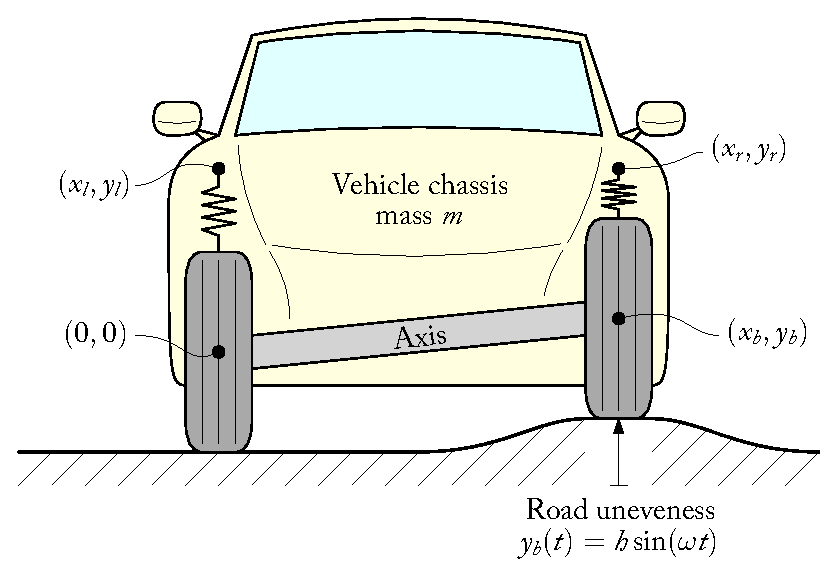
\includegraphics[width=0.7\textwidth]{figures/chapter_4/car_axis}
  \caption{Car-axis dynamics problem~\cite{lioen1998test, mazzia2008test}. The car is modeled as springs connected to two bars. The bottom of the left tire is the origin. The car chassis is represented by a bar of mass $m$. The position of the chassis is given by $\m{q} = [x_l, y_l, x_r, y_r]^\top$. The left tire is always on a flat surface, while the right tire periodically goes over a sinusoidal bump of the form $y_b(t) = h\sin(\omega t)$. The distance between the wheels must always remain fixed, and the car chassis must always have a fixed length.}
  \label{chap4:fig:car_axis}
\end{figure}

The car-axis \ac{DAE} system is solved using the proposed index reduction algorithm. The results are summarized in Table~\ref{chap4:tab:car_axis}. As expected, the index is reduced to 0, and the system is transformed into a set of \acp{ODE}. The complexity of the expressions encountered during the index reduction is given in terms of the number of functions $\cf$, additions $\ca$, multiplications $\cm$, and divisions $\cd$; and, as reported in the table, the index reduction is successful and no expression swell is observed. The reduced system is numerically solved using a and the results are shown in Figure~\ref{chap4:fig:car_axis}, where the springs' lengths are plotted. The left spring is always at its relaxed length, while the right spring periodically changes its length due to the bump. Notably also \Mathematica{} and \Matlab{} (both Pantelides and Gaussian elimination) are able to solve correctly reduce the index of the car-axis problem and integrate the resulting system.

\begin{table}
  \caption{Expression complexity encountered throughout the index reduction of the car-axis problem~\cite{lioen1998test, mazzia2008test} \ac{DAE} system index reduction. \emph{Legend}: $\cf$ = functions, $\ca$ = additions, $\cm$ = multiplications, and $\cd$ = divisions.}
  \label{chap4:tab:car_axis}
  \centering
  {\footnotesize\begin{tabular}{cccc}
    \multicolumn{4}{c}{\textbf{Car-Axis~\cite{lioen1998test, mazzia2008test}}} \\
    \toprule
    \textbf{Original \acp{DAE}} & \multicolumn{3}{c}{$\mF = 108\cf + 131\cm + 56\ca$ \quad $\mh = 0$} \\
    \midrule
    \textbf{Reduction step} & $\mE$ & $\mg$ & $\ma$ \\
    \midrule
    Index-3 \acp{DAE} & $12\cm$ & $94\cf + 145\cm + 54\ca$ & $14\cf + 16\cm + 10\ca$ \\
    Index-2 \acp{DAE} & $12\cm$ & $94\cf + 145\cm + 54\ca$ & $26\cf + 45\cm + 15\ca$ \\
    Index-1 \acp{DAE} & $12\cm$ & $94\cf + 145\cm + 54\ca$ & $136\cf + 4\cd + 261\cm + 95\ca$ \\
    Index-0 \acp{DAE} & $1060\cf + 38\cd + 1901\cm + 717\ca$ & $431\cf + 8\cd + 842\cm + 268\ca$ & $0$ \\
    \midrule
    \textbf{Reduced \acp{DAE}} & \multicolumn{3}{c}{$\mF = 896\cf + 4\cd + 1202\cm + 546\ca$ \quad $\mh = 176\cf + 4\cd + 322\cm + 120\ca$} \\
    \bottomrule
  \end{tabular}}
\end{table}

\begin{figure}[htb]
  \centering
  \small{\includetikz{figures/chapter_4/car_axis_length.tex}}
  \caption{Springs length of the car-axis problem~\cite{lioen1998test, mazzia2008test}. \emph{Legend}: \textcolor{mycolor1}{$\blacksquare$} left spring $L_l = \sqrt{x_l^2 + y_l^2}$, \textcolor{mycolor2}{$\blacksquare$} right spring $L_r = \sqrt{(x_r - x_b)^2 + (y_r - y_b)^2}$.}
  \label{chap4:fig:tppc_initial}
\end{figure}

\subsection{Slider-Crank Mechanism}

The slider-crank mechanism presented in Figure~\ref{chap4:fig:flexible_slider_crank} is a classic problem in mechanical engineering. The mechanism consists of a crank, a connecting rod, and a slider. The crank is driven by a motor, and the slider moves back and forth in a straight line. In this case, the problem is modeled as a flexible \ac{MB} system, hence the rod connecting the crank and the slider is modeled as a flexible beam. The flexible \ac{MBD} problem is posed as a second-order index-3 \acp{DAE} of the form
%
\begin{equation*}
  \begin{cases}
    \m{M}(\m{p}, \m{q})\begin{bmatrix}\m{p}^{\prime\prime} \\ \m{q}^{\prime\prime}\end{bmatrix} - \jac{\bm{\Phi}}{\m{p},\m{q}}(\m{p}, \m{q}, t)^{\top}\bm{\lambda} = \m{f}(\m{p}, \m{p}^{\prime}, \m{q}, \m{q}^{\prime}) \\
    \bm{\Phi}(\m{p}) = \m{0}
  \end{cases} \, \text{,}
  \qquad \text{with} \qquad \jac{\bm{\Phi}}{\m{p},\m{q}}(\m{p}, \m{q}, t) = \dfrac{\partial}{\partial(\m{p}, \m{q})}\bm{\Phi}(\m{p}, \m{q}, t)
  \, \text{,}
\end{equation*}
%
where the position or gross motion coordinates are
%
\begin{equation*}
  \m{p} = \begin{bmatrix}
    \phi_1 \\
    \phi_2 \\
    x_3
  \end{bmatrix} \quad \begin{matrix}
    \text{crank angle,} \\
    \text{connecting rod angle,} \\
    \text{sliding block displacement.}
  \end{matrix}
\end{equation*}
%
The deformation coordinates of the flexible connecting rod are
%
\begin{equation*}
  \m{q} = \begin{bmatrix}
    q_1 \\
    q_2 \\
    q_3 \\
    q_4
  \end{bmatrix} \quad \begin{matrix}
    \text{first lateral mode} \sin(\pi x/\ell_2) \, \text{,} \\
    \text{second lateral mode} \sin(2\pi x/\ell_2) \, \text{,} \\
    \text{longitudinal displacement midpoint,} \\
    \text{longitudinal displacement endpoint.}
  \end{matrix}
\end{equation*}
%
The mass matrix $\m{M}(\m{p}, \m{q})$, and the force vector $\m{f}(\m{p}, \m{q}, \m{p}^\prime, \m{q}^\prime)$ are given by
%
\begin{equation}
  \m{M}(\m{p}, \m{q}) = \begin{bmatrix}
    \m{M}_r(\m{p}) + \m{M}_e(\m{p}, \m{q}) & \m{C}(\m{p}, \m{q})^\top \\
    \m{C}(\m{p}, \m{q})                    & \m{M}_{d}
  \end{bmatrix} \, \text{,}
\end{equation}
%
with rigid motion mass matrix
%
\begin{equation*}
  \m{M}_r(\m{p}) = \begin{bmatrix}
    J_1+m_2 \ell_1^2 & \ell_1 \ell_2 m_2 \cos(\phi_1 - \phi_2)/2 & 0 \\
    \ell_1 \ell_2 m_2 \cos(\phi_1 - \phi_2)/2 & J_2 & 0 \\
    0 & 0 & m_3
  \end{bmatrix} \, \text{,}
\end{equation*}
%
coupling blocks
%
\begin{equation*}
  \m{M}_e(\m{p}, \m{q}) = \small{\begin{bmatrix}
    0 & \rho \ell_1(\cos(\phi_1 - \phi_2)\m{c}_1^\top + \sin(\phi_1 - \phi_2)\m{c}_2^\top) \m{q} & 0 \\
    \rho \ell_1(\cos(\phi_1 - \phi_2)\m{c}_1^\top + \sin(\phi_1 - \phi_2)\m{c}_2^\top) \m{q} & \m{q}^\top\m{M}_{d}\m{q} + 2\rho\m{c}_{12}^\top\m{q} & 0 \\
    0 & 0 & 0
  \end{bmatrix}}
\end{equation*}
%
and
%
\begin{equation*}
  \m{C}(\m{p}, \m{q})^\top = \begin{bmatrix}
    \rho \ell_1(\cos(\phi_1 - \phi_2)\m{c}_2^\top - \sin(\phi_1 - \phi_2)\m{c}_1^\top) \\
    \rho\m{c}_{21}^\top + \rho\m{q}^\top\m{B} \\
    \m{0}^\top
  \end{bmatrix} \, \text{,}
\end{equation*}
%
and elastic body space discretization mass matrix
%
\begin{equation*}
  \m{M}_{d} = \rho d h \ell_2 \begin{bmatrix}
    1/2 & 0   & 0 & 0 \\
    0   & 1/2 & 0 & 0 \\
    0   & 0   & 8 & 1 \\
    0   & 0   & 1 & 2
  \end{bmatrix} \, \text{.}
\end{equation*}
%
The force vector is given by
%
\begin{equation}
  \m{f}(\m{p}, \m{q}, \m{p}^\prime, \m{q}^\prime) = \begin{bmatrix}
    \m{f}_r(\m{p}, \m{p}^\prime) + \m{f}_e(\m{p}, \m{q}, \m{p}^\prime, \m{q}^\prime) \\
    \m{f}_{d}(\m{p}, \m{q}, \m{p}^\prime, \m{q}^\prime) - \mathrm{grad}(\m{W}_{d}(\m{q})) - \m{D}_{d} \m{q}^\prime
  \end{bmatrix} \, \text{.}
\end{equation}
%
where the rigid motion terms are collected in
%
\begin{equation*}
  \m{f}_r(\m{p}, \m{p}^\prime) = \begin{bmatrix}
    -\ell_1(\gamma(m_1 + 2m_2) \cos(\phi_1)/2 + \ell_2 m_2 \phi_2^{\prime2} \sin(\phi_1 - \phi_2)) \\
    -\ell_2 \gamma m_2 \cos(\phi_2)/2 + \ell_1 \ell_2 m_2 \phi_1^{\prime2} \sin(\phi_1 - \phi_2)/2 \\
    0
  \end{bmatrix} \, \text{.}
\end{equation*}
%
For the force term $\m{f}_e(\m{p}, \m{q}, \m{p}^\prime, \m{q}^\prime)$ the expression is
%
\begin{equation*}
  \m{f}_e(\m{p}, \m{q}, \m{p}^\prime, \m{q}^\prime) = \small{\begin{bmatrix}
    \rho \ell_1 \phi_2^{\prime2}(\cos(\phi_1 - \phi_2)\m{c}_2^\top - \sin(\phi_1 - \phi_2)\m{c}_1^\top) \m{q}-2 \rho \ell_1 \phi_2^\prime(\cos(\phi_1 - \phi_2)\m{c}_1^\top + \sin(\phi_1 - \phi_2)\m{c}_2^\top) \m{q}^\prime \\[0.5em]
    \rho \ell_1 \phi_1^{\prime2}(\sin(\phi_1 - \phi_2)\m{c}_1^\top - \cos(\phi_1 - \phi_2)\m{c}_2^\top) \m{q}-2 \rho \phi_2^\prime \m{c}_{12}^\top \m{q}^\prime-2 \phi_2^\prime {\m{q}^\prime}^\top \m{M}_{d} \m{q} \dots\\
    -\rho {\m{q}^\prime}^\top \m{B} \m{q}^\prime - \rho \gamma(\cos(\phi_2) \m{c}_1^\top \m{q} - \sin \phi_2 \m{c}_2^\top \m{q}) \\[0.5em]
    0
\end{bmatrix}} \, \text{,}
\end{equation*}
%
and for $f_{d}(\m{p}, \m{q}, \m{p}^\prime, \m{q}^\prime)$ the expression is
%
\begin{equation*}
  f_{d}(\m{p}, \m{q}, \m{p}^\prime, \m{q}^\prime) = \phi_2^{\prime2} \m{M}_{d} \m{q}+\rho(\phi_2^{\prime2} \m{c}_{12}+\ell_1 \phi_1^{\prime2}(\cos(\phi_1 - \phi_2) \m{c}_1 + \sin(\phi_1 - \phi_2) \m{c}_2)+2 \phi_2^\prime \m{B} \m{q}^\prime)-\rho \gamma\left(\sin \phi_2 \m{c}_1+\cos(\phi_2) \m{c}_2\right) \, \text{.}
\end{equation*}

The gradient of the elastic potential $\m{W}_{d}(\m{q})$ in case of linear elasticity (which is the default) is $\mathrm{grad}(\m{W}_{d}(\m{q})) = \m{K}_{d} \m{q}$ with the stiffness matrix
%
\begin{equation*}
  \m{K}_{d} = \dfrac{E d h}{\ell_2} \begin{bmatrix}
    \pi^4/24(h/\ell_2)^2 & 0                    & 0    & 0    \\
    0                   & \pi^4 2/3(h/\ell_2)^2 & 0    & 0    \\
    0                   & 0                     & 16/3 & -8/3 \\
    0                   & 0                     & -8/3 & 7/3
  \end{bmatrix} \, \text{.}
\end{equation*}
%
Alternatively, in the case of the nonlinear beam model, it holds $\mathrm{grad}(\m{W}_{d}(\m{q})) = K_{d}\m{q} + \m{K}_{d}(\m{q})$, where
%
\begin{equation*}
  \m{K}_{d}(\m{q}) = \dfrac{\pi^2 E d h}{2l_2^2} \begin{bmatrix}
    q_1 q_4 - \beta q_2(-4q_3 + 2q_4) \\
    4 q_2 q_4 - \beta q_1(-4q_3 + 2q_4) \\
    4 \beta q_1 q_2 \\
    q_1^2/2 + 2q_2^2 - 2 \beta q_1 q_2
  \end{bmatrix} \, \text{,}
  %
  \quad \text{with} \quad
  %
  \beta = \dfrac{80}{9\pi^2} \, \text{.}
\end{equation*}
%
The damping matrix $\m{D}_{d}$ is by default zero. The coupling matrices and vectors arising from the space discretization read
%
\begin{equation*}
  \m{B} = d h \ell_2 \begin{bmatrix}
    0             & 0         & -16/\pi^3 & 8/\pi^3-1/\pi \\
    0             & 0         & 0         & 1/(2\pi)      \\
    16/\pi^3      & 0         & 0         & 0             \\
    1/\pi-8/\pi^3 & -1/(2\pi) & 0         & 0
  \end{bmatrix} \, \text{,}
\end{equation*}
%
and
%
\begin{equation*}
  \begin{matrix}
    \m{c}_{1}  = d h \ell_2  \left[ 0,     0,         2/3, 1/6 \right]^\top \, \text{,} \\
    \m{c}_{2}  = d h \ell_2  \left[ 2/\pi, 0,         0,   0   \right]^\top \, \text{,} \\
    \m{c}_{12} = d h \ell_2^2\left[ 0,     0,         1/3, 1/6 \right]^\top \, \text{,} \\
    \m{c}_{21} = d h \ell_2^2\left[ 1/\pi, -1/(2\pi), 0,   0   \right]^\top \, \text{.}
  \end{matrix}
\end{equation*}
%
The constraints of the slider-crank mechanism are given by
%
\begin{equation*}
  \bm{\Phi}(\m{p}) = \begin{bmatrix}
    \ell_1\sin(\phi_1) + \ell_2\sin(\phi_2) + q_4\sin(\phi_2) \\
    x_3 - \ell_1\cos(\phi_1) - \ell_2\cos(\phi_2) - q_4\cos(\phi_2) \\
    \phi_1 - \Omega t \\
  \end{bmatrix} = \m{0} \, \text{.}
\end{equation*}
%
For the simulation, the following parameters are used:
%
\begin{equation*}
  \begin{matrix}
    \ell_1 = \SSI{0.15}{\meter} & \text{body 1 length,} \\
    \ell_2 = \SSI{0.30}{\meter} & \text{body 2 length,} \\
    m_1 = \SSI{0.36}{\kilo\gram} & \text{body 1 mass,} \\
    m_2 = \SSI{0.151104}{\kilo\gram} & \text{body 2 mass,} \\
    m_3 = \SSI{0.075552}{\kilo\gram} & \text{body 3 mass,} \\
    J_1 = \SSI{0.002727}{\kilo\gram\meter\squared} & \text{body 1 moment of inertia,} \\
    J_2 = \SSI{0.0045339259}{\kilo\gram\meter\squared} & \text{body 2 moment of inertia,} \\
    \rho = \SSI{7870}{\kilo\gram\per\meter\cubed} & \text{rod density,} \\
    E = \SSI{200}{\giga\newton\per\meter\squared} & \text{rod Young's modulus,} \\
    \gamma = 0 & \text{gravity constant,} \\
    \Omega = \SSI{150}{\radian\per\second} & \text{prescribed crank angular velocity.} \\
  \end{matrix}
\end{equation*}
%
The initial conditions according to~\cite{lioen1998test, mazzia2008test} are
%
\begin{equation*}
  \m{p}_{0} = \begin{bmatrix}
    0.000000000000000\cdot10^{+0} \\
    0.000000000000000\cdot10^{+0} \\
    4.500169330000000\cdot10^{-1}
  \end{bmatrix} \, \text{,} \qquad
  \m{p}^{\prime}_{0} = \begin{bmatrix}
     1.500000000000000\cdot10^{+2} \\
    -7.499576703969453\cdot10^{+1} \\
    -2.689386719979040\cdot10^{-6}
  \end{bmatrix} \, \text{,}
\end{equation*}
\begin{equation*}
  \m{q}_{0} = \begin{bmatrix}
    0.000000000000000\cdot10^{+0} \\
    0.000000000000000\cdot10^{+0} \\
    1.033398630000000\cdot10^{-5} \\
    1.693279690000000\cdot10^{-5}
  \end{bmatrix} \, \text{,} \qquad
  \m{q}^{\prime}_{0} = \begin{bmatrix}
     4.448961125815990\cdot10^{-1} \\
     4.634339319238670\cdot10^{-3} \\
    -1.785910760000550\cdot10^{-6} \\
    -2.689386719979040\cdot10^{-6}
  \end{bmatrix} \, \text{,}
\end{equation*}
\begin{equation*}
  \bm{\lambda}_{0} = \begin{bmatrix}
     6.552727150584648\cdot10^{-8} \\
    -3.824589509350831\cdot10^{+2} \\
     4.635908708561371\cdot10^{-9}
  \end{bmatrix} \, \text{,}
\end{equation*}
%
and the integration time interval is $t \in \RSI{0}{0.1}{\second}$.

The slider-crank mechanism \ac{DAE} system is solved with the aid of the proposed index reduction algorithm. Specifically, both the linear and nonlinear flexible beam models are considered. The results in terms of expression complexity encountered throughout the index reduction are similar for both formulations, and they are summarized in Table~\ref{chap4:tab:flexible_slider_crank}. As shown in the table, the expression complexity increases significantly during the index reduction process, which is expected due to the complexity of the problem. Hierarchical representation is also employed to limit the expression swelling, and the results are summarized in Table~\ref{chap4:tab:flexible_slider_crank_veil}. The results show that the hierarchical representation reduces the expression complexity by an order of magnitude, which is beneficial for the numerical solution of the \ac{DAE} system. Nevertheless, it must be highlighted that, despite the mitigation of the expression complexity, the hierarchical representation does not prevent the expression complexity from increasing significantly during the index reduction process, which allows us to conclude that this problem is affected by inherent expression swelling. The results of the numerical simulation are shown in Figure~\ref{chap4:fig:flexible_slider_crank}, where the longitudinal displacements $q_3$ and $q_4$ of the flexible beam are illustrated. The results show that the flexible beam undergoes significant and fast deformation during the motion of the slider-crank mechanism, confirming the high stiffness of the \ac{DAE} system. In particular, the nonlinear beam model shows a more pronounced deformation compared to the linear beam model, which makes the numerical solution more challenging.

\begin{figure}[htb]
  \centering
  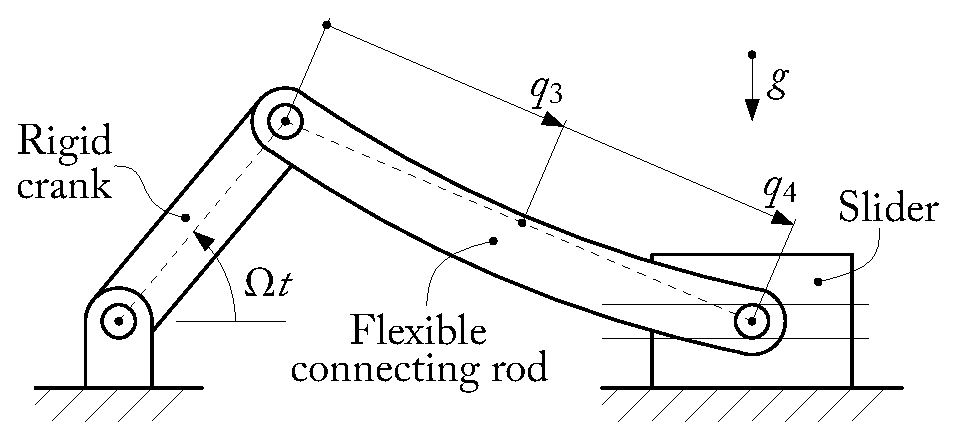
\includegraphics[width=0.475\linewidth]{flexible_slider_crank}
  \caption{Representation of the flexible slider-crank mechanism~\cite{lioen1998test, mazzia2008test}.}
  \label{chap4:fig:flexible_slider_crank}
\end{figure}

\begin{table}
  \caption{Expression complexity encountered throughout the index reduction of the flexible slider-crank mechanism problem~\cite{lioen1998test, mazzia2008test} \ac{DAE} system index reduction. \emph{Legend}: $\cf$ = functions, $\ca$ = additions, $\cm$ = multiplications, and $\cd$ = divisions.}
  \label{chap4:tab:flexible_slider_crank}
  \centering
  \resizebox{\textwidth}{!}{%
  {\footnotesize\begin{tabular}{cccc}
    \multicolumn{4}{c}{\textbf{Flexible Slider-Crank Mechanism~\cite{lioen1998test, mazzia2008test}}} \\
    \toprule
    \textbf{Original \acp{DAE}} & \multicolumn{3}{c}{$\mF = 281\cf + 10\cd + 607\cm + 144\ca$ \quad $\mh = 0$} \\
    \midrule
    \textbf{Reduction step} & $\mE$ & $\mg$ & $\ma$ \\
    \midrule
    Index-3 \acp{DAE} & $64\cf + 9\cd + 1158\cm + 167\ca$ & $395\cf + 15\cd + 5552\cm + 871\ca$ & $12\cf + 5\cm + 6\ca$ \\
    Index-2 \acp{DAE} & $64\cf + 9\cd + 1158\cm + 167\ca$ & $395\cf + 15\cd + 5552\cm + 871\ca$ & $22\cf + 10\cm + 8\ca$ \\
    Index-1 \acp{DAE} & $20\cf + 5\cd + 110\cm + 19\ca$ & $277\cf + 13\cd + 1907\cm + 326\ca$ & $\star (0.4\cf + 2.4\cm + 0.1\ca)\cdot10^{6} + 15\cd$ \\
    Index-0 \acp{DAE} & $\star (0.8\cf + 4.8\cm + 0.3\ca)\cdot10^{5} + 77\cd$ & $\star (5.8\cf + 35.7\cm + 2.2\ca)\cdot10^{6} + 1259\cd$ & $0$ \\
    \midrule
    \textbf{Reduced \acp{DAE}} & \multicolumn{3}{c}{$\star \mF = (5.8\cf + 36.2\cm + 2.2\ca)\cdot10^{6} + 1336\cd$ \quad $\star \mh = (0.5\cf + 2.4\cm + 0.1\ca)\cdot10^{6} + 15\cd$} \\
    \bottomrule
  \end{tabular}}
  }
\end{table}

\begin{table}
  \caption{Expression complexity encountered throughout the index reduction with the aid of hierarchical representation of the flexible slider-crank mechanism problem~\cite{lioen1998test, mazzia2008test} \ac{DAE} system index reduction. \emph{Legend}: $\cf$ = functions, $\cv$ = veiling variables, $\ca$ = additions, $\cm$ = multiplications, and $\cd$ = divisions.}
  \label{chap4:tab:flexible_slider_crank_veil}
  \centering
  \resizebox{\textwidth}{!}{%
  {\footnotesize\begin{tabular}{cccc}
    \multicolumn{4}{c}{\textbf{Flexible Slider-Crank Mechanism~\cite{lioen1998test, mazzia2008test}}} \\
    \toprule
    \textbf{Original \acp{DAE}} & \multicolumn{3}{c}{$\mF = 281\cf + 10\cd + 607\cm + 144\ca$ \quad $\mh = 0$} \\
    \midrule
    \textbf{Reduction step} & $\mE$ & $\mg$ & $\ma$ \\
    \midrule
    Index-3 \acp{DAE} & $28\cf + 1\cv + 7\cd + 160\cm + 28\ca$ & $91\cf + 2\cv + 8\cd + 291\cm + 44\ca$ & $12\cf + 5\cm + 6\ca$ \\
    Index-2 \acp{DAE} & $18\cf + 1\cv + 6\cd + 88\cm + 15\ca$ & $101\cf + 5\cv + 10\cd + 360\cm + 58\ca$ & $22\cf + 10\cm + 8\ca$ \\
    Index-1 \acp{DAE} & $10\cf + 1\cv + 4\cd + 39\cm + 6\ca$ & $93\cf + 4\cv + 9\cd + 294\cm + 48\ca$ & $10\cf + 2\cv + 9\cd + 82\cm + 14\ca$ \\
    Index-0 \acp{DAE} & $(0.2\cf  + 1.1\cm + 0.1\ca)\cdot10^{6} + 1171\cv + 1158\cd$ & $(0.7\cf + 3.6\cm + 0.4\ca)\cdot10^{5} + 137\cv + 1172\cd$ & $0$ \\
    \midrule
    \textbf{Reduced \acp{DAE}} & \multicolumn{3}{c}{$\mF = (0.3\cf + 1.5\cm + 0.1\ca)\cdot10^{6} + 1308\cv + 2330\cd$ \quad $\mh = 44\cf + 6\cv + 2\cd + 97\cm + 28\ca$} \\
    \bottomrule \\[0.5em]
  \end{tabular}
  }}
  {\footnotesize\begin{tabular}{cc}
    \multicolumn{2}{c}{Hierarchical representation details (9 veils)} \\
    \toprule
    \textbf{Original \acp{DAE}} & $\mv = 0$ \\
    \midrule
    \textbf{Reduction step} & $\mv$ \\
    \midrule
    Index-3 \acp{DAE} & $309\cf + 1\cv + 7\cd + 2946\cm + 485\ca$ \\
    Index-2 \acp{DAE} & $309\cf + 1\cv + 7\cd + 2946\cm + 485\ca$ \\
    Index-1 \acp{DAE} & $422\cf + 7\cv + 14\cd + 3249\cm + 541\ca$ \\
    Index-0 \acp{DAE} & $492919\cf + 63922\cv + 138\cd + 2441245\cm + 155539\ca$ \\
    \midrule
    \textbf{Reduced \acp{DAE}} & $\mv = 492919\cf + 63922\cv + 138\cd + 2441245\cm + 155539\ca$ \\
    \bottomrule
  \end{tabular}}
\end{table}

\begin{figure}[htb]
  \centering
  \small{\includetikz{figures/chapter_4/flexible_slider_crank.tex}}
  \caption{Longitudinal displacement endpoint of the in the flexible slider-crank problem~\cite{lioen1998test, mazzia2008test}. \emph{Color legend}: \textcolor{mycolor2}{$\blacksquare$} longitudinal displacement $q_3$ at the rod midpoint, and \textcolor{mycolor1}{$\blacksquare$} longitudinal displacement $q_4$ at the rod endpoint. \emph{Line legend}: \textbf{---} linear beam model, and \textbf{--~--} nonlinear beam model.}
  \label{chap4:fig:flexible_slider_crank}
\end{figure}

\subsection{The Multi-Pendula System}

The multi-pendula system consists of a chain of $p$ coupled pendula. The first pendulum is an ordinary pendulum, while the remaining pendula are coupled to the previous one. Specifically, the tension in pendulum $i - 1$, which is represented by the Lagrange multiplier $\lambda_{i-1}$, has a small effect on the length of
pendulum $p$, for $i = 2, \dots, p$. The first-order equations of motion for the multi-pendula system are the following~\cite{nedialkov2008solvingIII}
%
\begin{equation}
  \begin{cases}
    u_1^{\prime} = x_1 \\
    v_1^{\prime} = y_1 \\
    x_1^{\prime} = -\lambda_1 x_1 \\
    y_1^{\prime} = -\lambda_1 y_1 - g \\
    x_1^2 + y_1^2 = \ell^2 \\
  \end{cases}
  \quad \text{and} \qquad
  \begin{cases}
    u_i^{\prime} = x_i \\
    v_i^{\prime} = y_i \\
    x_i^{\prime} = -\lambda_p x_i \\
    y_i^{\prime} = -\lambda_p y_i - g \\
    x_i^2 + y_i^2 = (\ell + c\lambda_{i-1})^2
  \end{cases}
  \quad \text{for} \quad i = 2, \dots, p \, \text{.}
  \label{chap4:eq:multi_pendula}
\end{equation}
%
where $x_i, y_i$ and $u_i, v_i$ are the generalized coordinates and velocities of $i$-th pendulum mass. The parameters of the multi-pendula system are chosen as $\ell = \SI{1}{\meter}$, $g = \SI{9.81}{\meter\per\second\squared}$, and $c = 0.1$. The system~\eqref{chap4:eq:multi_pendula} leads to a class of \acp{DAE} of arbitrary size $5p$ and index $2p+1$~\cite{nedialkov2008solvingIII}. Initial conditions are chosen randomly, and the time interval is $t \in \RSI{0}{60}{\second}$.

Here, we consider up to $p = 4$ pendula, leading to a \ac{DAE} system of $20$ variables and index $9$. The computational complexities encountered during the index reduction process are summarized in Table~\ref{chap4:tab:pendula_2}, for the 2-pendula problem, Table~\ref{chap4:tab:pendula_3}, for the 3-pendula problem, Table~\ref{chap4:tab:pendula_4}, for the 4-pendula problem, and lastly Table~\ref{chap4:tab:pendula_5}, for the 5-pendula problem. Multi-pendula systems with $p \leq 3$ exhibit low computational complexity growth during the index reduction process. However, for $p \geq 4$, there is a substantial expression swell, which makes the index reduction process time-consuming and computationally demanding.
%The introduction of veiling variables proved to be effective in reducing the expression complexity, as shown in Tables~\ref{chap4:tab:pendula_4_veil} and \ref{chap4:tab:pendula_5_veil}.
The introduction of veiling variables is avoided on purpose to assess the impact of the expression swelling on the stability of the numerical solution.
It is worth noting that with $p = 4$ the maximum computational complexity that \Maple{} can handle within a reasonable time is reached. For this reason, performing the last reduction steps for $p = 4$ requires a significant amount of time and computational resources. Moreover, we believe that reducing the index of the \ac{DAE} system for $p > 5$ is not feasible with the current computational resources, even with the aid of hierarchical representation. The numerical integration results of the 5-pendula system are depicted in Figure~\ref{chap4:fig:npendula_length}, where the pendula lengths are illustrated in the time interval $t \in \RSI{0}{60}{\second}$.

\begin{table}
  \caption{Expression complexity encountered throughout the index reduction of the 2-pendula problem~\cite{nedialkov2008solvingIII} \ac{DAE} system index reduction. \emph{Legend}: $\cf$ = functions, $\ca$ = additions, $\cm$ = multiplications, and $\cd$ = divisions.}
  \label{chap4:tab:pendula_2}
  \centering
  {\footnotesize\begin{tabular}{cccc}
    \multicolumn{4}{c}{\textbf{2-Pendula~\cite{pryce1998solving}}} \\
    \toprule
    \textbf{Original \acp{DAE}} & \multicolumn{3}{c}{$\mF = 33\cf + 15\cm + 15\ca$ \quad $\mh = 0$} \\
    \midrule
    \textbf{Reduction step} & $\mE$ & $\mg$ & $\ma$ \\
    \midrule
    Index-5 \acp{DAE} & $0$                  & $12\cf + 8\cm + 2\ca$ & $6\cf + 12\cm + 6\ca$ \\
    Index-4 \acp{DAE} & $1\cf + 5\cm + 1\ca$ & $16\cf + 12\cm + 3\ca$ & $4\cf + 4\cm + 1\ca$ \\
    Index-3 \acp{DAE} & $1\cf + 5\cm + 1\ca$ & $16\cf + 12\cm + 3\ca$ & $7\cf + 12\cm + 4\ca$ \\
    Index-2 \acp{DAE} & $1\cf + 5\cm + 1\ca$ & $16\cf + 12\cm + 3\ca$ & $18\cf + 2\cd + 30\cm + 9\ca$ \\
    Index-1 \acp{DAE} & $1\cf + 5\cm + 1\ca$ & $16\cf + 12\cm + 3\ca$ & $118\cf + 2\cd + 283\cm + 72\ca$ \\
    Index-0 \acp{DAE} & $555\cf + 21\cd + 1213\cm + 287\ca$ & $16\cf + 12\cm + 3\ca$ & $0$ \\
    \midrule
    \textbf{Reduced \acp{DAE}} & \multicolumn{3}{c}{
    $\mF = 482\cf + 2\cd + 807\cm + 229\ca$ \quad $\mh = 153\cf + 4\cd + 341\cm + 92\ca$} \\
    \bottomrule
  \end{tabular}}
\end{table}

\begin{table}
  \caption{Expression complexity encountered throughout the index reduction of the 3-pendula problem~\cite{nedialkov2008solvingIII} \ac{DAE} system index reduction. \emph{Legend}: $\cf$ = functions, $\ca$ = additions, $\cm$ = multiplications, and $\cd$ = divisions.}
  \label{chap4:tab:pendula_3}
  \centering
  {\footnotesize\begin{tabular}{cccc}
    \multicolumn{4}{c}{\textbf{3-Pendula~\cite{nedialkov2008solvingIII}}} \\
    \toprule
    \textbf{Original \acp{DAE}} & \multicolumn{3}{c}{$\mF = 50\cf + 23\cm + 23\ca$ \quad $\mh = 0$} \\
    \midrule
    \textbf{Reduction step} & $\mE$ & $\mg$ & $\ma$ \\
    \midrule
    Index-7 \acp{DAE} & $0$                   & $18\cf + 12\cm + 3\ca$ & $10\cf + 21\cm + 10\ca$ \\
    Index-6 \acp{DAE} & $2\cf + 10\cm + 2\ca$ & $26\cf + 20\cm + 5\ca$ & $4\cf + 4\cm + 1\ca$ \\
    Index-5 \acp{DAE} & $2\cf + 10\cm + 2\ca$ & $26\cf + 20\cm + 5\ca$ & $7\cf + 12\cm + 4\ca$ \\
    Index-4 \acp{DAE} & $2\cf + 10\cm + 2\ca$ & $26\cf + 20\cm + 5\ca$ & $18\cf + 2\cd + 30\cm + 9\ca$ \\
    Index-3 \acp{DAE} & $2\cf + 10\cm + 2\ca$ & $26\cf + 20\cm + 5\ca$ & $118\cf + 2\cd + 283\cm + 72\ca$ \\
    Index-2 \acp{DAE} & $2\cf + 10\cm + 2\ca$ & $26\cf + 20\cm + 5\ca$ & $992\cf + 3\cd + 2077\cm + 479\ca$ \\
    Index-1 \acp{DAE} & $2\cf + 10\cm + 2\ca$ & $26\cf + 20\cm + 5\ca$ & $6824\cf + 3\cd + 17665\cm + 4030\ca$ \\
    Index-0 \acp{DAE} & $54152\cf + 51\cd + 136388\cm + 28945\ca$ & $26\cf + 20\cm + 5\ca$ & $0$ \\
    \midrule
    \textbf{Reduced \acp{DAE}} & \multicolumn{3}{c}{
    $\mF = 28319\cf + 3\cd + 64295\cm + 15806\ca$ \quad $\mh = 7973\cf + 10\cd + 20092\cm + 4605\ca$} \\
    \bottomrule
  \end{tabular}}
\end{table}

\begin{table}
  \caption{Expression complexity encountered throughout the index reduction of the 4-pendula problem~\cite{nedialkov2008solvingIII} \ac{DAE} system index reduction. \emph{Legend}: $\cf$ = functions, $\ca$ = additions, $\cm$ = multiplications, and $\cd$ = divisions.}
  \label{chap4:tab:pendula_4}
  \centering
  {\footnotesize\begin{tabular}{cccc}
    \multicolumn{4}{c}{\textbf{4-Pendula~\cite{nedialkov2008solvingIII}}} \\
    \toprule
    \textbf{Original \acp{DAE}} & \multicolumn{3}{c}{$\mF = 67\cf + 31\cm + 31\ca$ \quad $\mh = 0$} \\
    \midrule
    \textbf{Reduction step} & $\mE$ & $\mg$ & $\ma$ \\
    \midrule
    Index-9 \acp{DAE} & $0$                   & $24\cf + 16\cm + 4\ca$ & $14\cf + 30\cm + 14\ca$ \\
    Index-8 \acp{DAE} & $3\cf + 15\cm + 3\ca$ & $36\cf + 28\cm + 7\ca$ & $4\cf + 4\cm + 1\ca$ \\
    Index-7 \acp{DAE} & $3\cf + 15\cm + 3\ca$ & $36\cf + 28\cm + 7\ca$ & $7\cf + 12\cm + 4\ca$ \\
    Index-6 \acp{DAE} & $3\cf + 15\cm + 3\ca$ & $36\cf + 28\cm + 7\ca$ & $18\cf + 2\cd + 30\cm + 9\ca$ \\
    Index-5 \acp{DAE} & $3\cf + 15\cm + 3\ca$ & $36\cf + 28\cm + 7\ca$ & $118\cf + 2\cd + 283\cm + 72\ca$ \\
    Index-4 \acp{DAE} & $3\cf + 15\cm + 3\ca$ & $36\cf + 28\cm + 7\ca$ & $992\cf + 3\cd + 2077\cm + 479\ca$ \\
    Index-3 \acp{DAE} & $3\cf + 15\cm + 3\ca$ & $36\cf + 28\cm + 7\ca$ & $6824\cf + 3\cd + 17665\cm + 4030\ca$ \\
    Index-2 \acp{DAE} & $3\cf + 15\cm + 3\ca$ & $36\cf + 28\cm + 7\ca$ & $(4.8\cf + 4\cd + 11.9\cm + 2.7\ca)\cdot10^{5}$ \\
    Index-1 \acp{DAE} & $3\cf + 15\cm + 3\ca$ & $36\cf + 28\cm + 7\ca$ & $\star (3.0\cf + 14.9\cm + 0.4\ca)\cdot10^{6} + 4\cd$ \\
    Index-0 \acp{DAE} & $\star (3.0\cf + 14.7\cm + 0.4\ca)\cdot10^{7} + 92\cd$ & $30\cf + 28\cm + 7\ca$ & $0$ \\
    \midrule
    \textbf{Reduced \acp{DAE}} & \multicolumn{3}{c}{
    $\star \mF = (3.0\cf + 14.7\cm + 0.4\ca)\cdot10^{7} + 92\cd$ \quad $\star \mh = (3.1\cf + 15.1\cm + 0.5\ca)\cdot10^{6} + 18\cd$} \\
    \bottomrule
  \end{tabular}}
\end{table}

\begin{table}
  \caption{Expression complexity encountered throughout the index reduction of the 5-pendula problem~\cite{nedialkov2008solvingIII} \ac{DAE} system index reduction. \emph{Legend}: $\cf$ = functions, $\ca$ = additions, $\cm$ = multiplications, and $\cd$ = divisions.}
  \label{chap4:tab:pendula_5}
  \centering
  {\footnotesize\begin{tabular}{cccc}
    \multicolumn{4}{c}{\textbf{5-Pendula~\cite{nedialkov2008solvingIII}}} \\
    \toprule
    \textbf{Original \acp{DAE}} & \multicolumn{3}{c}{$\mF = 84\cf + 39\cm + 39\ca$ \quad $\mh = 0$} \\
    \midrule
    \textbf{Reduction step} & $\mE$ & $\mg$ & $\ma$ \\
    \midrule
    Index-11 \acp{DAE} & $0$                   & $30\cf + 20\cm + 5\ca$ & $18\cf + 39\cm + 18\ca$ \\
    Index-10 \acp{DAE} & $4\cf + 20\cm + 4\ca$ & $46\cf + 36\cm + 9\ca$ & $4\cf + 4\cm + 1\ca$ \\
    Index-9 \acp{DAE}  & $4\cf + 20\cm + 4\ca$ & $46\cf + 36\cm + 9\ca$ & $7\cf + 12\cm + 4\ca$ \\
    Index-8 \acp{DAE}  & $4\cf + 20\cm + 4\ca$ & $46\cf + 36\cm + 9\ca$ & $18\cf + 2\cd + 30\cm + 9\ca$ \\
    Index-7 \acp{DAE}  & $4\cf + 20\cm + 4\ca$ & $46\cf + 36\cm + 9\ca$ & $118\cf + 2\cd + 283\cm + 72\ca$ \\
    Index-6 \acp{DAE}  & $4\cf + 20\cm + 4\ca$ & $46\cf + 36\cm + 9\ca$ & $992\cf + 3\cd + 2077\cm + 479\ca$ \\
    Index-5 \acp{DAE}  & $4\cf + 20\cm + 4\ca$ & $46\cf + 36\cm + 9\ca$ & $6824\cf + 3\cd + 17665\cm + 4030\ca$ \\
    Index-4 \acp{DAE}  & $4\cf + 20\cm + 4\ca$ & $46\cf + 36\cm + 9\ca$ & $(4.8\cf + 4\cd + 11.9\cm + 2.7\ca)\cdot10^{5}$ \\
    Index-3 \acp{DAE}  & $4\cf + 20\cm + 4\ca$ & $46\cf + 36\cm + 9\ca$ & $\star (3.0\cf + 14.9\cm + 0.4\ca)\cdot10^{6} + 4\cd$ \\
    Index-2 \acp{DAE}  & $4\cf + 20\cm + 4\ca$ & $46\cf + 36\cm + 9\ca$ & $\star (5.1\cf + 4.0\cm + 1.3\ca)\cdot10^{7} + 5\cd$ \\
    Index-1 \acp{DAE}  & $4\cf + 20\cm + 4\ca$ & $46\cf + 36\cm + 9\ca$ & $\star (9.1\cf + 11.3\cm + 5.9\ca)\cdot10^{7} + 5\cd$ \\
    Index-0 \acp{DAE}  & $\star (8.8\cf + 7.2\cm + 1.0\ca)\cdot10^{8} + 5\cd$ & $46\cf + 36\cm + 9\ca$ & $0$ \\
    \midrule
    \textbf{Reduced \acp{DAE}} & \multicolumn{3}{c}{
    $\star \mF = \star (8.8\cf + 7.2\cm + 1.0\ca)\cdot10^{8} + 5\cd$ \quad $\star \mh = (9.2\cf + 6.5\cm + 1.0\ca)\cdot10^{7} + 18\cd$} \\
    \bottomrule
  \end{tabular}}
\end{table}

\begin{figure}[htb]
  \centering
  \small{\includetikz{figures/chapter_4/npendula_length.tex}}
  \caption{Pendula lengths of the multi-pendula problem~\cite{nedialkov2008solvingIII} (up to 5 pendula). \emph{Legend}: \textcolor{mycolor1}{$\blacksquare$} 1\textsuperscript{st} pendulum length $\ell_1 = \ell$, \textcolor{mycolor2}{$\blacksquare$} 2\textsuperscript{nd} pendulum length $\ell_2 = \ell + c\lambda_1$, \textcolor{mycolor3}{$\blacksquare$} 3\textsuperscript{rd} pendulum length $\ell_3 = \ell + c\lambda_2$, \textcolor{mycolor4}{$\blacksquare$} 4\textsuperscript{th} pendulum length $\ell_4 = \ell + c\lambda_3$, and \textcolor{mycolor5}{$\blacksquare$} 5\textsuperscript{th} pendulum length $\ell_5 = \ell + c\lambda_4$.}
  \label{chap4:fig:npendula_length}
\end{figure}

\subsection{Double-Wishbone Suspension System}

As a final example for this application field, a consider double-wishbone suspension system.

\subsubsection{Suspension System Modeling}

Double A-arm or double wishbone suspensions are independent suspension systems widely used in the automotive industry, especially in high-performance vehicles, due to their superior handling characteristics. The studied double A-arm suspension system, shown in Figure~\ref{chap4:fig:suspension_render} is characterized by two A-shaped arms, one upper and one lower, connected to the chassis at one end and to the wheel carrier at the other end forming, together with the tie rod, the principal kinematic chain of the suspension system. A second kinematic chain is formed by the push rod and the rocker, which transfer the vertical load from the wheel carrier to the shock absorber.

\begin{figure}[htb]
  \begin{minipage}[c]{0.485\linewidth}
    \centering
    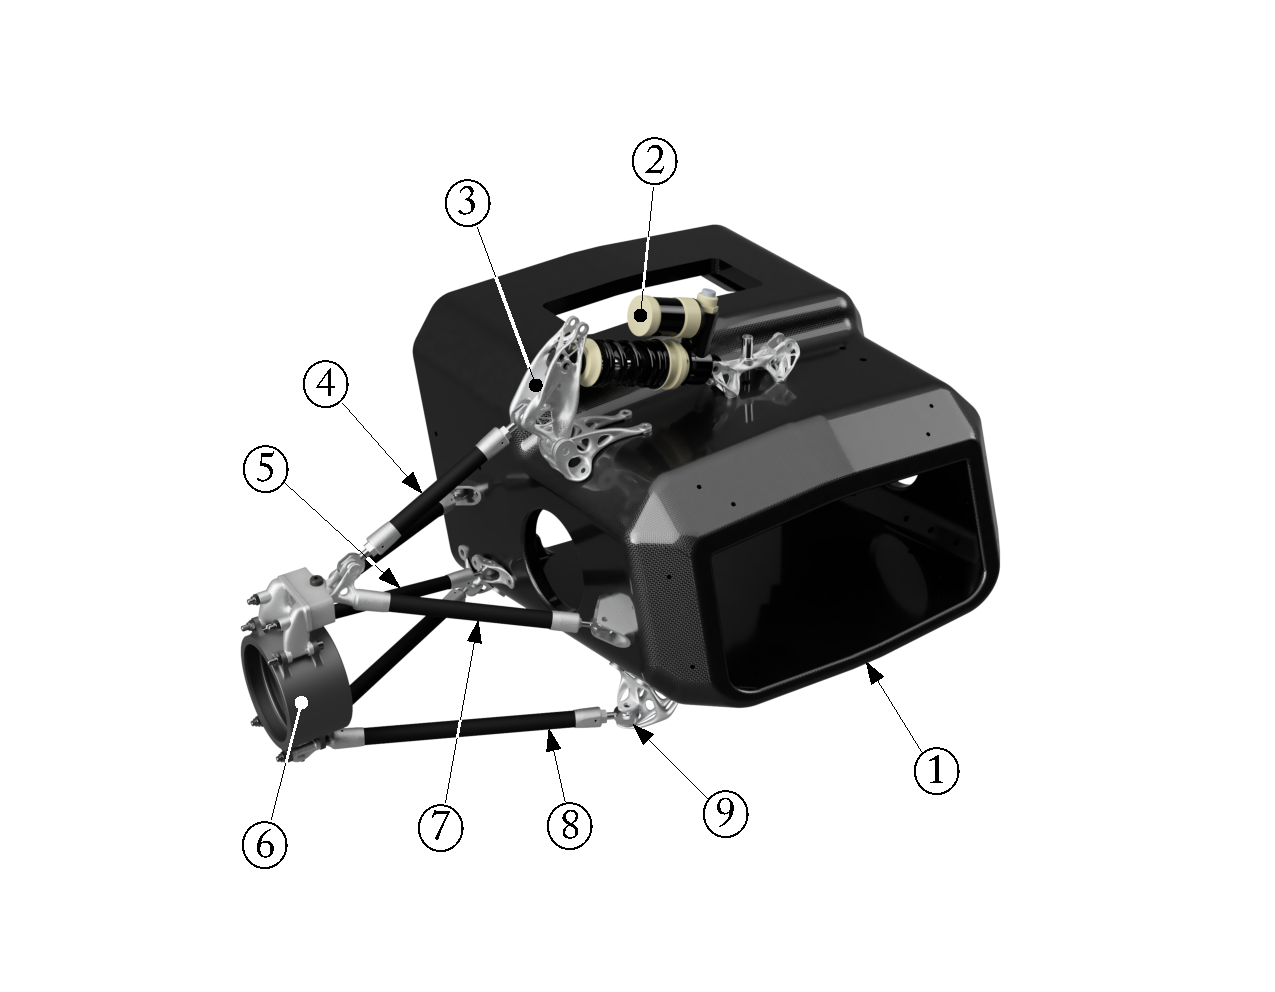
\includegraphics[width=1.0\textwidth, trim={3.0cm 1.5cm 4.0cm 1.7cm}, clip]{figures/chapter_4/suspension_render.eps}
  \end{minipage}
  %\hfill
  \begin{minipage}[c]{0.45\linewidth}
    \centering
    \small{\begin{tabular}{ccc}
      \toprule
      \multirow{2}{*}{\textbf{\#}} & \multirow{2}{*}{\textbf{Component}} & \textbf{\TrussMe{}} \\
      & & \textbf{type} \\
      \midrule
      \circled{\small{1}} & Carbon fiber cell & Rigid support    \\[1.25mm]
      \circled{\small{2}} & Shock absorber    & Constrained node \\[1.25mm]
      \circled{\small{3}} & Rocker            & Generic element  \\[1.25mm]
      \circled{\small{4}} & Push rod          & Rod element      \\[1.25mm]
      \circled{\small{5}} & Tie rod           & Rod element      \\[1.25mm]
      \circled{\small{6}} & Wheel carrier     & Generic element  \\[1.25mm]
      \circled{\small{7}} & Upper wishbone    & Beam elements    \\[1.25mm]
      \circled{\small{8}} & Lower wishbone    & Beam elements    \\[1.25mm]
      \circled{\small{9}} & Rod end           & Compliant node    \\
      \bottomrule
    \end{tabular}}
  \end{minipage}
  \caption{Rendering and description of the \TrussMe{} elements \citep{trussme} used to model the rear left double wishbone suspension of the Formula SAE \textit{E-Agle Trento Racing Team} vehicle~\citep{eagle}.}
  \label{chap4:fig:suspension_render}
\end{figure}

In this example, the double A-arm suspension compliance is modeled using macro elements, which are modeled through the \TrussMe{} package~\cite{trussme}, which is a \Maple{} package for the symbolic modeling of compliant structures. Details on the modeling of the compliant elements are reported in Appendix~\ref{app4:trussme}. With the approach there presented, two suspension compliance models are generated one does not include the bushings compliance, while the other does. The linear systems have different sizes depending on the number of \acp{DOF} considered. In the case of the suspension without bushings, the system is composed of 78 \acp{DOF}, and has the following form
%
\begin{equation}
  \begin{bmatrix}
    \m{K}_{ff ,\, 42 \times 42}(\mathbb{R}) & \m{K}_{fs ,\, 42 \times 36}(\mathbb{R}) \\
    \m{K}_{sf ,\, 36 \times 42}(\mathbb{R}) & \m{K}_{ss ,\, 36 \times 36}(\mathbb{R})
  \end{bmatrix} \begin{bmatrix}
    \m{d}_{f ,\, 42 \times 1}(\mathbb{R}) \\ \m{d}_{s ,\, 36 \times 1}(\mathbb{R})
  \end{bmatrix} = \begin{bmatrix}
    \m{f}_{f ,\, 42 \times 1}(\mathbb{R}) \\ \m{f}_{s ,\, 36 \times 1}(\mathbb{R})
  \end{bmatrix}
  \, \text{.}
\end{equation}
%
On the other hand, the suspension model with the bushings influence is composed of 138 \acp{DOF}
%
\begin{equation}
  \begin{bmatrix}
    \m{K}_{ff ,\, 72 \times 72}(\mathbb{R}) & \m{K}_{fs ,\, 72 \times 66}(\mathbb{R}) \\
    \m{K}_{sf ,\, 66 \times 72}(\mathbb{R}) & \m{K}_{ss ,\, 66 \times 66}(\mathbb{R})
  \end{bmatrix} \begin{bmatrix}
    \m{d}_{f ,\, 72 \times 1}(\mathbb{R}) \\ \m{d}_{s ,\, 66 \times 1}(\mathbb{R})
  \end{bmatrix} = \begin{bmatrix}
    \m{f}_{f ,\, 72 \times 1}(\mathbb{R}) \\ \m{f}_{s ,\, 66 \times 1}(\mathbb{R})
  \end{bmatrix}
  \, \text{,}
\end{equation}
%
where the additional 60 \acp{DOF} are related to the compliance of the bushings. Both systems are solved using the technique presented in Appendix~\ref{app4:trussme} the, given the generic compliant mechanism described by the linear system of equations
%
\begin{equation}
  \label{chap4:eq:macrofe}
  \underbrace{\begin{bmatrix}
    \m{K}_{ff} & \m{K}_{fs} \\
    \m{K}_{sf} & \m{K}_{ss}
  \end{bmatrix}}_{\textstyle\m{K}} \underbrace{\begin{bmatrix}
    \m{d}_{f} \\ \m{d}_{s}
  \end{bmatrix}}_{\textstyle\m{d}} = \underbrace{\begin{bmatrix}
    \m{f}_{f} \\ \m{f}_{s}
  \end{bmatrix}}_{\textstyle\m{f}} \, \text{,}
  %
  \qquad \text{is sequentially solved as} \qquad
  %
  \begin{aligned}
    \m{d}_{f} &= \m{K}_{ff}^{-1}\left(\m{f}_{f} - \m{K}_{fs}\m{d}_{s}\right) \, \text{,} \\
    \m{f}_{s} &= \m{K}_{sf}\m{d}_{f} + \m{K}_{ss}\m{d}_{s} \, \text{,}
  \end{aligned}
\end{equation}
%
where subscripts $s$ and $f$ indicate respectively the specified and the free \acp{DOF}. Notice that the free and the specified \acp{DOF} are those that are and are not constrained by the boundary conditions, respectively.

The dynamic characteristic of the system is modeled through a \ac{DAE} system of the following type:
%
\begin{subequations}
  \label{chap4:eq:daes}
  \begin{empheq}[left = {\empheqlbrace}, right = {\, \text{,}}]{align}
    & \m{y} = \m{q} + \m{d} \label{chap4:eq:sy} \\
    & \m{M}(\m{y}) \ddot{\m{y}} + \m{r}(\m{q}, \dot{\m{q}}, \m{d}, \dot{\m{d}}) = \m{f}(t) \label{chap4:eq:cr} \\
    & \boldsymbol{\Phi}_{\m{q}}(\m{q})^\top \boldsymbol{\lambda} = \m{r}(\m{q}, \dot{\m{q}}, \m{d}, \dot{\m{d}}) + \m{b}(\m{q}, \dot{\m{q}}, t) \label{chap4:eq:em} \\
    & \boldsymbol{\Phi}(\m{q}) = \m{0} \label{chap4:eq:bc}
  \end{empheq} \\[-2.5em]
  \begin{equation}
    \label{chap4:eq:emf}
    \text{with} \quad \m{r}(\m{q}, \dot{\m{q}}, \m{d}, \dot{\m{d}}) = \m{K}_c(\m{q}) \m{d} + \m{C}_c(\m{q}) \dot{\m{d}} \text{,}
  \end{equation}
\end{subequations}
%
where $\m{q}$ is the state vector, and $t$ is the time. The quantity $\m{d}$ represents the compliance contribution of the mechanism members' deformation. States and deformations are conveniently condensed in a single variable $\m{y}$ as in~\eqref{chap4:eq:sy}. Equation~\eqref{chap4:eq:cr} represents the compliance contribution to the dynamics of the system, where $\m{K}_c$, and $\m{C}_c$ are the stiffness and damping matrices of the compliant bodies, respectively. The matrix $\m{M}$ represents the mass of the mechanism, while $\m{f}$ is the vector of external forces. For convenience, we collect $\m{r}$ in Equation~\eqref{chap4:eq:emf} as the vector of internal forces at the compliant joint. Notice that the product $\m{K}_c(\m{q}) \m{d}$ can be computed through the symbolic solution of the linear systems~\eqref{chap4:eq:macrofe}. Equation~\eqref{chap4:eq:em} represents the equilibrium equations between the rigid and compliant parts of the suspension. Specifically, $\boldsymbol{\Phi}_{\m{q}}$ is the Jacobian matrix of the constraint vector $\boldsymbol{\Phi}$ with respect to the coordinates $\m{q}$, while $\m{b}$ is the vector of external forces applied to the rigid part of the suspension. Lastly, Equation~\eqref{chap4:eq:bc} represents the kinematic constraints of the system. The pick-up points of the modeled suspension are reported in Table~\ref{chap4:tab:positions}. It is possible to derive the lengths of the various elements from these coordinates and to impose constraints to ensure a proper assembling of the mechanism. Components and materials specifications are reported in Tables~\ref{chap4:tab:components} and~\ref{chap4:tab:materials}, respectively.

To consider the compliance contribution as a superposed effect we first assume that the influence of the members' deformation $\m{d}$ is small with respect to the dimensions of the mechanism itself, and thus to the state vector $\m{q}$, \ie{}, $\m{d} \ll \m{q}$. From~\eqref{chap4:eq:sy} it follows that $\m{M}(\m{y}) \approx \m{M}(\m{q})$. It is then possible to split the resolution of the \acp{DAE}~\eqref{chap4:eq:daes} into two stages. Firstly, the implicit differential equation~\eqref{chap4:eq:em} and the manifold~\eqref{chap4:eq:bc} are integrated. Nonetheless, these equations are of an index-3 \ac{MB} \acp{DAE} system of the type~\eqref{chap4:eq:mbd_fo}, which can be reduced to an index-0 or index-1 \acp{DAE} system and solved as above explained. Then, the second stage consists of adding the stationary contribution of the members' deformation $\m{d}$ to the state vector $\m{q}$, that is $\m{y} = \m{q} + \m{d} = \m{q} + \m{K}_c(\m{q})^{-1} (\m{f}(t) - \m{M}(\m{q})\ddot{\m{q}})$.

\begin{table}[htb]
  \caption[Table]{Suspension pick-up points' coordinates in the nominal position.}
  \label{chap4:tab:positions}
  \centering
  \small{\begin{tabular}{cccccc}
    \toprule
    \multirow{2.5}{*}{\shortstack{\textbf{Pick-up} \\ \textbf{point name}}} &
    \multicolumn{2}{c}{\multirow{2.5}{*}{\textbf{Constrained elements}}} &
    \multicolumn{3}{c}{\textbf{Coordinates}} \\ \cmidrule(r{4pt}l{4pt}){4-6}
    & & & $x$\,(\si{\milli\meter}) & $y$\,(\si{\milli\meter}) & $z$\,(\si{\milli\meter}) \\
    \midrule
    $P_{1}$  & Chassis       & Upper-front rod & $-719$  & $270$ & $240$ \\ %(3)
    $P_{2}$  & Chassis       & Upper-rear rod  & $-1010$ & $265$ & $225$ \\ %(4)
    $P_{3}$  & Chassis       & Lower-front rod & $-730$  & $265$ & $120$ \\ %(1)
    $P_{4}$  & Chassis       & Lower-rear rod  & $-1010$ & $235$ &  $98$ \\ %(2)
    $P_{5}$  & Chassis       & Tie rod         & $-775$  & $265$ & $163$ \\ %(5)
    $P_{6}$  & Chassis       & Rocker          & $-895$  & $243$ & $375$ \\ %(13)
    $P_{7}$  & Chassis       & Shock absorber  & $-895$  &  $50$ & $412$ \\ %(15)
    $P_{8}$  & Wheel carrier & Upper-front rod & $-895$  & $517$ & $293$ \\ %(6)
    $P_{9}$  & Wheel carrier & Upper-rear rod  & $-895$  & $517$ & $293$ \\ %(6)
    $P_{10}$ & Wheel carrier & Lower-front rod & $-885$  & $550$ & $120$ \\ %(7)
    $P_{11}$ & Wheel carrier & Lower-rear rod  & $-885$  & $550$ & $120$ \\ %(7)
    $P_{12}$ & Wheel carrier & Tie rod         & $-790$  & $532$ & $198$ \\ %(8)
    $P_{13}$ & Rocker        & Shock absorber  & $-895$  & $236$ & $466$ \\ %(14)
    $P_{14}$ & Rocker        & Push rod        & $-895$  & $280$ & $418$ \\ %(12)
    $P_{15}$ & Push rod      & Wheel carrier   & $-895$  & $479$ & $312$ \\ %(11)
    \bottomrule
  \end{tabular}}
\end{table}

\noindent
\begin{minipage}[c]{0.485\linewidth}
  \centering
  \captionof{table}{Suspension shock absorber and wheel specifications used in \Ansys{} and \TrussMe{} simulations.}
  \label{chap4:tab:components}
  \centering
  \small{\begin{tabular}{ccc}
    \toprule
    \textbf{Component} & \textbf{Property} & \textbf{Quantity} \\
    \midrule
    \multirow{4}{*}{\shortstack{Shock \\ absorber}}
    & Stiffness   & \SSI{255}{\kilo\newton\per\meter} \\
    & Damping     & \SSI{500}{\newton\second\per\meter} \\
    & Travel      & \SSI{0.06}{\meter} \\
    \midrule
    \multirow{3}{*}{\shortstack{Wheel \\ body}}
    & Mass          & \SSI{12.5}{\kilo\gram} \\
    & Inertia diam. & \SSI{0.21}{\kilo\gram\meter}\textsuperscript{2} \\
    & Inertia axial & \SSI{0.42}{\kilo\gram\meter}\textsuperscript{2} \\
    \bottomrule
  \end{tabular}}
\end{minipage}
\hfill
\begin{minipage}[c]{0.485\linewidth}
  \centering
  \captionof{table}{Properties of suspension materials used in \Ansys{} and \TrussMe{} simulations, where $E$ is the Young modulus, $\nu$ is the Poisson ratio, and $\rho$ is the density.}
  \label{chap4:tab:materials}
  \centering
  \small{\begin{tabular}{cccc}
    \toprule
    \multirow{2.5}{*}{\textbf{Material}} & \multicolumn{3}{c}{\textbf{Properties}} \\ \cmidrule(r{4pt}l{4pt}){2-4}
    & $E$\,(\si{\giga\pascal}) & $\nu$\,(--) & $\rho$\,(\si{\kilo\gram\meter}\textsuperscript{3}) \\
    \midrule
    AISI 1045     & $210.0$ & $0.30$ & $7800$ \\
    AISI 316L     & $196.0$ & $0.25$ & $7990$ \\
    Ergal 7075-T6 & $\phantom{1}71.7$ & $0.33$ & $2810$ \\
    Carbon fiber  & $150.0$ & $0.34$ & $1500$ \\
    Epoxy glue    & $1.718$ & $0.33$ & $1440$ \\
    \bottomrule
  \end{tabular}}
\end{minipage}

\subsubsection{System Solution}

Prior to any analyses, the \ac{DAE} system is handled to \Indigo{} for index reduction. For this purpose, the system is reduced to a system of \acp{ODE} and the computational complexities encountered during the reduction process are reported in Table~\ref{chap4:tab:suspension}. Notice the substantial increase in the expression complexity of the reduced system in the last two reduction steps despite the simplification capabilities of \Maple{}, which indicates a high lever of inherent expression swell.

\begin{table}
  \caption{Expression complexity encountered throughout the index reduction with the aid of hierarchical representation of the double-wishbone suspension system \ac{DAE} system index reduction. \emph{Legend}: $\cf$ = functions, $\cv$ = veiling variables, $\ca$ = additions, $\cm$ = multiplications, and $\cd$ = divisions.}
  \label{chap4:tab:suspension}
  \centering
  {\footnotesize\begin{tabular}{cccc}
    \multicolumn{4}{c}{\textbf{Double-Wishbone Suspension}} \\
    \toprule
    \textbf{Original \acp{DAE}} & \multicolumn{3}{c}{$\mF = 845\cf + 610\cm + 465\ca$ \quad $\mh = 0$} \\
    \midrule
    \textbf{Reduction step} & $\mE$ & $\mg$ & $\ma$ \\
    \midrule
    Index-3 \acp{DAE} & $16\cf + 15\cm + 4\ca$ & $217\cf + 3\cv + 165\cm + 104\ca$ & $252\cf + 154\cm + 128\ca$ \\
    Index-2 \acp{DAE} & $16\cf + 15\cm + 4\ca$ & $217\cf + 3\cv + 165\cm + 104\ca$ & $161\cf + 3\cv + 105\cm + 49\ca$ \\
    Index-1 \acp{DAE} & $14\cf + 14\cm + 4\ca$ & $223\cf + 4\cv + 1\cd + 170\cm + 104\ca$ & $7\cv + 6\ca$ \\
    Index-0 \acp{DAE} & $104\cf + 155\cv + 15\cd + 160\cm + 81\ca$ & $223\cf + 11\cv + 1\cd + 170\cm + 105\ca$ & $0$ \\
    \midrule
    \textbf{Reduced \acp{DAE}} & \multicolumn{3}{c}{$\mF = 551\cf + 144\cv + 7\cd + 542\cm + 269\ca$ \quad $\mh = 413\cf + 10\cv + 259\cm + 183\ca$} \\
    \bottomrule \\[0.5em]
  \end{tabular}
  \begin{tabular}{cc}
    \multicolumn{2}{c}{Hierarchical representation details (151 veils)} \\
    \toprule
    \textbf{Original \acp{DAE}} & $\mv = 0$ \\
    \midrule
    \textbf{Reduction step} & $\mv$ \\
    \midrule
    Index-3 \acp{DAE} & $320\cf + 1\cv + 264\cm + 212\ca$ \\
    Index-2 \acp{DAE} & $716\cf + 1\cv + 582\cm + 440\ca$ \\
    Index-1 \acp{DAE} & $6391\cf + 28\cv + 10\cd + 5385\cm + 3301\ca$ \\
    Index-0 \acp{DAE} & $119901\cf + 3765\cv + 192\cd + 108637\cm + 64865\ca$ \\
    \midrule
    \textbf{Reduced \acp{DAE}} & $\mv = 119901\cf + 3765\cv + 192\cd + 108637\cm + 64865\ca$ \\
    \bottomrule
  \end{tabular}}
\end{table}

After the reduction process, the reduced system is numerically solved generating appropriate code for the \Simulink{} environment. The system is also reproduced in \Ansys{} for comparison. The first test that is carried out aims to verify the accuracy of the reduced system and to understand the impact of compliance on the system dynamics. The results of the frequency response analysis are shown in Figure~\ref{chap4:fig:suspension_dynamic_results}. The results show that the \Simulink{} multi-body simulation with full compliance dynamics contribution and the \Ansys{} \ac{FE} modal analysis are in good agreement and the first three modal shapes, which are shown in Figure~\ref{chap4:fig:suspension_modes}, are well captured by the reduced system with full compliance dynamics contribution. Conversely, the reduced system with steady-state compliance dynamics contribution is not able to capture the first three modal shapes of the suspension. This result, despite expected, also introduces a zero along the suspension moving direction in the frequency response of the system, which is not present in the full compliance dynamics contribution. The following considerations can be made from these results: the compliance of the suspension system has a significant impact on the system dynamics for high-frequency analyses, and the reduced system with full compliance dynamics contribution can capture the system dynamics accurately. For computationally efficient simulations, the reduced system with steady-state compliance dynamics contribution can be used to capture the system dynamics accurately under the assumption that the suspension system is forced by low-frequency inputs.

\begin{figure}[htb]
  \centering
  \begin{subfigure}[c]{0.225\textwidth}
    \centering
    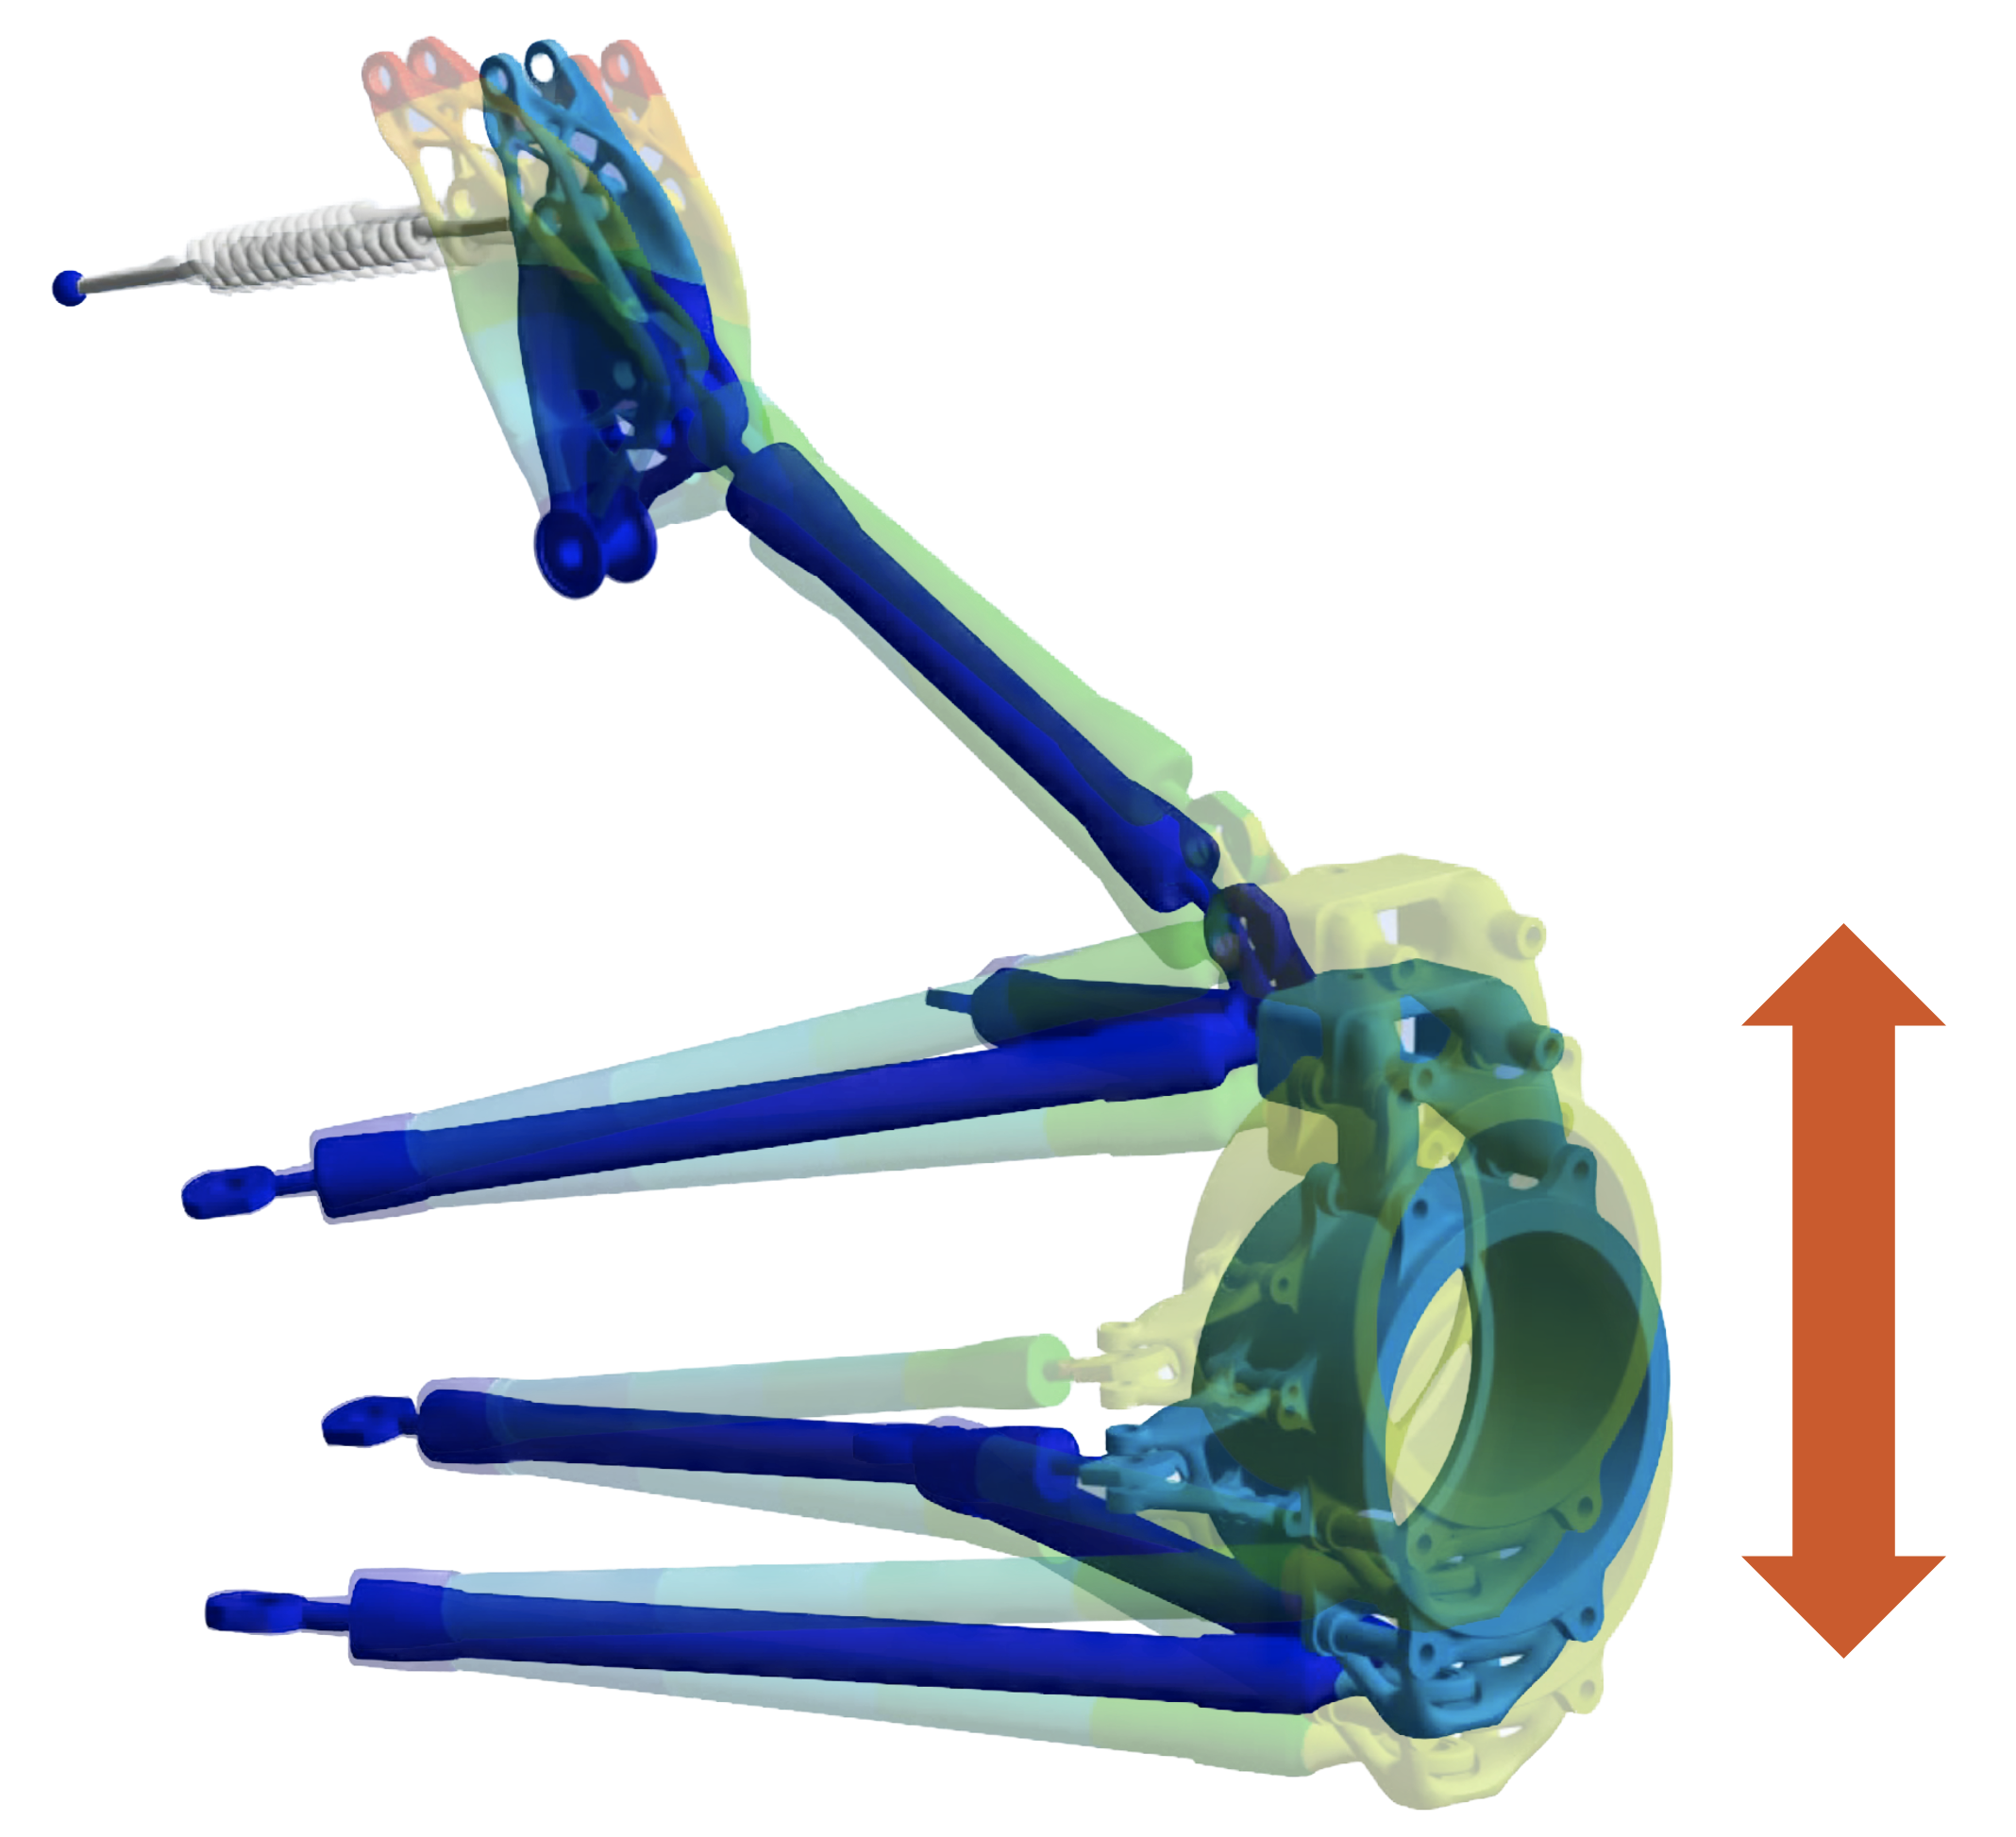
\includegraphics[width=1.0\linewidth]{figures/chapter_4/suspension_mode_1}
    \caption{$f_1 = \SSI{7.6}{\hertz}$}
  \end{subfigure}
  \begin{subfigure}[c]{0.225\textwidth}
    \centering
    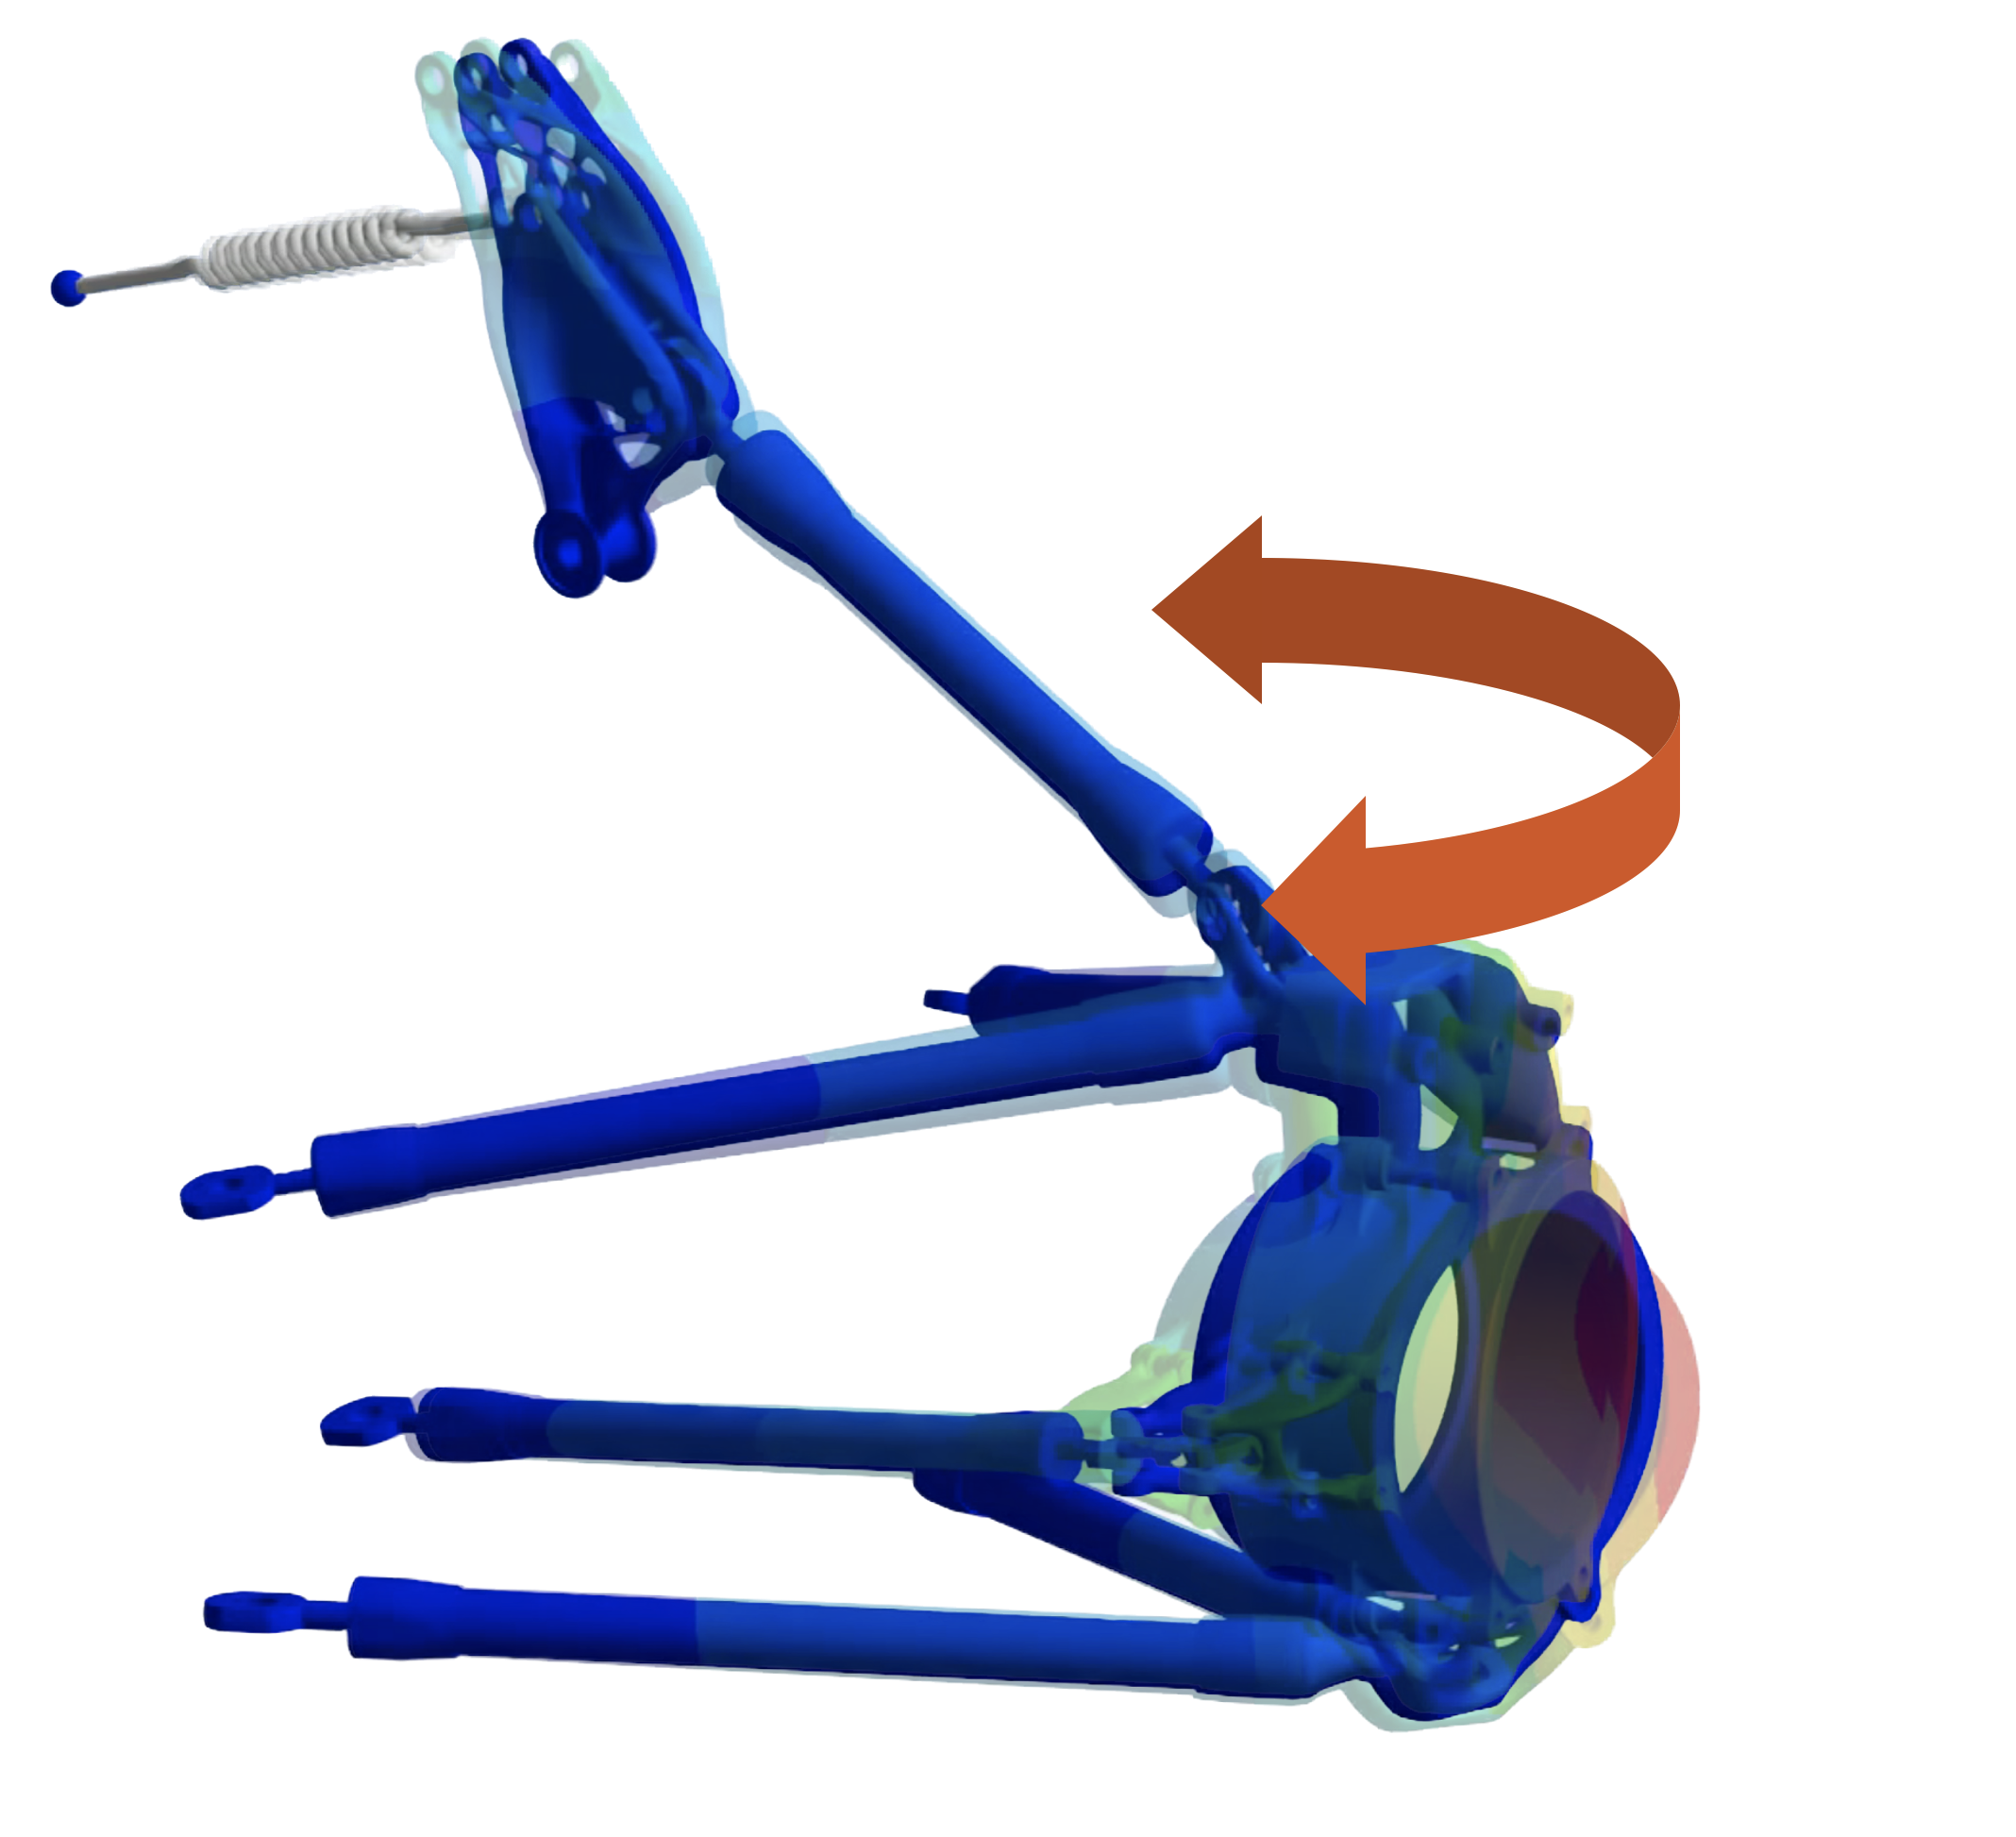
\includegraphics[width=1.0\linewidth]{figures/chapter_4/suspension_mode_2}
    \caption{$f_2 = \SSI{88.5}{\hertz}$}
  \end{subfigure}
  \begin{subfigure}[c]{0.225\textwidth}
    \centering
    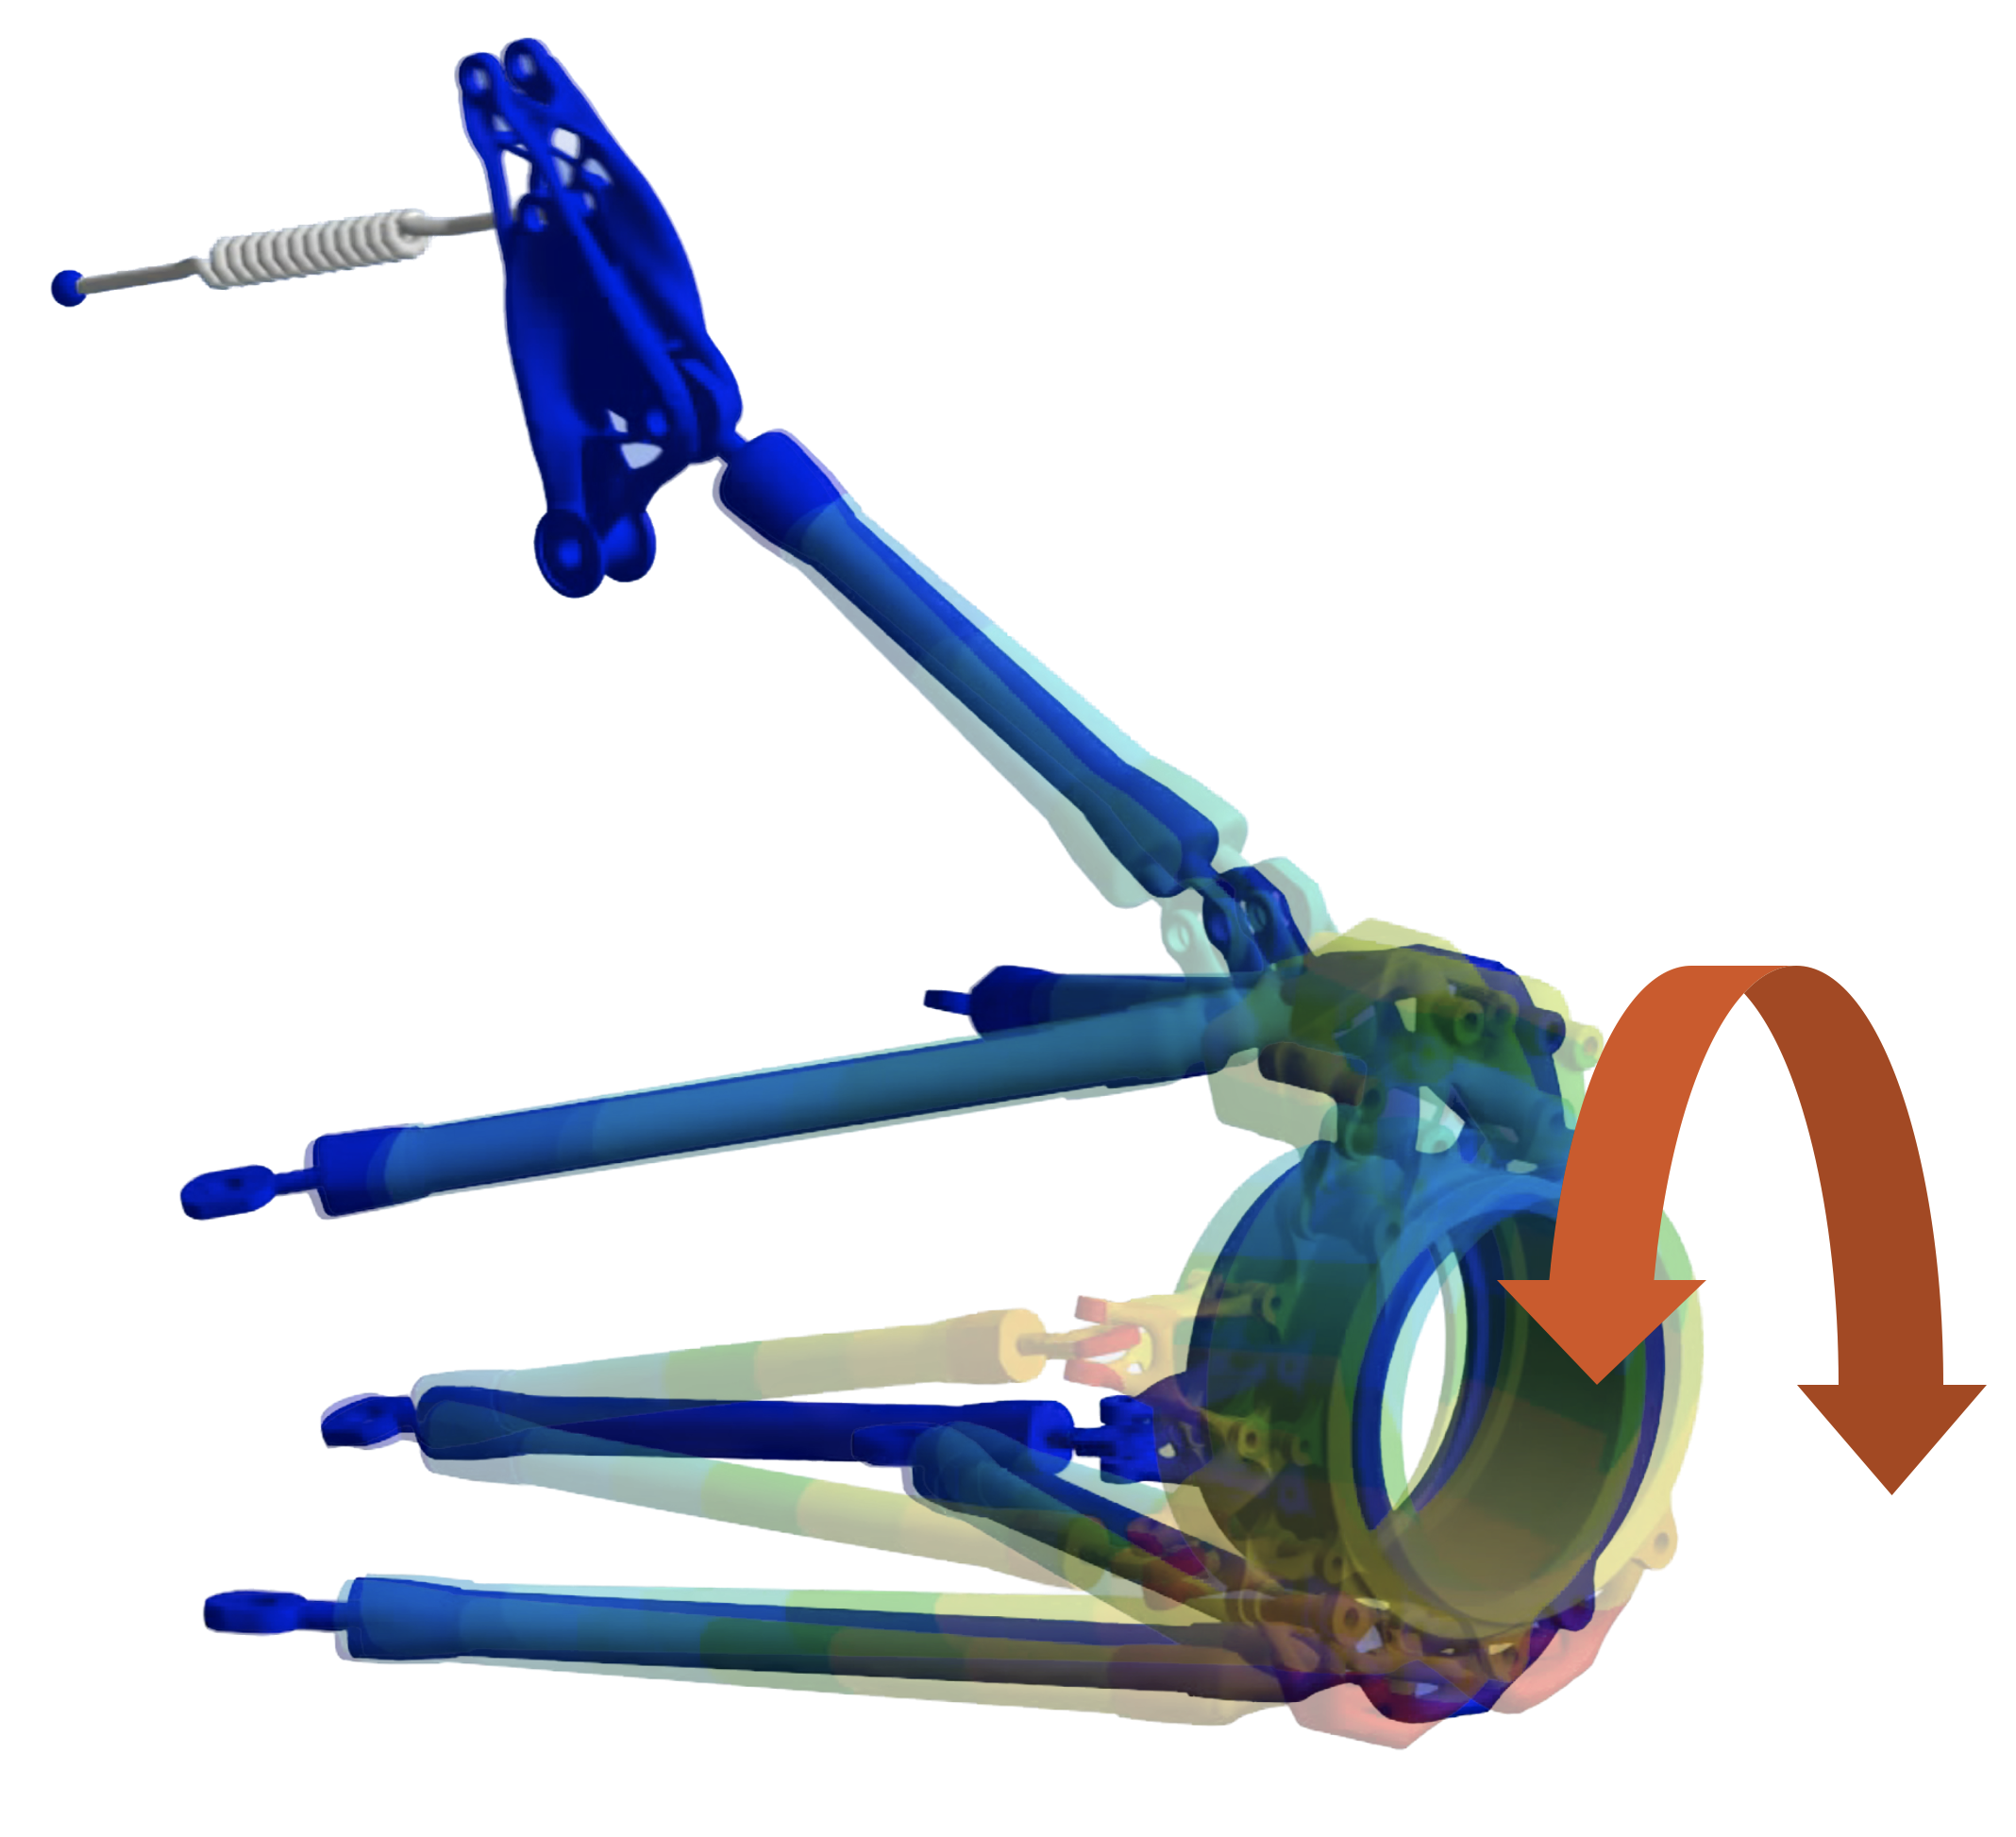
\includegraphics[width=1.0\linewidth]{figures/chapter_4/suspension_mode_3}
    \caption{$f_3 = \SSI{159.7}{\hertz}$}
  \end{subfigure}
  \caption{First three modal shapes of the suspension.}
  \label{chap4:fig:suspension_modes}
\end{figure}

\begin{figure}[htbp]
  \centering
  \small{\includetikz{figures/chapter_4/suspension_dynamic_deformations.tex}}
  \caption{Frequency response analysis of the suspension model is conducted, with tests performed under the equilibrium between the suspension system and a vertical force of \SI{500}{\newton} applied at the wheel hub. Frequency responses are assessed by applying input forces/torques at the wheel hub in the form of a linear chirp spanning frequencies from \SIrange{0}{200}{\hertz}, with a constant amplitude of \SI{5}{\newton}/\SI{5}{\newton\meter}. \emph{Legend:} {\color{mycolor1}$\blacksquare$} \Simulink{} multi-body simulation with full compliance dynamics contribution, {\color{mycolor2}$\blacksquare$} \Simulink{} multi-body with steady-state compliance contribution, {\color{mycolor3}$\blacksquare$} \Ansys{} \ac{FE} modal analysis.}
  \label{chap4:fig:suspension_dynamic_results}
\end{figure}

Finally, the reduced system is used to perform a transient analysis of the suspension system, coupled with the tire-ground enveloping model and the tire model presented in Appendix~\ref{app2:enve} (supported by the \Acme{} \cpp{} library described in Appendix~\ref{app1:acme}) and Appendix~\ref{app3:tirex}, respectively. The transient analysis is conducted to understand the impact of compliance on the system dynamics as well as suspension rods' diameter in the development of tire-ground forces. A side slip angle ramp simulation is thus performed to evaluate the effect of suspension compliance on the lateral force of the tire. For this simulation, the following four cases are analyzed:
%
\begin{itemize}
  \setlength\itemsep{0.0em}
  \item pure kinematic suspension model;
  \item kinematic and nominal compliance model;
  \item kinematic and compliance model with $-10\%$ suspension rods diameter;
  \item kinematic and compliance model with $-20\%$ suspension rods diameter.
\end{itemize}
%
The results of the simulation are shown in \figurename~\ref{chap4:fig:test_bench}, which compares the four cases. The lateral force $F_y$ is depicted with solid lines, while the difference between the lateral force of the pure kinematic simulation and the other cases is illustrated in dashed lines. The displayed curves show a non-negligible effect of suspension compliance on the lateral force of the tire is observed. As expected, the larger difference in the generated $F_y$ force can be observed in the linear region of the tire slip characteristic curve, where the slip cornering stiffness is higher. The difference then decreases as the peak approaches. Further observations could be made on the impact of these findings on the vehicle dynamics and handling. However, this is beyond the scope of this work.

\begin{figure}[!htp]
  \centering
  \small{\includetikz{figures/chapter_4//test_bench.tex}}
  \caption{Tire lateral force $F_y$ during a side slip angle ramp simulation. Solid lines represent the results obtained with the \Simulink{} model, while dashed lines represent the difference between the various simulations (see legend below). \emph{Solid lines legend:}
  {\color{mycolor1}\raisebox{-.15pt}{$\blacksquare$}} kinematics, {\color{mycolor2}\raisebox{-.15pt}{$\blacksquare$}} kinematics and compliance, {\color{mycolor3}\raisebox{-.15pt}{$\blacksquare$}} kinematics and compliance ($-10\%$ rods diameter), {\color{mycolor5}\raisebox{-.15pt}{$\blacksquare$}} kinematics and compliance ($-20\%$ rods diameter).   \emph{Dashed lines legend:} {\color{mycolor1}\raisebox{-.15pt}{\scalebox{0.5}[1.0]{$\blacksquare$}}}{\color{mycolor2}\raisebox{-.15pt}{\scalebox{0.5}[1.0]{$\blacksquare$}}} = {\color{mycolor1}\raisebox{-.15pt}{$\blacksquare$}} $-$ {\color{mycolor2}\raisebox{-.15pt}{$\blacksquare$}}, {\color{mycolor1}\raisebox{-.15pt}{\scalebox{0.5}[1.0]{$\blacksquare$}}}{\color{mycolor3}\raisebox{-.15pt}{\scalebox{0.5}[1.0]{$\blacksquare$}}} = {\color{mycolor1}\raisebox{-.15pt}{$\blacksquare$}} $-$ {\color{mycolor3}\raisebox{-.15pt}{$\blacksquare$}},  {\color{mycolor1}\raisebox{-.15pt}{\scalebox{0.5}[1.0]{$\blacksquare$}}}{\color{mycolor5}\raisebox{-.15pt}{\scalebox{0.5}[1.0]{$\blacksquare$}}} = {\color{mycolor1}\raisebox{-.15pt}{$\blacksquare$}} $-$ {\color{mycolor5}\raisebox{-.15pt}{$\blacksquare$}}.
  }
  \label{chap4:fig:test_bench}
\end{figure}

\section{Trajectory Prescribed Path Control}
\label{chap4:sec:tppc}

The \ac{TPPC} category is characterized by \ac{DAE} systems that describe the motion of a dynamical system whose trajectory is prescribed by adding a set of path constraints to the equations of motion. The model equations evolve into a non-linear semi-explicit \acp{DAE}. Within this system, the differential equations represent motion equations, while the algebraic equations correspond to imposed path constraints, collectively constituting \ac{TPPC} problems. Historically, addressing specific \ac{TPPC} challenges involved the development of software models that promptly adjust control variables to approximate prescribed path profiles. In this context, we investigate general numerical techniques directly applicable to \acp{DAE}. \ac{TPPC} problems are present in various fields, such as robot control, chemical process management, as well as space vehicle and aircraft guidance.

The \ac{DAE} systems arising from \ac{TPPC} simulations has typically the Hessenberg form~\cite{brenan1986numerical}
%
\begin{equation*}
  \begin{cases}
    \m{x}^\prime = \m{f}(\m{x}, \m{u}, t) & \text{differential equations} \\
    \m{0}        = \m{g}(\m{x}, \m{u}, t) & \text{path constraints}
  \end{cases} \, \text{,}
  \quad \text{with} \quad \jac{\m{g}}{\m{x}} \, \jac{\m{f}}{\m{u}} ~ \text{non-singular}
  \label{chap4:eq:tppc_dae_index2}
\end{equation*}
%
for index-2 problems, and
%
\begin{equation*}
  \begin{cases}
    \m{x}^\prime = \m{f}(\m{x}, \m{y}, \m{u}, t) \\
    \m{y}^\prime = \m{g}(\m{x}, \m{y}, t) \\
    \m{0}        = \m{h}(\m{y}, t)
  \end{cases} \, \text{,}
  \quad \text{with} \quad \jac{\m{h}}{\m{y}} \, \jac{\m{g}}{\m{x}} \, \jac{\m{f}}{\m{u}} ~ \text{non-singular}
  \label{chap4:eq:tppc_dae_index3}
\end{equation*}
%
for index-3 problems. The index of such systems is typically higher than the non-controlled counterpart. Indeed, the path constraints control is embedded in the state equations, often increasing the length of the differentiation chain to obtain a set of \acp{ODE}. Specifically, when the Jacobian $\jac{\m{g}}{\m{u}}$ is non-singular, the path equations are commonly referred to as control variable constraints and the corresponding \acp{DAE} has index-1. It is not uncommon to find that the path constraints in a \ac{TPPC} problem are functions only of the differential variables so that $\jac{\m{g}}{\m{u}} = \m{0}$ and the \acp{DAE} will be of higher index~\cite{brenan1995numerical}. To showcase the capabilities of the proposed index reduction algorithm in handling such high index \ac{TPPC} problems, different examples are presented. Two problems regarding the initial and final phases of the space shuttle reentry, described by index-2 and index-3 \acp{DAE}~\cite{brenan1995numerical}. Lastly, one problem on the control of a robotic arm, which is described as an index-5 system~\cite{pryce1998solving}. A brief discussion of each of these examples, together with an introduction to the application field, is presented in the following sections.

\subsection{Space Shuttle Reentry Problems}

In space applications, \ac{TPPC} problems aid in vehicle performance analysis during design, particularly for lifting reentry vehicles aiming to determine maximum crossrange (or downrange) capability. Trajectory profiles are constrained by skin temperature limits set by the thermal protection design. \ac{OC} theory offers a direct approach to addressing maximum crossrange capability with heating constraints, formulated as a \ac{TP-BVP} involving \acp{DAE} and adjoint variables. However, solving such \acp{OCP} requires starting solutions close to the optimal, especially with heating constraints, due to extreme sensitivity to initial guesses in shooting problems. An indirect \ac{TPPC} approach or using \ac{TPPC} to generate initial solutions for \ac{OC} may offer more success. Typically, maximizing crossrange capability involves holding the angle of attack $\alpha$ near the maximum lift/drag value, often set at around \SI{40}{\deg} in \ac{NASA} space shuttle reentry simulations, leaving bank angle $\beta$ adjustments to satisfy remaining functional constraints. In certain scenarios, varying system parameters can effectively optimize vehicle crossrange capability by ensuring trajectory adherence to specific constraints, thereby presenting a semi-explicit non-linear \acp{DAE} \ac{TPPC} problem~\cite{brenan1986numerical, brenan1995numerical}.

The discussion is confined to a reentry vehicle in the absence of propulsive forces, where we simplify the simulation to model solely spherical geopotential and spherical earth. The equations of motion in relative coordinates are thus expressed as follows
%
\begin{equation}
  \begin{cases}
  H^{\prime}       = V_r\sin(\gamma) \\
  \xi^{\prime}     = \dfrac{V_r\cos(\gamma) \sin(A)}{r \cos(\lambda)} \\
  \lambda^{\prime} = \dfrac{V_r}{r} \cos(\gamma) \cos(A) \\
  V_r^{\prime}     = -\dfrac{D}{m} - g\sin(\gamma) - \Omega_e^2 r \cos(\lambda)(\sin(\lambda) \cos(A) \cos(\gamma)-\cos(\lambda) \sin(\gamma)) \\
  \gamma^{\prime}  = \dfrac{L\cos(\beta)}{m V_r}+\dfrac{\cos(\gamma)}{V_r}\left(\dfrac{V_r^2}{r}-g\right) + 2\Omega_e \cos(\lambda) \sin(A)\dots \\
  \qquad + \dfrac{\Omega_e^2 r \cos(\lambda)}{V_r}(\sin(\lambda) \cos(A) \sin(\gamma)+\cos(\lambda) \cos(\gamma)) \\
  A^{\prime}       = \dfrac{L\sin(\beta)}{m V_r \cos(\gamma)}+\dfrac{V_r}{r} \cos(\gamma) \sin(A) \tan(\lambda) - 2\Omega_e(\cos(\lambda) \cos(A) \tan(\gamma) - \sin(\lambda)) \dots \\
  \qquad + \dfrac{\Omega_e^2 r \cos(\lambda) \sin(\lambda) \sin(A)}{V_r \cos(\gamma)}
  \end{cases} \, \text{,}
  \label{chap4:eq:space_shuttle_reentry}
\end{equation}
%
where the state variables are $\m{x} = [H, \xi, \lambda, V_r, \gamma, A]^\top$. The parameters are the following
%
\begin{equation*}
  \begin{aligned}
    r           & = H + r_e, & \text{distance from the earth center,} \\
    r_e         & = \SI{20902900}{\feet} & \text{earth radius,} \\
    g           & = \mu/r^2 & \text{gravity force,} \\
    \mu         & = \SI{1.407653916\times 10^16}{\cubic\feet\per\second\squared} & \text{gravitational constant,} \\
    \Omega_e    & = \SI{360/(24\cdot60\cdot60)}{\deg\per\second} & \text{earth angular speed,} \\
    \rho(H)     & = 0.002378\exp(-H/23800) & \text{atmospheric density,} \\
    L(V_r)      & = 1/2 \rho C_L S V_r^2 & \text{aerodynamic lift force,} \\
    D(V_r)      & = 1/2 \rho C_D S V_r^2 & \text{aerodynamic drag force.}
  \end{aligned}
\end{equation*}
%
The aerodynamic lift and drag coefficients, respectively $C_L(\alpha)$ and $C_D(\alpha)$, as well as the vehicle cross-sectional area $S$ and mass $m$, will be later specified on the specific test. The control variables, which dictate both the magnitude and direction of the aerodynamic force applied to the vehicle, are assessed within the body coordinate system (refer to \figurename~\ref{chap4:fig:shuttle_frame}). The bank angle $\beta$ corresponds to a rotation or \emph{roll} about the vehicle's $x$-axis, while the angle of attack $\alpha$ is measured from the relative velocity vector of the vehicle to the body $x$-axis, representing a rotation or \emph{pitch} about the body $y$-axis. For a more detailed explanation of these parameters and the coordinate system on the presented tests, please refer to~\cite{brenan1983stability}. Nonetheless, figure~\ref{chap4:fig:shuttle_reentry} illustrates the space shuttle coordinate system, as well as the vehicle's position with respect to the earth reference frame.

\begin{figure}[htb]
  \centering
  \begin{subfigure}[c]{0.475\textwidth}
    \centering
    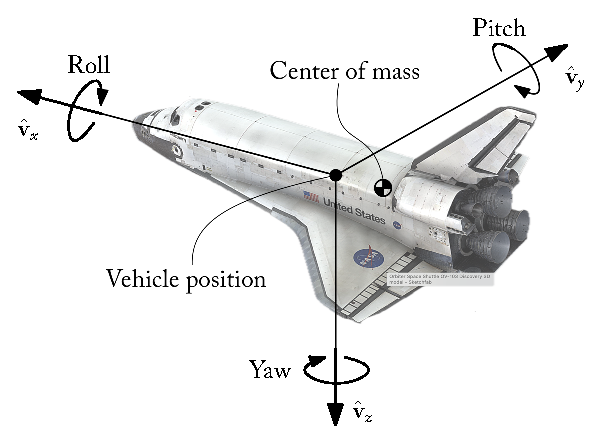
\includegraphics[width=1.0\linewidth]{figures/chapter_4/shuttle_frame.eps}
    \caption{Space shuttle reentry vehicle coordinate system.}
    \label{chap4:fig:shuttle_frame}
  \end{subfigure}%
  \hfill
  \begin{subfigure}[c]{0.475\textwidth}
    \centering
    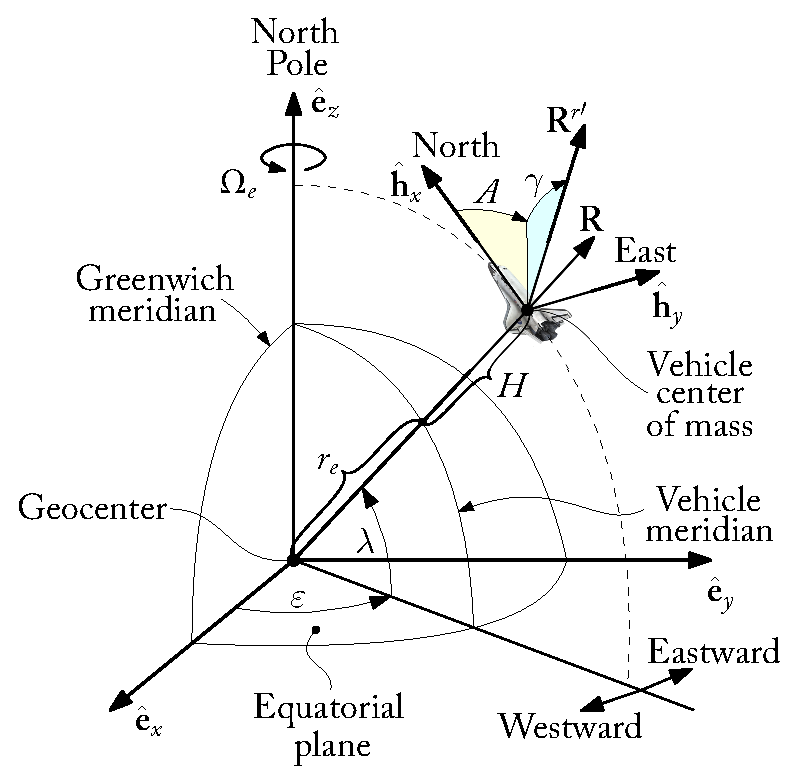
\includegraphics[width=1.0\linewidth]{figures/chapter_4/earth_frame.eps}
    \caption{Earth reference frame.}
    \label{chap4:fig:earth_frame}
  \end{subfigure}
  \caption{Coordinate systems for the space shuttle reentry problem~\cite{brenan1995numerical, brenan1986numerical}.}
  \label{chap4:fig:shuttle_reentry}
\end{figure}

Once the space shuttle concludes its mission in space, it must return to Earth for landing, subject to various mission constraints, such as heating limitations to prevent vehicle damage. Instead of directly imposing these heating constraints as algebraic limitations, an alternative approach involves prescribing a nominal drag acceleration versus a relative velocity profile. This profile is selected to ensure that temperature constraints are satisfied as long as the vehicle follows a trajectory complying with this drag constraint. During reentry, the standard equations of motion~\eqref{chap4:eq:space_shuttle_reentry} are compounded with an algebraic constraint representing the drag acceleration profile, forming a \ac{DAE} system. Typically, the angle of attack remains constant or is only slightly varied, while the bank angle serves as the control variable. In the following, we examine the initial and final phases of reentry. The first involves maneuvering the vehicle from a given state to one lying on the nominal drag constraint. While the second entails flying the vehicle along the nominal drag constraint.

\subsubsection{Initial Stage Reentry Problem}

We now examine the initial stage reentry \ac{TPPC} problem in the same form of~\cite{brenan1986numerical}. This problem is part of a broader trajectory optimization process aimed at determining a surface of admissible reentry states. Following completion of on-orbit maneuvers, the vehicle must transition to a state vector enabling safe flight to the landing site. This set of allowable states is denoted as a target line. A given initial state qualifies as a target line point if a trajectory can be executed from that state in such a way that the vehicle's drag versus relative velocity profile smoothly aligns with the specified nominal profile, without overshooting and thus without violating any temperature constraints. Consider now the description of the vehicle's drag acceleration versus relative velocity profile, expressed as
%
\begin{equation}
  \dfrac{D}{m} - (C_0 + C_1 (V_r - V_0) + C_2 (V_r - V_0)^2 + C_3 (V_r - V_0)^3) = 0 \, \text{,}
  \label{chap4:eq:initial_drag}
\end{equation}
%
for a time $t \in [t_0, t_1] = \RSI{32.868734542}{419.868734542}{\second}$, and where $V_0$, is the vehicle's initial velocity at $t_0$ and $C_0 = 3.974960446019$, $C_1 = -0.01448947694635$, $C_2 = -0.2156171551995 \cdot 10^{-4}$, and $C_3 = -0.1089609507291 \cdot 10^{-7}$ are constants chosen so that the initial state vector satisfies~\eqref{chap4:eq:initial_drag} and its first derivative at $t_0$, and so that this transitional phase smoothly joins with the nominal profile. Notice that, posed in this way, the resulting \ac{TPPC} system is a semi-explicit index-3 \acp{DAE} problem. In this test, the set of initial values are $\gamma = \SI{-0.749986488}{\deg}$, $A = \SI{62.7883367}{\deg}$, $H = \SI{264039.3280}{\feet}$, $\xi = \SI{177.718047}{\deg}$, $\lambda = \SI{32.0417885}{\deg}$, $V_r = \SI{24317.0798}{\feet\per\second}$, and $\beta = \SI{41.10071834}{\deg}$. The lift and drag coefficients $C_L = 0.8769230769$ and $C_D = 0.8246153846$, as well as the angle of attack $\alpha = \SI{40}{\deg}$ are assumed to be constant throughout the simulation. The vehicle mass is $m = \SI{5964.496499824}{\slugs}$, and its cross-sectional reference area is $S = \SI{2690}{\feet\squared}$.

\begin{table}
  \caption{Expression complexity encountered throughout the index reduction of the initial stage space shuttle reentry problem~\cite{brenan1995numerical} \ac{DAE} system index reduction. \emph{Legend}: $\cf$ = functions, $\ca$ = additions, $\cm$ = multiplications, and $\cd$ = divisions.}
  \label{chap4:tab:tppc_initial}
  \centering
  {\footnotesize\begin{tabular}{cccc}
    \multicolumn{4}{c}{\textbf{Initial Stage Space Shuttle Reentry Problem~\cite{brenan1995numerical}}} \\
    \toprule
    \textbf{Original \acp{DAE}} & \multicolumn{3}{c}{$\mF = 153\cf + 2\cd + 275\cm + 59\ca$ \quad $\mh = 0$} \\
    \midrule
    \textbf{Reduction step} & $\mE$ & $\mg$ & $\ma$ \\
    \midrule
    Index-3 \acp{DAE} & $11\cf + 9\cm + 5\ca$ & $118\cf + 1\cd + 220\cm + 36\ca$ & $6\cf + 1\cd + 28\cm + 10\ca$ \\
    Index-2 \acp{DAE} & $11\cf + 9\cm + 5\ca$ & $118\cf + 1\cd + 220\cm + 36\ca$ & $81\cf + 2\cd + 472\cm + 87\ca$ \\
    Index-1 \acp{DAE} & $11\cf + 9\cm + 5\ca$ & $118\cf + 1\cd + 220\cm + 36\ca$ & $567\cf + 3\cd + 6198\cm + 888\ca$ \\
    Index-0 \acp{DAE} & $4053\cf + 24\cd + 41102\cm + 5792\ca$ & $118\cf + 1\cd + 220\cm + 36\ca$ & $0$ \\
    \midrule
    \textbf{Reduced \acp{DAE}} & \multicolumn{3}{c}{$\mF = 3075\cf + 4\cd + 34811\cm + 4734\ca$ \quad $\mh = 654\cf + 6\cd + 6698\cm + 985\ca$} \\
    \bottomrule
  \end{tabular}}
\end{table}

To address this index-3 \acp{DAE}, we utilize the proposed index reduction algorithm. The complexity of expressions encountered during the algorithm's execution is detailed in Table~\ref{chap4:tab:tppc_initial}. Notably, the index reduction algorithm effectively reduced the system to index-0 without introducing any additional variables, and the expression growth is inhibited by successful simplification. We conduct numerical integration of the reduced \ac{DAE} system using both the \Maple{} and \Indigo{} solvers. \Maple{} encounters challenges in integrating the original \ac{DAE} system due to difficulties in projecting initial values into the solution space, where initial conditions are deemed inconsistent with the algebraic constraints. In contrast, the \Indigo{} numerical solver successfully integrates the reduced \ac{DAE} system, yielding results depicted in \figurename~\ref{chap4:fig:tppc_initial}.

\begin{figure}[htb]
  \centering
  \small{\includetikz{figures/chapter_4/shuttle_index3_control.tex}}
  \caption{Control history of the initial stage space shuttle reentry problem~\cite{brenan1995numerical}. The vehicle's trajectory is prescribed by the drag acceleration $D/m$ versus a relative velocity $V_r$ profile reported in~\eqref{chap4:eq:initial_drag}. The vehicle's state is controlled by the bank angle $\beta$ and the angle of attack is kept fix at $\alpha = \SI{40}{\deg}$. \emph{Legend}: \textcolor{mycolor1}{$\blacksquare$} bank angle $\beta$, and \textcolor{mycolor2}{$\blacksquare$} angle of attack $\alpha$.}
  \label{chap4:fig:tppc_initial}
\end{figure}

\subsubsection{Final Stage Reentry Problem}

We now examine the standard final stage reentry \ac{TPPC} problem in the same form of~\cite{brenan1995numerical}. Let's assume the objective is to navigate a vehicle along a predetermined azimuth $A$ and flight path angle trajectory $\gamma$, as defined by the constraints on state variables
%
\begin{equation}
  \gamma + 1 + 9\left(\dfrac{t}{300}\right)^2 = 0 \, \text{,}
  \qquad \text{and} \qquad
  A - 45 + 90\left(\dfrac{t}{300}\right)^2 = 0 \, \text{.}
  \label{chap4:eq:final_path_constraints}
\end{equation}
%
for a time $t \in \RSI{0}{300}{\second}$. The flight path angle $\gamma$ spans from $\RSI{-1}{-10}{\deg}$, while the azimuth $A$ ranges from $\RSI{45}{135}{\deg}$. Both the bank angle $\beta$ and the angle of attack $\alpha$ serve as control variables, \ie{} $\m{u} = [\beta, \alpha]^\top$. The \ac{DAE} system is index-2 for a lifting reentry vehicle as long as $(0.05 \rho S V_r/m)^2 C_L(\alpha)/\cos(\gamma) \neq 0$. Notice that to be physically consistent we require that $V_r \neq \SI{0}{\deg}$, $\rho\neq \SI{0}{\deg}$, $\alpha \neq \SI{0}{\deg}$, $\gamma \neq \SI{90}{\deg}$, as well as $\lambda \neq \SI{180}{\deg}$. The related index-1 \acp{DAE} can be obtained directly by differentiating the algebraic constraints once and substituting for $A^\prime$ and $\gamma^\prime$ from the differential equations. Consistent initial values for the \ac{DAE} system are determined by selecting the initial differential and control variables to satisfy~\eqref{chap4:eq:final_path_constraints} the two new hidden constraints in the related index-1 system. The set of initial values used in this experiment are $H = \SI{100000}{\feet}$, $\xi = \SI{0}{\deg}$, $\lambda = \SI{0}{\deg}$, $A = \SI{0}{\deg}$, $V_r = \SI{12000}{\feet\per\second}$, $\gamma = \SI{-1}{\deg}$, $A = \SI{45}{\deg}$, $\beta = \SI{-0.05220958616134}{\deg}$, and $\alpha = \SI{2.6728700742}{\deg}$. The lift and drag coefficients are set to $C_L = 0.01\alpha$ and $C_D = 0.04 + 0.1C_L^2$, respectively. The vehicle mass is $m = \SI{2.890532728}{\slugs}$, and its cross-sectional reference area is $S = \SI{1}{\feet\squared}$.

\begin{table}
  \caption{Expression complexity encountered throughout the index reduction of the final stage space shuttle reentry problem~\cite{brenan1995numerical} \ac{DAE} system index reduction. \emph{Legend}: $\cf$ = functions, $\ca$ = additions, $\cm$ = multiplications, and $\cd$ = divisions.}
  \label{chap4:tab:tppc_final}
  \centering
  {\footnotesize\begin{tabular}{cccc}
    \multicolumn{4}{c}{\textbf{Final Stage Space Shuttle Reentry Problem~\cite{brenan1995numerical}}} \\
    \toprule
    \textbf{Original \acp{DAE}} & \multicolumn{3}{c}{$\mF = 157\cf + 1\cd + 272\cm + 56\ca$ \quad $\mh = 0$} \\
    \midrule
    \textbf{Reduction step} & $\mE$ & $\mg$ & $\ma$ \\
    \midrule
    Index-2 \acp{DAE} & $11\cf + 9\cm + 5\ca$ & $126\cf + 1\cd + 237\cm + 39\ca$ & $2\cf + 4\cm + 4\ca$ \\
    Index-1 \acp{DAE} & $5\cf + 3\cm + 3\ca$ & $43\cf + 89\cm + 14\ca$ & $92\cf + 1\cd + 173\cm + 30\ca$ \\
    Index-0 \acp{DAE} & $428\cf + 6\cd + 714\cm + 119\ca$ & $52\cf + 1\cd + 107\cm + 18\ca$ & $0$ \\
    \midrule
    \textbf{Reduced \acp{DAE}} & \multicolumn{3}{c}{$\mF = 425\cf + 1\cd + 742\cm + 138\ca$ \quad $\mh = 94\cf + 1\cd + 177\cm + 34\ca$} \\
    \bottomrule
  \end{tabular}}
\end{table}

To solve the index-2 \ac{DAE} system, we apply the proposed index reduction algorithm. The expression complexity encountered throughout the index reduction is reported in Table~\ref{chap4:tab:tppc_final}. As we can see, the index reduction algorithm successfully reduces the index of the \ac{DAE} system to index-0 with minimal expression swelling. The numerical integration of the reduced \ac{DAE} system is performed using both the \Maple{} and \Indigo{} numerical solvers. In this regard, \Maple{} is not able to integrate the original \ac{DAE} system due to the incapacity of projecting the initial values into the solution space (\ie{}, initial conditions are not judged to be consistent with the algebraic constraints). Conversely, the numerical integration of the reduced \ac{DAE} system using the \Indigo{} numerical solver is successful, and the results are presented in \figurename~\ref{chap4:fig:tppc_final}.

\begin{figure}[htb]
  \centering
  \small{\includetikz{figures/chapter_4/shuttle_index2_control.tex}}
  \caption{Controls history of the space shuttle reentry problem~\cite{brenan1995numerical} in the time interval $t \in \RSI{0}{300}{\second}$. \emph{Legend}: \textcolor{mycolor1}{$\blacksquare$} bank angle $\beta$, and \textcolor{mycolor2}{$\blacksquare$} angle of attack $\alpha$.}
  \label{chap4:fig:tppc_final}
\end{figure}

\subsection{Robot Arm Control}

Another example of a \ac{TPPC} problem is the control of a robot arm, described as an index-5 \ac{DAE} system~\cite{pryce1998solving}. The system describes the path control of a two-link, flexible joint, planar robotic arm from~\cite{campbell1988general}. This system, which is frequently used in \acp{DAE} test case, is characterized by a high index, which is typical of \ac{TPPC} problems, as well as by the presence of various singularities~\cite{schwarz2020singularities}. The problem is a semi-explicit \acp{DAE} of dimension 8 with 2 path constraints. The system is described by the following equations The variables $[x_1, x_2, x_3]$ represent the angular coordinates of the end effector, while $[x_4, x_5, x_6]$ are their derivatives. The control variables are $[u_1, u_2]$, which represent the torques applied to the joints. The system is described by the following equations

\begin{equation}
  \begin{cases}
    x_1^{\prime} = x_4 \\
    x_2^{\prime} = x_5 \\
    x_3^{\prime} = x_6 \\
    x_4^{\prime} = 2c(x_3)(x_4+x_6)^2 - x_4^2d(x_3) - (2x_3-x_2)(a(x_3)+2b(x_3)) - a(x_3)(u_1-u_2) \\
    x_5^{\prime} = 2c(x_3)(x_4+x_6)^2 - x_4^2d(x_3) + (2 x_3-x_2)(1-3a(x_3)-2b(x_3)) - a(x_3)(u_1-u_2) + u_2 \\
    x_6^{\prime} = 2c(x_3)(x_4+x_6)^2 - x_4^2d(x_3) + (2 x_3-x_2)(a(x_3)-9b(x_3)) - (a(x_3)+b(x_3))(u_1-u_2) \dots \\
    \qquad - d(x_3)(x_4+x_6)^2 - 2x_4^2c(x_3) \\
    0 = \cos(x_1) + \cos(x_1+x_3) - p_1(t) \\
    0 = \sin(x_1) + \sin(x_1+x_3) - p_2(t)
  \end{cases} \, \text{,}
\end{equation}
%
with
%
\begin{equation}
  a(z) = \dfrac{2}{2-\cos(z)^2} \, \text{,}
  \quad
  b(z) = \dfrac{\cos(z)}{2-\cos(z)^2} \, \text{,}
  \quad
  c(z) = \dfrac{\sin(z)}{2-\cos(z)^2} \, \text{,}
  \quad \text{and} \quad
  d(z) = \dfrac{\cos(z)\sin(z)}{2-\cos(z)^2} \, \text{.}
\end{equation}
%
The end effector path constraints are given by
%
\begin{equation}
  p_1(t) = \cos(\exp(t) - 1) + \cos(t - 1) \, \text{,}
  \quad \text{and} \quad
  p_2(t) = \sin(1 - \exp(t)) + \sin(1 - t) \, \text{.}
\end{equation}
%
Figure~\ref{chap4:fig:robotic_arm} illustrates the robotic arm problem, as well as its variables and control parameters.

\begin{figure}[htb]
  \centering
  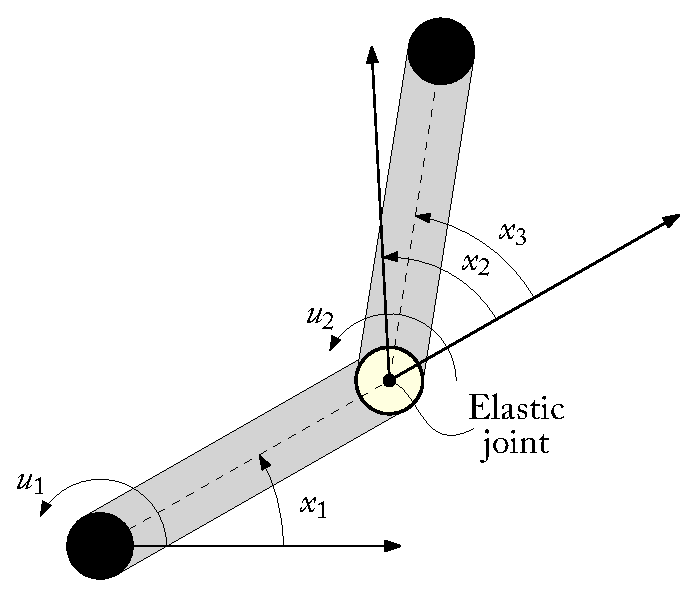
\includegraphics[width=0.4\linewidth]{figures/chapter_4/robotic_arm.eps}
  \caption{Robot arm control problem.}
  \label{chap4:fig:robotic_arm}
\end{figure}

\begin{table}
  \caption{Expression complexity encountered throughout the index reduction of the robotic arm problem~\cite{brenan1995numerical} \ac{DAE} system index reduction. \emph{Legend}: $\cf$ = functions, $\ca$ = additions, $\cm$ = multiplications, and $\cd$ = divisions.}
  \label{chap4:tab:tppc_robot}
  \centering
  \resizebox{\textwidth}{!}{%
  {\footnotesize\begin{tabular}{cccc}
    \multicolumn{4}{c}{\textbf{Robotic Arm~\cite{pryce1998solving}}} \\
    \toprule
    \textbf{Original \acp{DAE}} & \multicolumn{3}{c}{$\mF = 125\cf + 19\cd + 56\cm + 64\ca$ \quad $\mh = 0$} \\
    \midrule
    \textbf{Reduction step} & $\mE$ & $\mg$ & $\ma$ \\
    \midrule
    Index-5 \acp{DAE} & $0$ & $66\cf + 3\cd + 50\cm + 35\ca$ & $16\cf + 12\ca$ \\
    Index-4 \acp{DAE} & $0$ & $66\cf + 3\cd + 50\cm + 35\ca$ & $24\cf + 6\cm + 14\ca$ \\
    Index-3 \acp{DAE} & $0$ & $66\cf + 3\cd + 50\cm + 35\ca$ & $162\cf + 2\cd + 138\cm + 114\ca$ \\
    Index-2 \acp{DAE} & $14\cf + 2\cd + 6\cm + 6\ca$ & $372\cf + 4\cd + 375\cm + 253\ca$ & $972\cf + 1\cd + 1062\cm + 770\ca$ \\
    Index-1 \acp{DAE} & $14\cf + 2\cd + 6\cm + 6\ca$ & $372\cf + 4\cd + 375\cm + 253\ca$ & $\star (6.5\cf + 5.6\cm + 1.8\ca)\cdot10^{6} + 4\cd$ \\
    Index-0 \acp{DAE} & $\star (8.3\cf + 7.1\cm + 2.3\ca)\cdot10^{7} + 58\cd$ & $(2.4\cf + 2.0\cm + 0.9\ca)\cdot10^{6} + 8\cd$ & $0$ \\
    \midrule
    \textbf{Reduced \acp{DAE}} & \multicolumn{3}{c}{$\star \mF = (8.6\cf + 7.3\cm + 2.4\ca)\cdot10^{7} + 66\cd$ \quad $\star \mh = (6.5\cf + 5.6\cm + 1.8\ca)\cdot10^{6} + 7\cd$} \\
    \bottomrule
    \end{tabular}}
    }
\end{table}

\begin{table}
  \caption{Expression complexity encountered throughout the index reduction with the aid of hierarchical representation of the robotic arm problem~\cite{brenan1995numerical} \ac{DAE} system index reduction. \emph{Legend}: $\cf$ = functions, $\cv$ = veiling variables, $\ca$ = additions, $\cm$ = multiplications, and $\cd$ = divisions.}
  \label{chap4:tab:tppc_robot_veil}
  \centering
  {\footnotesize\begin{tabular}{cccc}
    \multicolumn{4}{c}{\textbf{Robotic Arm~\cite{pryce1998solving}}} \\
    \toprule
    \textbf{Original \acp{DAE}} & \multicolumn{3}{c}{$\mF = 125\cf + 19\cd + 56\cm + 64\ca$ \quad $\mh = 0$ \quad $\mv = 0$} \\
    \midrule
    \textbf{Reduction step} & $\mE$ & $\mg$ & $\ma$ \\
    \midrule
    Index-5 \acp{DAE} & $0$ & $66\cf + 3\cd + 50\cm + 35\ca$ & $16\cf + 12\ca$ \\
    Index-4 \acp{DAE} & $0$ & $66\cf + 3\cd + 50\cm + 35\ca$ & $24\cf + 6\cm + 14\ca$ \\
    Index-3 \acp{DAE} & $0$ & $66\cf + 3\cd + 50\cm + 35\ca$ & $162\cf + 2\cd + 138\cm + 114\ca$ \\
    Index-2 \acp{DAE} & $14\cf + 2\cd + 6\cm + 6\ca$ & $66\cf + 1\cv + 3\cd + 51\cm + 35\ca$ & $1\cm + 1\cv$ \\
    Index-1 \acp{DAE} & $2\cv + 1\ca$ & $66\cf + 1\cv + 3\cd + 51\cm + 35\ca$ & $9\cf + 4\cv + 2\cd + 8\cm + 5\ca$ \\
    Index-0 \acp{DAE} & $7\cv + 1\cd + 2\cm + 2\ca$ & $66\cf + 2\cv + 3\cd + 52\cm + 35\ca$ & $0$ \\
    \midrule
    \textbf{Reduced \acp{DAE}} & \multicolumn{3}{c}{$\mF = 90\cf + 9\cv + 4\cd + 63\cm + 48\ca$ \quad $\mh = 202\cf + 5\cv + 4\cd + 141\cm + 130\ca$} \\
    \bottomrule
  \end{tabular} \\[0.5em]
  \begin{tabular}{cc}
    \multicolumn{2}{c}{Hierarchical representation details (29 veils)} \\
    \toprule
    \textbf{Original \acp{DAE}} & $\mv = 0$ \\
    \midrule
    \textbf{Reduction step} & $\mv$ \\
    \midrule
    Index-5 \acp{DAE} & $0$ \\
    Index-4 \acp{DAE} & $0$ \\
    Index-3 \acp{DAE} & $0$ \\
    Index-2 \acp{DAE} & $1278\cf + 3\cv + 6\cd + 1319\cm + 918\ca$ \\
    Index-1 \acp{DAE} & $8401\cf + 20\cv + 24\cd + 9451\cm + 6095\ca$ \\
    Index-0 \acp{DAE} & $37010\cf + 558\cv + 56\cd + 45087\cm + 28665\ca$ \\
    \midrule
    \textbf{Reduced \acp{DAE}} & $\mv = 37010\cf + 558\cv + 56\cd + 45087\cm + 28665\ca$ \\
    \bottomrule
  \end{tabular}}
\end{table}

The complexity of expressions encountered throughout the index reduction is detailed in Table~\ref{chap4:tab:tppc_robot}. The index reduction algorithm effectively reduces the system to index-0 without introducing any additional variables, however, substantial expression growth is observed. The simplification of the expressions within \SI{100}{\second} of \ac{CPU} time is not feasible. Hierarchical representation through veiling variables is necessary to simplify the handling of the system expressions. The complexity of the expressions encountered throughout the index reduction with the aid of hierarchical representation is detailed in Table~\ref{chap4:tab:tppc_robot_veil}. The introduction of veiling variables effectively reduced the overall expression complexity by a factor of at least $10^4$. This can be attributed to the fact that the chunks of the system are now more efficiently handled by the \ac{CAS}, and simplification can be effectively performed. The numerical integration of the reduced \ac{DAE} system is performed using both the \Maple{} and \Indigo{} numerical solvers. In this regard, \Maple{} is not able to integrate the original \ac{DAE} system due to the incapacity of projecting the initial values into the solution space. Conversely, the numerical integration of the reduced \ac{DAE} system using the RadauIIA5 \Indigo{} numerical solver is successful in the interval $t \in \RSI{0}{0.98}{\second}$. It must be pointed out that this system presents many singularities that hinder a flawless integration (refer to~\cite{schwarz2020singularities} for a detailed analysis).

For what concerns \Mathematica{} and \Matlab{} performances, the tests we performed showed that both solvers are not able to integrate the original \ac{DAE} system due to the incapacity of projecting the initial values into the solution space. Furthermore, the Pantelides algorithm implemented in \Matlab{} is not able to reduce the index of the system to index-1.

\section{Electrical Circuits}
\label{chap4:sec:electrical_circuits}

Historically, the \acp{DAE} of electrical networks stimulated the study of \acp{DAE} and their solutions since the early 70s~\cite{gear1971simultaneous}. \acp{DAE} encountered in this domain exhibit a distinct structure, somewhat different from those arising from mechanical systems or \ac{TPPC}. Typically, these \acp{DAE} are large and sparse, often linear, although non-linearities may arise from certain circuit components. Our focus here is not to give a detailed account of circuit design, but rather to illustrate the types of \acp{DAE} that may arise and how various aspects of the circuit influence \ac{DAE} system properties such as index, solvability, and numerical solution.

Consider an electrical network comprising $b$ branches connected to $n$ nodes. Assigning a current variable $i_b$ to each branch and a voltage variable $v_n$ to each node, the circuit equations stem from Kirchoff's laws, \ie{} the algebraic sum of currents into a node is zero, and the algebraic sum of the voltage drops around a loop is zero. By convention, current denotes the net flow of positive charge, with a designated current direction along each branch assigned by designating one node as negative and the other as positive (with current flowing from positive to negative). The circuit's topology can be described by a $b \times n$ network incidence matrix $\m{A}$. The $(i,j)$ element of $\m{A}$ is $\pm1$ if node $j$ is the $\pm$ node for the $i$-th branch. Denoting $\m{i}_b$ as the vector of current variables, Kirchoff's current law simply states that $\m{A}^\top\m{i}_b$ = 0. The voltage drop across each branch is defined as the difference between the voltage at the positive node and that at the negative node. These branch voltages $\m{v}_b$ can be expressed in terms of the nodal voltages $\m{v}_n$ as $\m{v}_b = \m{A}\m{v}_n$.

Linear circuits composed of resistors, capacitors, and inductors can result in large sparse linear \acp{DAE}. In these circuits, the voltage-current relationship across a resistor branch follows Ohm's law, $v_r = Ri_r$, with a positive resistance $R$. Similarly, the voltage-current characteristics of linear capacitors and inductors satisfy $i_c = C\de{}v_c/\de{}t$ and $v_l = L\de{}i_l/\de{}t$, respectively. However, the inclusion of transistors or unicursal elements tends to introduce non-linearity into \ac{DAE} systems. The solvability of \acp{DAE} arising from linear circuits lacking operational amplifiers is solely influenced by the network topology. However, circuits containing differential amplifiers, typically realized using operational amplifiers, may give rise to \acp{DAE} of arbitrarily high index. \acp{DAE} arising from linear circuits incorporating operational amplifiers depends on the specific voltage-current characteristics of the circuit components for solvability. Moreover, the number of independent initial conditions may vary depending on specific circuit parameter values. The potential for arbitrarily high index \acp{DAE} originating from circuits is demonstrated in examples such as a cascade of differential amplifiers. Furthermore, high index \acp{DAE} may emerge when different variables are designated as inputs and outputs. For example, whether a device functions as a differentiator or an integrator depends on the designation of inputs and outputs~\cite{brenan1995numerical}.

In the following, we present three examples of electrical circuits, the first being an eight-node transistor-amplifier, the second an electric ring modulator, and the third a cascade of differential amplifiers. The first two examples are taken from~\cite{lioen1998test, mazzia2008test}, while the third is taken from~\cite{brenan1995numerical}.

\subsection{Eight-Node Transistor-Amplifier}

This problem originates from electrical circuit analysis. It is a model for the transistor amplifier. The diagram of the circuit is given in \figurename{}~\ref{chap4:fig:transistor_amplifier}. Here $U_e$ is the input signal and the amplified output signal can be found in point $8$. The circuit is described by a system of \acp{DAE} of index-1, consisting of 8 equations. The system is in the form $\m{M}\m{x}^\prime = \m{f}(\m{x},t)$, where $\m{x} = [x_1, \dots, x_8]^\top$, $\m{M}$ and $\m{f}(\m{x},t)$ being given by
%
\begin{equation}
  \m{M} = \begin{bmatrix}
    -C_1 & C_1 & 0 & 0 & 0 & 0 & 0 & 0 \\
    C_1 & -C_1 & 0 & 0 & 0 & 0 & 0 & 0 \\
    0 & 0 & -C_2 & 0 & 0 & 0 & 0 & 0 \\
    0 & 0 & 0 & -C_3 & C_3 & 0 & 0 & 0 \\
    0 & 0 & 0 & C_3 & -C_3 & 0 & 0 & 0 \\
    0 & 0 & 0 & 0 & 0 & -C_4 & 0 & 0 \\
    0 & 0 & 0 & 0 & 0 & 0 & -C_5 & C_5 \\
    0 & 0 & 0 & 0 & 0 & 0 & C_5 & -C_5
  \end{bmatrix} \, \text{,}
\end{equation}
%
\begin{equation}
  \m{f}(\m{x},t) = \begin{bmatrix}
    -\dfrac{U_e(t)}{R_0} + \dfrac{x_1}{R_0} \\
    -\dfrac{U_b}{R_2} + x_2\left(\dfrac{1}{R_1}+\dfrac{1}{R_2}\right) - (\alpha-1)g(x_2-x_3) \\
    -g(x_2-x_3)+\dfrac{x_3}{R_3} \\
    -\dfrac{U_b}{R_4} + \dfrac{x_4}{R_4} + \alpha g(x_2-x_3) \\
    -\dfrac{U_b}{R_6} + x_5\left(\dfrac{1}{R_5} + \dfrac{1}{R_6}\right)-(\alpha-1) g(x_5-x_6) \\
    -g(x_5-x_6) + \dfrac{x_6}{R_7} \\
    -\dfrac{U_b}{R_8} + \dfrac{x_7}{R_8} + \alpha g(x_5-x_6) \\
    \dfrac{x_8}{R_9}
  \end{bmatrix} \, \text{,}
\end{equation}
%
and $g(x) = \beta(\exp(x/U_f) - 1)\,\USI{\ampere}$, $U_e(t) = 0.1\sin(200 \pi t)\,\USI{\volt}$. Initial conditions at $t = 0$ and parameters are given by
%
\begin{equation*}
  \m{x}_0 = \begin{bmatrix}
    0 \\
    U_b/(R_2/R_1 + 1) \\
    U_b/(R_2/R_1 + 1) \\
    U_b \\
    U_b/(R_6/R_5 + 1) \\
    U_b/(R_6/R_5 + 1) \\
    U_b \\
    0 \\
  \end{bmatrix} \, \text{,}
  \qquad \text{and} \qquad
  \begin{array}{l}
    U_b = \SI{6}{\volt} \, \text{,} \\
    U_f = \SI{0.026}{\volt} \, \text{,} \\
    \alpha = 0.99 \, \text{,} \\
    \beta = \SI{10^-6}{\ampere} \, \text{,} \\
    R_0 = \SI{1}{\kilo\ohm} \, \text{,} \\
    R_k = \SI{9}{\kilo\ohm} ~ \text{with} ~ k=1, \dots, 9 \, \text{,} \\
    C_k = \SI{k}{\micro\farad} ~ \text{with} ~ k=1, \dots, 9 \, \text{.} \\
  \end{array} \, \text{.}
\end{equation*}

\begin{figure}
  \centering
  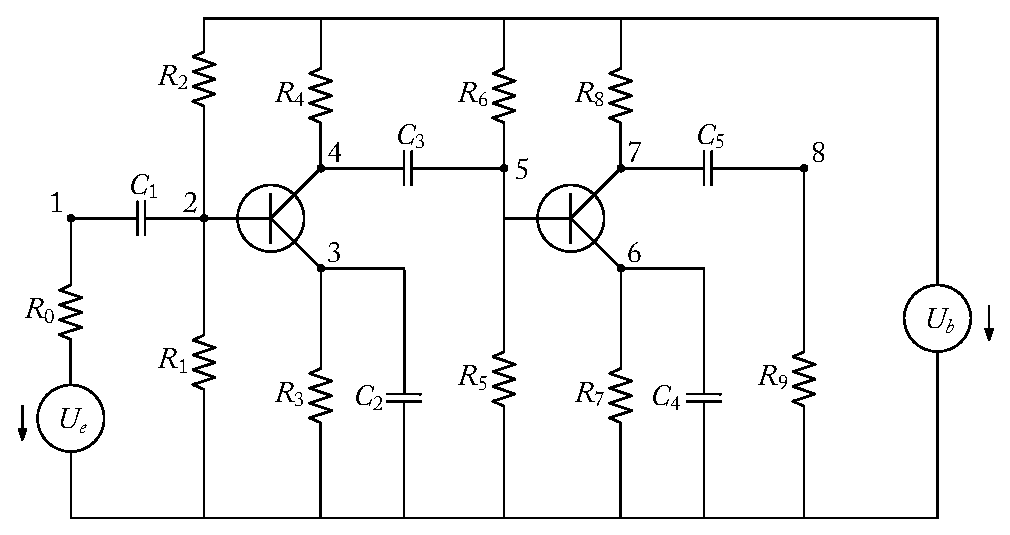
\includegraphics[width=0.7\textwidth]{figures/chapter_4/transistor_amplifier.eps}
  \caption{Eight-node transistor-amplifier circuit~\cite{lioen1998test, mazzia2008test}.}
  \label{chap4:fig:transistor_amplifier}
\end{figure}

The index reduction process is smoothly performed, and the complexity of the expressions encountered throughout the index reduction is detailed in Table~\ref{chap4:tab:tppc_robot}. As we can see, the expression complexity is minimally affected by the index reduction process. The numerical integration of the reduced \ac{DAE} system is performed using both the \Maple{} and \Indigo{} numerical solvers. In this regard, both \Maple{}, \Mathematica{}, \Matlab{} (both Pantelides and Gaussian elimination), and \Indigo{} can integrate the original \ac{DAE} system in the specified time interval $t \in \RSI{0}{0.2}{\second}$.

\begin{figure}[htb]
  \centering
  \small{\includetikz{figures/chapter_4/transistor_amplifier.tex}}
  \caption{Transistor amplifier circuit integration results~\cite{lioen1998test, mazzia2008test} in the time interval $t \in \RSI{0}{0.2}{\second}$. Notice that the output signal $U_8$ is equal to the state variable $x_8$. \emph{Legend}: \textcolor{mycolor1}{$\blacksquare$} input signal $U_e(t)$, and \textcolor{mycolor2}{$\blacksquare$} output signal $U_8$.}
  \label{chap4:fig:transistor_amplifier_results}
\end{figure}

\begin{table}
  \caption{Expression complexity encountered throughout the index reduction of the eight-node transistor-amplifier problem~\cite{lioen1998test, mazzia2008test} \ac{DAE} system index reduction. \emph{Legend}: $\cf$ = functions, $\ca$ = additions, $\cm$ = multiplications, and $\cd$ = divisions.}
  \label{chap4:tab:tppc_robot}
  \centering
  {\footnotesize\begin{tabular}{cccc}
    \multicolumn{4}{c}{\textbf{Eight-Nodes Transistor-Amplifier~\cite{lioen1998test, mazzia2008test}}} \\
    \toprule
    \textbf{Original \acp{DAE}} & \multicolumn{3}{c}{$\mF = 55\cf + 21\cd + 29\cm + 41\ca$ \quad $\mh = 0$} \\
    \midrule
    \textbf{Reduction step} & $\mE$ & $\mg$ & $\ma$ \\
    \midrule
    Index-1 \acp{DAE} & $5\ca$ & $17\cf + 11\cd + 22\cm + 20\ca$ & $19\cf + 12\cd + 44\cm + 24\ca$ \\
    Index-0 \acp{DAE} & $24\cf + 26\cd + 24\cm + 24\ca$ & $18\cf + 12\cd + 26\cm + 20\ca$ & $0$ \\
    \midrule
    \textbf{Reduced \acp{DAE}} & \multicolumn{3}{c}{$\mF = 74\cf + 26\cd + 87\cm + 49\ca$ \quad $\mh = 19\cf + 12\cd + 44\cm + 26\ca$} \\
    \bottomrule
    \end{tabular}}
\end{table}

\subsection{Electric Ring Modulator}

The electric ring modulator is an interesting example of a system whose structure depends on the specific values of the parameters. The system is in the form $\m{M}\m{x}^\prime = \m{f}(\m{x},t)$, where $\m{x} = [x_1, \dots, x_{15}]^\top$, $\m{M}$ and $\m{f}(\m{x},t)$ being given by
%
\begin{equation}
  \m{M} = \mathrm{diag}(C, C, C_s, C_s, C_s, C_s, C_p, L_h, L_h, L_{s2}, L_{s3}, L_{s2}, L_{s3}, L_{s1}, L_{s1}) \, \text{,}
\end{equation}
%
\begin{equation}
  \m{f}(\m{x},t) = \begin{bmatrix}
    x_8 - (x_{10} + x_{11})/2 + x_{14} - x_1/R \\
    x_9 - (x_{12} + x_{13})/2 + x_{15} - x_2/R \\
    x_{10} - q(U_{d1}) + q(U_{d4}) \\
    -x_{11} + q(U_{d2}) - q(U_{d3}) \\
    x_{12} + q(U_{d1}) - q(U_{d3}) \\
    -x_{13} - q(U_{d2}) + q(U_{d4}) \\
    -x_7/R_p + q(U_{d1}) + q(U_{d2}) - q(U_{d3}) - q(U_{d4}) \\
    x_1 \\
    x_2 \\
    x_1/2 - x_3 - R_{g2}x_{10} \\
    -x_1/2 + x_4 - R_{g3}x_{11} \\
    x_2/2 - x_5 - R_{g2}x_{12} \\
    -x_2/2 + x_6 - R_{g3}x_{13} \\
    -x_1 + U_{in1}(t) - (R_i + R_{g1})x_{14} \\
    -x_2 - (R_c+R_{g1})x_{15}
  \end{bmatrix} \, \text{,}
\end{equation}
%
where $U_{d1}, U_{d2}, U_{d3}, U_{d4}, q, U_{in1}$ and $U_{in2}$ are given by
%
\begin{equation}
  \begin{array}{l}
    U_{d1} = x_3 - x_5 - x_7 - U_{in2}(t) \, \text{,} \\
    U_{d2} = -x_4 + x_6 - x_7 - U_{in2}(t) \, \text{,} \\
    U_{d3} = x_4 + x_5 + x_7 + U_{in2}(t) \, \text{,} \\
    U_{d4} = -x_3 - x_6 + x_7 + U_{in2}(t) \, \text{,} \\
    q(U) = \gamma(exp(\delta U) - 1) \, \text{,} \\
    U_{in1}(t) = 1/2 \sin(2000 \pi t) \, \text{,} \\
    U_{in2}(t) = 2 \sin(20000 \pi t) \, \text{.}
  \end{array}
\end{equation}
%
Initial conditions at $t = 0$ and parameters are given by $\m{x}_0 = [0, 0, 0, 0, 0, 0, 0, 0, 0, 0, 0, 0, 0, 0, 0]^\top$, and
%
\begin{equation*}
  \begin{array}{l}
    C = \SI{16}{\nano\farad} \, \text{,} \\
    C_s = 0~\text{or}~\SI{2}{\pico\farad} \, \text{,} \\
    C_p = \SI{100}{\nano\farad} \, \text{,} \\
    L_h = \SI{4.45}{\henry} \, \text{,} \\
    L_{s1} = \SI{2}{\milli\henry} \, \text{,} \\
    L_{s2} = \SI{0.5}{\milli\henry} \, \text{,} \\
    L_{s3} = \SI{0.5}{\milli\henry} \, \text{,} \\
    \gamma = 40.67286402 \, \text{,} \\
  \end{array}
  \qquad
  \begin{array}{l}
    R = \SI{25}{\kilo\ohm} \, \text{,} \\
    R_p = \SI{50}{\ohm} \, \text{,} \\
    R_{g1} = \SI{36.3}{\ohm} \, \text{,} \\
    R_{g2} = \SI{17.3}{\ohm} \, \text{,} \\
    R_{g3} = \SI{17.3}{\ohm} \, \text{,} \\
    R_{i} = \SI{50}{\ohm} \, \text{,} \\
    R_{c} = \SI{600}{\ohm} \, \text{,} \\
    \delta = 17,7493332 \, \text{.} \\
  \end{array} \, \text{.}
\end{equation*}
%
It must be pointed out that if $C_s \neq 0$, the system is an \acp{ODE}, otherwise, it is an index-2 \ac{DAE} system. In the original test problem in~\cite{lioen1998test, mazzia2008test}, the authors set $C_s = \SI{2}{\pico\farad}$ to obtain an \ac{ODE} system. In Figure~\ref{chap4:fig:ring_modulator}, the electric ring modulator circuit is shown.

Considering $C_s = 0$, the index reduction process is flawlessly performed through the presented algorithm, complexity of the expressions encountered throughout the index reduction is detailed in Table~\ref{chap4:tab:tppc_robot}. Numerical integration in the specified time interval $t \in \RSI{0}{1}{\milli\second}$ is successfully performed by \Indigo{} numerical solvers. Conversely, \Maple{} is not able to integrate the original \ac{DAE} due to computational time exceeding \SI{100}{\second}. Results of the numerical integration are shown in Figure~\ref{chap4:fig:ring_modulator_results}, where the modulated output signal $U_2$ is represented. Notice that the modulated output signal is strongly influenced by the $C_s = 0$ assumption and the magnitude of $U_2$ is reduced by a factor of $10^6$.

\begin{figure}
  \centering
  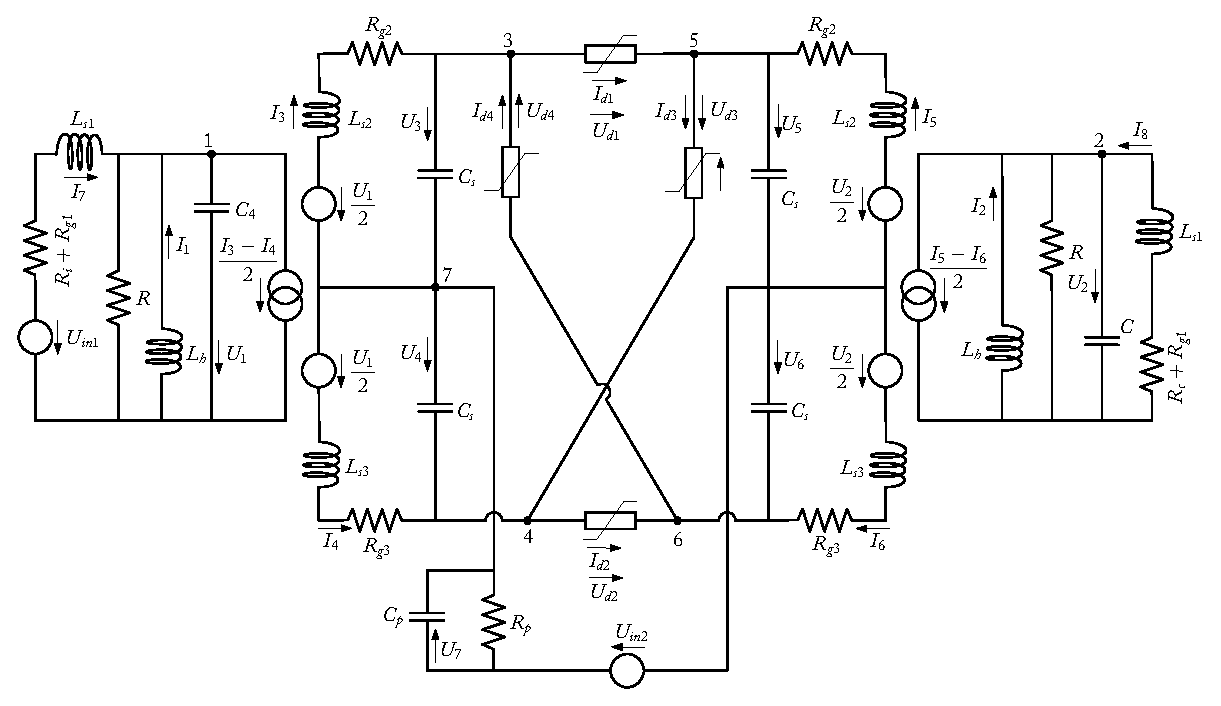
\includegraphics[width=1.0\textwidth]{figures/chapter_4/ring_modulator.eps}
  \caption{Electric ring modulator circuit~\cite{lioen1998test, mazzia2008test}.}
  \label{chap4:fig:ring_modulator}
\end{figure}

\begin{table}
  \caption{Expression complexity encountered throughout the index reduction of the electric ring modulator problem~\cite{lioen1998test, mazzia2008test} \ac{DAE} system index reduction. \emph{Legend}: $\cf$ = functions, $\ca$ = additions, $\cm$ = multiplications, and $\cd$ = divisions.}
  \label{chap4:tab:tppc_robot}
  \centering
  {\footnotesize\begin{tabular}{cccc}
    \multicolumn{4}{c}{\textbf{Electric Ring Modulator~\cite{lioen1998test, mazzia2008test}}} \\
    \toprule
    \textbf{Original \acp{DAE}} & \multicolumn{3}{c}{$\mF = 116\cf + 3\cd + 75\cm + 92\ca$ \quad $\mh = 0$} \\
    \midrule
    \textbf{Reduction step} & $\mE$ & $\mg$ & $\ma$ \\
    \midrule
    Index-2 \acp{DAE} & $0$ & $51\cf + 3\cd + 41\cm + 41\ca$ & $44\cf + 32\cm + 36\ca$ \\
    Index-1 \acp{DAE} & $86\cf + 68\cm + 66\ca$ & $262\cf + 13\cd + 416\cm + 220\ca$ & $10\cf + 2\cd + 18\cm + 11\ca$ \\
    Index-0 \acp{DAE} & $86\cf + 12\cd + 72\cm + 70\ca$ & $262\cf + 13\cd + 416\cm + 220\ca$ & $0$ \\
    \midrule
    \textbf{Reduced \acp{DAE}} & \multicolumn{3}{c}{$\mF = 335\cf + 15\cd + 537\cm + 256\ca$ \quad $\mh = 54\cf + 2\cd + 50\cm + 47\ca$} \\
    \bottomrule
    \end{tabular}}
\end{table}

\begin{figure}[htb]
  \centering
  \small{\includetikz{figures/chapter_4/ring_modulator.tex}}
  \caption{Electric ring modulator circuit integration results~\cite{lioen1998test, mazzia2008test} in the time interval $t \in \RSI{0}{1}{\milli\second}$. The lines represent the modulated output signal $U_2$, which is equal to the state variable $x_2$. \emph{Legend}: \textcolor{mycolor1}{$\blacksquare$} output signal $U_2$ with $C_s = \SSI{0}{\pico\farad}$ (\ac{DAE} system), \textcolor{mycolor2}{$\blacksquare$} output signal $U_2$ with $C_s = \SSI{2}{\pico\farad}$ (\ac{ODE} system).}
  \label{chap4:fig:ring_modulator_results}
\end{figure}

\subsection{Cascade of Differential Amplifiers}

The cascade of differential amplifiers is an example of a system whose index can be arbitrarily high, depending on how many operational amplifiers are cascaded. If we consider a circuit with one differential amplifier as shown in Figure~\ref{chap:4:fig:diffamp_single} and, assuming that the operational amplifier is ideal, the circuit equations lead to the relation $x(t) = -C R U(t)^{\prime}$ where $U(t)$ is the generator voltage. Since the solution to the circuit equations involves at least one derivative of the input function, the system must be index-1. By cascading a series of $p \in \mathcal{N}$ differential amplifiers in a circuit as in Figure~\ref{chap:4:fig:diffamp_cascade}, we can see that the resulting \acp{DAE} index is equal to $p$. Specifically, the voltage at the output of the $p$-th differential amplifier is given by $x_p(t) = -C_p R_p x_{p-1}(t)^{\prime}$, where $v(t) = -C_1 R_1 U(t)^{\prime}$. Thence the following system of equations is obtained
%
\begin{equation*}
  \begin{cases}
    x_1(t) = -C_1 R_1 U(t)^{\prime} \\
    x_2(t) = -C_2 R_2 x_1(t)^{\prime} \\
    ~\vdots \\
    x_p(t) = -C_p R_p x_{p-1}(t)^{\prime}
  \end{cases}
  %
  \quad \text{whose analytical solution is} \quad
  %
  x_i(t) = \prod_{j=1}^{i} (-C_j R_j) \dfrac{\de{}^{i}}{\de{}t^{i}}U(t) \, \text{.}
\end{equation*}
%
Consistent initial conditions at $t = t_0$ can be easily obtained by evaluating the analytical solution at $t = t_0$, \ie{},
%
\begin{equation*}
  \m{x}_0 = \begin{bmatrix}
    -C_1 R_1 \left.\dfrac{\de{}}{\de{}t}U(t)\right|_{t=t_0} \\
    \vdots \\
    \displaystyle\prod_{j=1}^{p} (-C_j R_j) \left.\dfrac{\de{}^{p}}{\de{}t^{p}}U(t)\right|_{t=t_0}
  \end{bmatrix} \, \text{.}
\end{equation*}

\begin{figure}[htb]
  \centering
  \begin{subfigure}[t]{0.26\textwidth}
    \centering
    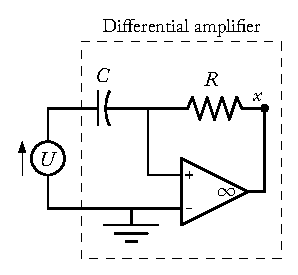
\includegraphics[width=1.0\textwidth]{figures/chapter_4/differential_amplifier_single.eps}
    \caption{Circuit with a single differential amplifier.}
    \label{chap:4:fig:diffamp_single}
  \end{subfigure}%
  \hfill%
  \begin{subfigure}[t]{0.72\textwidth}
    \centering
    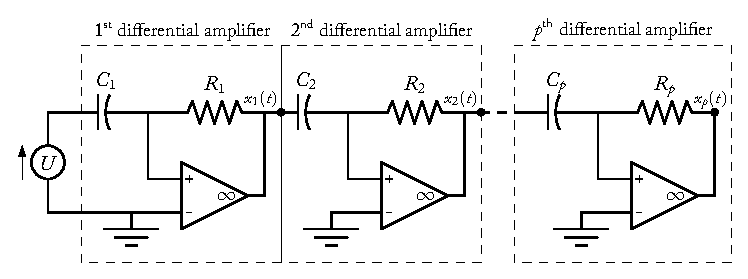
\includegraphics[width=1.0\textwidth]{figures/chapter_4/differential_amplifier_cascade.eps}
    \caption{Circuit with a cascade of $p$ differential amplifiers.}
    \label{chap:4:fig:diffamp_cascade}
  \end{subfigure}
  \caption{Circuit diagrams for the cascade of differential amplifiers problem~\cite{brenan1995numerical}.}
  \label{chap:4:fig:diffamp_all}
\end{figure}

The index reduction of such a system, which falls under the category of linear \acp{DAE}, is pretty much straightforward. \Indigo{} can reduce to index-0 systems made of up to $p = 100$ differential amplifiers, even if the performance of the reduction process is strongly linked to the capabilities of \Maple{} symbolic kernel to deal with sparse large matrices. An interesting aspect that this last application brings to light is how systematically the index reduction process is performed through \Indigo{}. The system is transformed in the form $\mE \, \mx = \mg$ with $\ma = \m{0}$, which is explicitly given by
%
\begin{equation*}
  \left[\begin{array}{ccc|c}
    -C_2 R_2 & & & 0 \\
    & \ddots & & \vdots \\
    & & -C_p R_p & 0 \\
  \end{array}\right]
  %
  \left[\begin{array}{c}
    x_1^{\prime} \\ \vdots \\ x_{p-1}^{\prime} \\ \hline x_p^{\prime}
  \end{array}\right] = \left[\begin{array}{c}
    x_2 \\ \vdots \\ x_p
  \end{array}\right]
  %
  \quad \text{with} \quad
  %
  \ma = \begin{bmatrix}
    - x_1 - C_1 R_1 \dfrac{\de{}}{\de{}t}U(t)
  \end{bmatrix} \, \text{.}
\end{equation*}
%
Then the index reduction is performed $p$ times, and the system $\mE \, \mx = \mg$ at the $k$-th index reduction step is given by
%
\begin{equation*}
  \left[\begin{array}{ccc|c|ccc}
    1 &        &   & \\
      & \ddots &   & \\
      &        & 1 & \\ \hline
      &        &   & & -C_{k+2} R_{k+2} \\
      &        &   & & & \ddots \\
      &        &   & & & & -C_{p} R_{p} \\ \hline
      &        &   & 1 \\
  \end{array}\right]
  %
  \left[\begin{array}{c}
    x_1^{\prime} \\ \vdots \\ x_{k+1}^{\prime} \\ \hline
    x_{k+2}^{\prime} \\ \vdots \\ x_{p-1}^{\prime} \\ \hline
    x_p^{\prime}
  \end{array}\right] = \left[\begin{array}{c}
    -C_1R_1 \dfrac{\de{}^2}{\de{}t^2}U(t) \\
    \vdots \\
    \displaystyle\prod_{j=1}^{k-1} (-C_j R_j) \dfrac{\de{}^k}{\de{}t^k}U(t) \\ \hline
    x_{k+2} \\ \vdots \\ x_p \\ \hline
    \displaystyle\prod_{j=1}^{k} (-C_j R_j) \dfrac{\de{}^{k+1}}{\de{}t^{k+1}}U(t)
  \end{array}\right] \, \text{,}
\end{equation*}
%
with algebraic equations $\ma = \m{0}$ and hidden constraints $\mh = \m{0}$ given by
%
\begin{equation*}
  \ma = \begin{bmatrix}
    -x_{k+1} + \displaystyle\prod_{j=1}^{k+1} (-C_j R_j) \dfrac{\de{}^{k+1}}{\de{}t^{k+1}}U(t)
  \end{bmatrix}
  %
  \quad \text{and} \quad
  %
  \mh = \begin{bmatrix}
    -x_{1} - C_1R_1 \dfrac{\de{}}{\de{}t}U(t) \\
    \vdots \\
    -x_k + \displaystyle\prod_{j=1}^{k} (-C_j R_j) \dfrac{\de{}^{k}}{\de{}t^{k}}U(t)
  \end{bmatrix} \, \text{.}
\end{equation*}
%
The reduced index-0 system is then given by
%
\begin{equation*}
  \begin{bmatrix}
    1 & & \\
    & \ddots & \\
    & & 1 \\
  \end{bmatrix}
  %
  \begin{bmatrix}
    x_1^{\prime} \\ \vdots \\ x_p^{\prime}
  \end{bmatrix} = \left[\begin{array}{c}
    -C_1R_1 \dfrac{\de{}^{2}}{\de{}t^{2}}U(t) \\
    \vdots \\
    \displaystyle\prod_{j=1}^{p-1} (-C_j R_j) \dfrac{\de{}^{p}}{\de{}t^{p}}U(t)
  \end{array}\right]
  %
  \quad \text{with} \quad
  %
  \mh = \begin{bmatrix}
    -x_{1} - C_1R_1 \dfrac{\de{}}{\de{}t}U(t) \\
    \vdots \\
    -x_k + \displaystyle\prod_{j=1}^{p} (-C_j R_j) \dfrac{\de{}^{p}}{\de{}t^{p}}U(t)
  \end{bmatrix} \, \text{.}
\end{equation*}
%

% % % % % % % % % % % % % % % % % % % % % % % % % % % % % % % % % % % % % % % %

\section{Summary of Results and Discussion}

It is now time to summarize the results obtained from the experiments and discuss the performance of the presented algorithm. To do so we will consider the following aspects: the symbolic index reduction, the numerical integration, and the overall performance of the algorithm. The results are summarized in Table~\ref{chap4:tab:numerical_integration}, where for each example the solution process is summarized in brief. It is important to highlight that in the same table, the examples are numbered according to the order in which they were presented in this chapter, which will be useful for the discussion that follows.

\subsection{Symbolic Index Reduction}

The first aspect to consider is the symbolic index reduction process. Specifically, the presented algorithm can successfully reduce the index of all the example \ac{DAE} systems here considered. The computational cost of the expressions generated during the index reduction procedure is comparable to the original \ac{DAE} system in most of the tests. However, in examples 3, 6, 7 and 11 the expressions generated during the index reduction procedure are significantly more complex than the original \ac{DAE} system. In these cases, the \Maple{} symbolic computation kernel is not able to perform the simplification within \SI{100}{\second} of CPU time and the raw expressions are kept in the following reduction steps. As a consequence, the computational cost inherently increases throughout the following reduction steps. Notably, the \ac{DAE} systems that are hard to simplify are those having a matrix $\mA$ that is strongly dependent on the state variables $\mx$ or equivalently that retains complicated divisions in the vector $\mb$. In these cases, the computational cost of the vector $\ma$ increases significantly due to successive and repeated differentiation and symbolic factorization. In examples 3, 6, 7 and 11, the hierarchical pivoting strategy is then used to mitigate the expression swell and ensure the successful index reduction of the \ac{DAE} system. In examples 3 and 11 the veiling strategy proved to be of substantial help, effectively reducing the expression complexities and ensuring the successful index reduction of the \ac{DAE} system. In examples 6 and 7, the hierarchical representation is not used on purpose to understand the impact of the expression swell on the numerical integration process.

It worth mentioning that the trigonometric identities provided by Weierstra{\ss}~\eqref{chap2:eq:weierstrass} or~\eqref{chap2:eq:zhou} can be used to obtain polynomial expressions and improve the detection of symbolic eliminations (see Section~\ref{chap2:sec:signature}). However, the use of such trigonometric identities does not typically lead to a significant improvement in the computational cost of the expressions generated during the index reduction procedure as the polynomial expressions obtained are hard to simplify as well. Furthermore, such transformations impose a change of coordinates in the original \ac{DAE} system, which may be undesirable in some applications.

Another aspect that is important to mention is the sudden increase in computational complexity of the expressions generated in the last reduction step. Even if this increase is not critical to the correct index reduction as the presented algorithm is robust to expression swell, it does undermine the numerical efficiency of the final \ac{DAE} system. This highlights the need for further research on expression swell mitigation techniques in symbolic computation (see Section~\ref{chap2:sec:lem}), as well as the need to use integrators that can handle index-1 or even index-2 \acp{DAE}.

\subsection{Numerical Integration}

The numerical integration for the remaining examples is also carried out, with outcomes detailed in Table~\ref{chap4:tab:numerical_integration}. This table reports the performance comparison between the joint index reduction algorithm and numerical integration schemes offered by \Maple{} and those of \Indigo{}. To ensure a fair comparison, both \Maple{} and \Indigo{} utilize the Runge-Kutta-Fehlberg 4(5) method for numerical integration of the \ac{DAE} system. Identical error tolerances are applied, with a relative tolerance of $10^{-6}$ and an absolute tolerance of $10^{-7}$. The results illustrate that the \Indigo{}'s index reduction algorithm implementation effectively generates numerically stable reduced-index \acp{DAE}, ensuring consistent integration across examples. However, exceptions arise in examples 3, 5, 6, 7, 9, 10, 11, 13, and 14. Specifically, in examples 3, 5, 6, 7, 9, 11, and 13, \Maple{} fails to generate code for the reduced-index system within the expected time frame, thus the integration is not performed. This is due to the complexity of the expressions generated during the index reduction procedure, which overloads the \Maple{}'s \texttt{CodeGeneration} package. On the other hand in examples 10 and 14, the numerical integration can not be performed due to the inability of \Maple{} to verify the consistency of the \ac{IVP}. The \Indigo{} numerical integration is successful in all examples, except for example 11, where it fails to generate the code for the reduced-index system within the expected time frame. This is due to the complexity of the expressions generated during the index reduction procedure, which overloads the \Indigo{}'s \texttt{CodeGeneration} package. Notably, in examples 5, 6 and 7 the integration of the reduced-index system is successfully performed using the non-default implicit RadauIIA5 method. Nonetheless, the high expression swell in these examples lead to a significant increase in the computational cost of the numerical integration, however, the numerical stability is not compromised. Notice that \Maple{}'s \texttt{dsolve} exceeded the function evaluations limit during the numerical integration of these examples due to either system's stiffness or high index.

It is important to highlight that during the numerical integration, the symbolic code is not regenerated by updating the index reduction. Therefore, for some numerical values of states and parameters, the \acp{DAE} system structure may change, leading to numerical instability. While this does pose a potential issue, it is worth noting that we have not encountered instability in the integration process, proving that the presented pivoting strategy is effective.

\setlength\tabcolsep{2.5pt}
\setlength{\LTcapwidth}{\textwidth}
{\footnotesize\centering\begin{longtable}{lccl}
  \caption{Numerical integration results of the reduced-index \ac{DAE} systems. The table reports the name and reference of the \ac{DAE} system, the index of the system, the integration interval $t \in [t_{\text{ini}}, \, t_{\text{end}}]$, and the outcomes of the whole code generation and integration process for both \Maple{} and \Indigo{}. If not otherwise specified, the tests are integrated using a Runge-Kutta-Fehlberg 4(5) method with a relative tolerance of $10^{-6}$ and an absolute tolerance of $10^{-7}$. The computation time limit is \SI{1000}{\second}, to both generate the necessary code and perform numerical computations. \emph{Legend:} \mycheckmark{} successful code generation and numerical integration, \mycrossmark{} errors in the code generation, numerical integration or time expired, and \mywarnmark{} warnings encountered or non-default settings used in the code generation or numerical integration.}
  \label{chap3:tab:numerical_integration}
  \endfirsthead
  \endhead
  %
  \toprule
  \textbf{Integrated \ac{DAE} system} &
  \multicolumn{3}{l}{\textbf{Integration outcomes and errors}} \\
  \midrule
  \multirow{1}{*}{\textbf{1.~~Particle Motion~\cite{campbell1995constraint}}}
    & \Maple{}  & \mycheckmark{}\phantom{\mywarnmark{}} & Success \\ \cmidrule(l{4pt}){2-4}
    Index-3 \quad $t \in [0, 400\pi]$ seconds & \Indigo{} & \mycheckmark{}\phantom{\mywarnmark{}} & Success \\ \midrule
  \multirow{1}{*}{\textbf{2.~~Car-Axis~\cite{lioen1998test, mazzia2008test}}}
    & \Maple{}  & \mycheckmark{}\phantom{\mywarnmark{}} & Success \\ \cmidrule(l{4pt}){2-4}
    Index-3 \quad $t \in [0, 3]$ seconds & \Indigo{} & \mycheckmark{}\phantom{\mywarnmark{}} & Success \\ \midrule
  \multirow{1}{*}{\textbf{3.~~Flexible Slider-Crank~\cite{lioen1998test, mazzia2008test}}}
    & \Maple{}  & \mycrossmark{}\phantom{\mywarnmark{}} & Error, time expired (in \texttt{dsolve}) \\ \cmidrule(l{4pt}){2-4}
    Index-3 \quad $t \in [0, 0.1]$ seconds & \Indigo{} & \mycheckmark{}\phantom{\mywarnmark{}} & Success \\ \midrule
  \multirow{1}{*}{\textbf{4.~~2-Pendula~\cite{pryce1998solving}}}
    & \Maple{}  & \mycheckmark{}\phantom{\mywarnmark{}} & Success \\ \cmidrule(l{4pt}){2-4}
    Index-5 \quad $t \in [0, 60]$ seconds & \Indigo{} & \mycheckmark{}\phantom{\mywarnmark{}} & Success \\ \midrule
  \multirow{1}{*}{\textbf{5.~~3-Pendula~\cite{nedialkov2008solvingIII}}}
    & \Maple{}  & \mycrossmark{}\phantom{\mywarnmark{}} & Error, time expired (in \texttt{dsolve}) \\ \cmidrule(l{4pt}){2-4}
    Index-7 \quad $t \in [0, 60]$ seconds & \Indigo{} & \mycheckmark{}\mywarnmark{} & Success with RadauIIA5 method \\ \midrule
  \multirow{1}{*}{\textbf{6.~~4-Pendula~\cite{nedialkov2008solvingIII}}}
      & \Maple{}  & \mycrossmark{}\phantom{\mywarnmark{}} & Error, time expired (in \texttt{dsolve}) \\ \cmidrule(l{4pt}){2-4}
      Index-9 \quad $t \in [0, 60]$ seconds & \Indigo{} & \mycheckmark{}\mywarnmark{} & Success with RadauIIA5 method \\ \midrule
  \multirow{1}{*}{\textbf{7.~~5-Pendula~\cite{nedialkov2008solvingIII}}}
      & \Maple{}  & \mycrossmark{}\phantom{\mywarnmark{}} & Error, time expired (in \texttt{dsolve}) \\ \cmidrule(l{4pt}){2-4}
      Index-11 \quad $t \in [0, 60]$ seconds & \Indigo{} & \mycheckmark{}\mywarnmark{} & Success with RadauIIA5 method \\ \midrule
  \multirow{1}{*}{\textbf{8.~~Double-Wishbone Suspension}}
    & \Maple{}  & \mycheckmark{}\phantom{\mywarnmark{}} & Success \\ \cmidrule(l{4pt}){2-4}
    Index-3 \quad $t \in [0, 60]$ seconds & \Indigo{} & \mycheckmark{}\phantom{\mywarnmark{}} & Success \\ \midrule
  \multirow{1}{*}{\textbf{9.~~Initial Stage Space Shuttle Reentry~\cite{brenan1995numerical}}}
    & \Maple{}  & \mycrossmark{}\phantom{\mywarnmark{}} & Error, time expired (in \texttt{dsolve}) \\ \cmidrule(l{4pt}){2-4}
    Index-3 \quad $t \in [332.8, 419.8]$ seconds & \Indigo{} & \mycheckmark{}\phantom{\mywarnmark{}} & Success \\ \midrule
  \multirow{1}{*}{\textbf{10.~~Final Stage Space Shuttle Reentry~\cite{brenan1995numerical}}}
    & \Maple{}  & \mycrossmark{}\phantom{\mywarnmark{}} & Error, in \texttt{dsolve/numeric/DAE/checkconstraints} \\ \cmidrule(l{4pt}){2-4}
    Index-2 \quad $t \in [0, 300]$ seconds & \Indigo{} & \mycheckmark{}\phantom{\mywarnmark{}} & Success \\ \midrule
  \multirow{1}{*}{\textbf{11.~~Robotic Arm~\cite{pryce1998solving}}}
    & \Maple{}  & \mycrossmark{}\phantom{\mywarnmark{}} & Error, time expired (in \texttt{dsolve}) \\ \cmidrule(l{4pt}){2-4}
    Index-5 \quad $t \in [0, 2]$ seconds & \Indigo{} & \mycrossmark{}\phantom{\mywarnmark{}} & Error, time expired (in \texttt{CodeGeneration}) \\ \midrule
  \multirow{1}{*}{\textbf{12.~~Eight-Nodes Transistor-Amplifier~\cite{lioen1998test, mazzia2008test}}}
    & \Maple{}  & \mycheckmark{}\mywarnmark{} & Warning, function evaluations limit exceeded \\ \cmidrule(l{4pt}){2-4}
    Index-1 \quad $t \in [0, 0.2]$ seconds & \Indigo{} & \mycheckmark{}\phantom{\mywarnmark{}} & Success \\ \midrule
  \multirow{1}{*}{\textbf{13.~~Electric Ring Modulator~\cite{lioen1998test, mazzia2008test}}}
    & \Maple{}  & \mycrossmark{}\phantom{\mywarnmark{}} & Error, time expired (in \texttt{dsolve}) \\ \cmidrule(l{4pt}){2-4}
    Index-2 \quad $t \in [0, 1]$ milliseconds & \Indigo{} & \mycheckmark{}\phantom{\mywarnmark{}} & Success \\ \midrule
  \multirow{1}{*}{\textbf{14.~~Cascaded Differential Amplifiers~\cite{brenan1995numerical}}}
    & \Maple{}  & \mycrossmark{}\phantom{\mywarnmark{}} & Error, in \texttt{dsolve/numeric/DAE/checkconstraints} \\ \cmidrule(l{4pt}){2-4}
    Arbitrary high index \quad $t \in [0, 10]$ seconds & \Indigo{} & \mycheckmark{}\phantom{\mywarnmark{}} & Success \\
  \bottomrule
  %
\end{longtable}}

